\graphicspath{{chapt_dutch/}{intro/}{chapt2/}{chapt3/}{chapt4/}{chapt5/}{chapt6/}{chapt7/}}

% Header
\renewcommand\evenpagerightmark{{\scshape\small Appendix B}}
\renewcommand\oddpageleftmark{{\scshape\small Validation of the generation procedure for interferenc}}

\renewcommand{\bibname}{References}

\hyphenation{}

\chapter[Validation of the generation procedure for interference]%
{Validation of the generation procedure for interference}\label{app3}
%
The generation procedure for the interference contribution, described in \ref{sec:sig_gen_val}, is validated for the case of a pseudoscalar of mass 500~GeV and partial width 10\%.
Both top quarks in the final state are required to decay semileptonically.
For this study, the factorization and renormalization scales are fixed to half of the mass of the particle, i.e 250~GeV.
Three different samples are generated:
\begin{itemize}
\item full $gg \rightarrow t\bar t$ production, including SM and BSM processes (40~M events, referred to as ``ALL'' in the plots),
\item the SM contribution only (40~M events, referred to as ``SM'' in the plots),
\item the resonant BSM process (400~k events, referred to as ``R'' in the plots).
\end{itemize}
A set of kinematic variables are scrutinized with the aim to validate the generation procedure.
For each variable, histograms are filled from the three samples, taking the respective leading-order cross sections into account.
Histograms for the latter two samples are then subtracted from the distribution for the full process, resulting in the histogram denoted as ALL-SM-R in the plots legend.
In Figs~\ref{fig:comparison_top} to \ref{fig:comparison_tophel} the resulting distributions for the interference (in blue) are compared to the ones obtained as described in \ref{sec:sig_gen_val} (in red, denoted as I in the plots legend).
The plots show variables at the generator level, before any reconstruction simulation.
Apart from some fluctuations, no evident and significant discrepancy is observed and the method is considered validated.

\begin{figure} \centering
  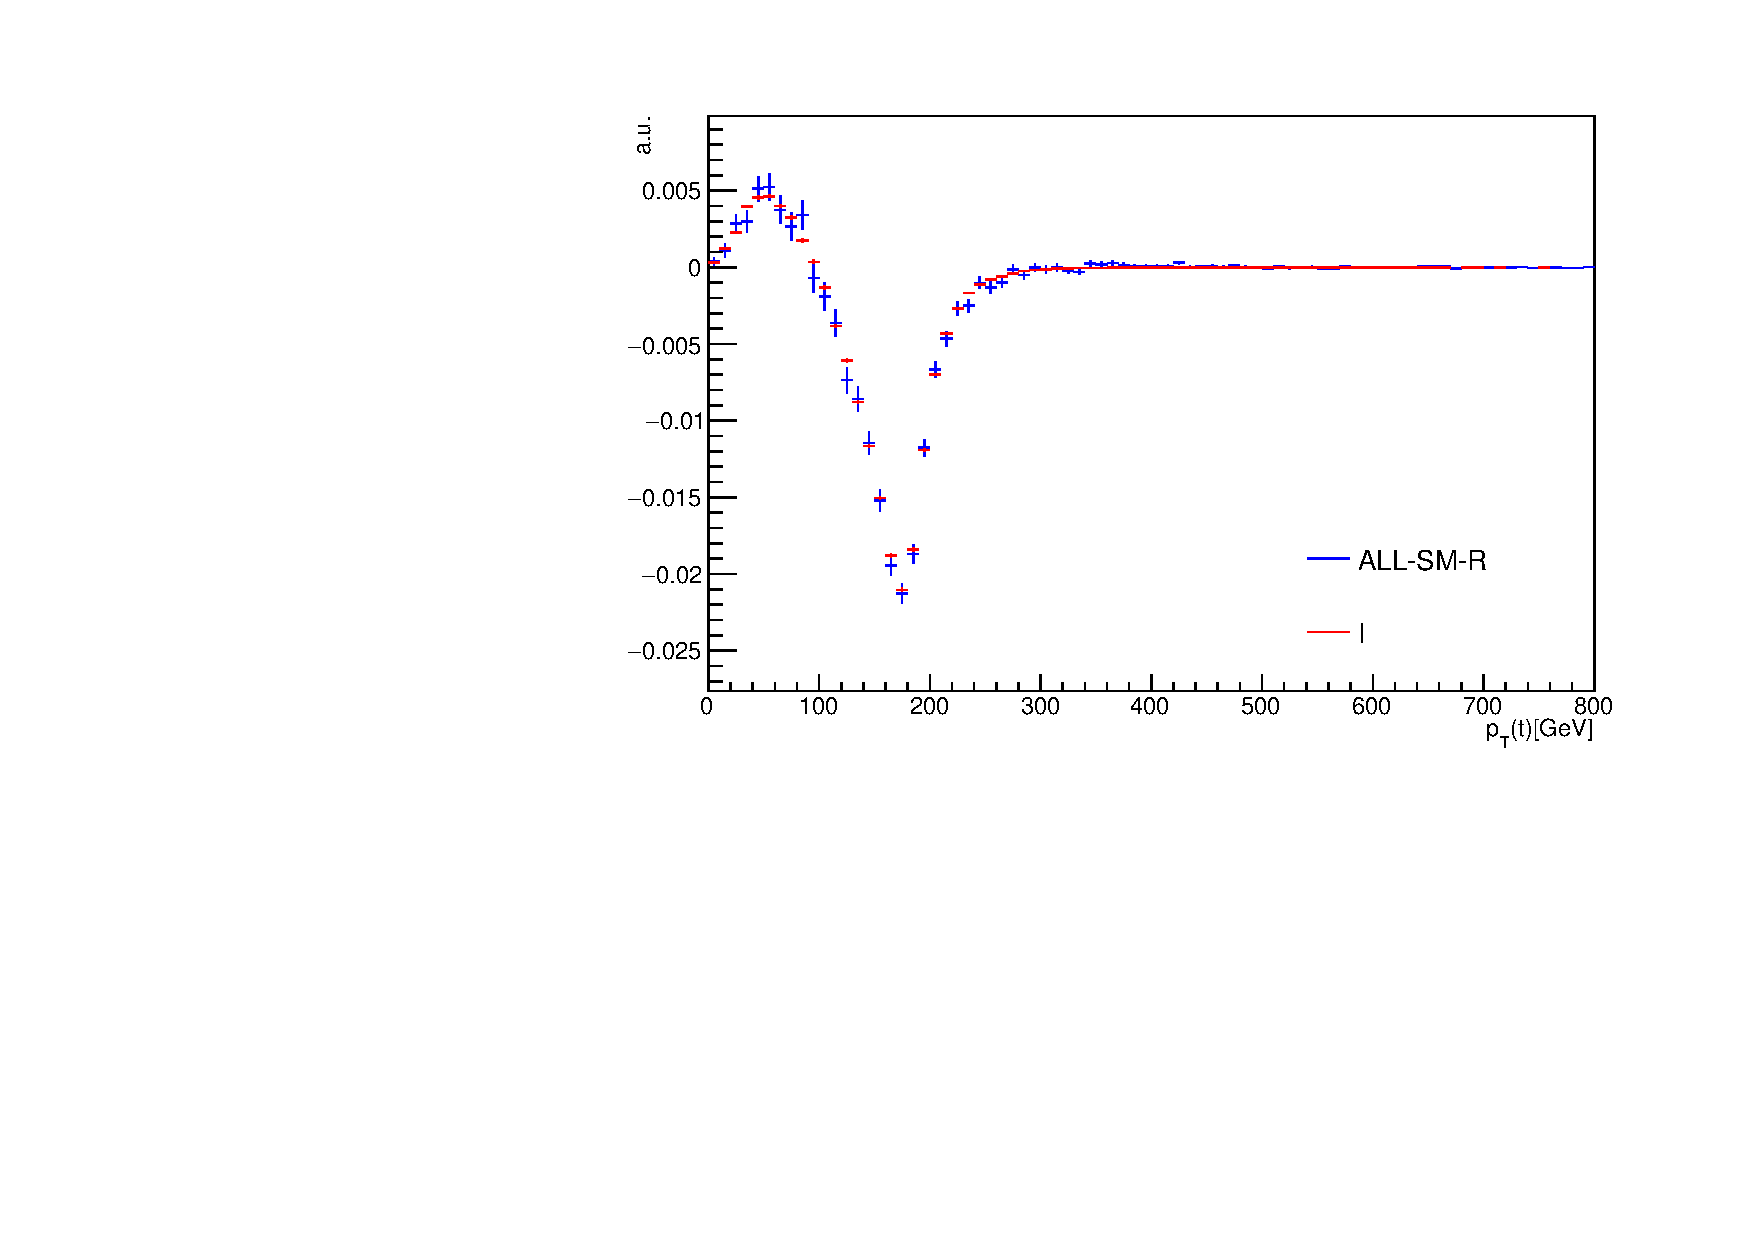
\includegraphics[width=0.4\textwidth]{fig/chapt4/gen_plots/top_pt_compare.pdf}
  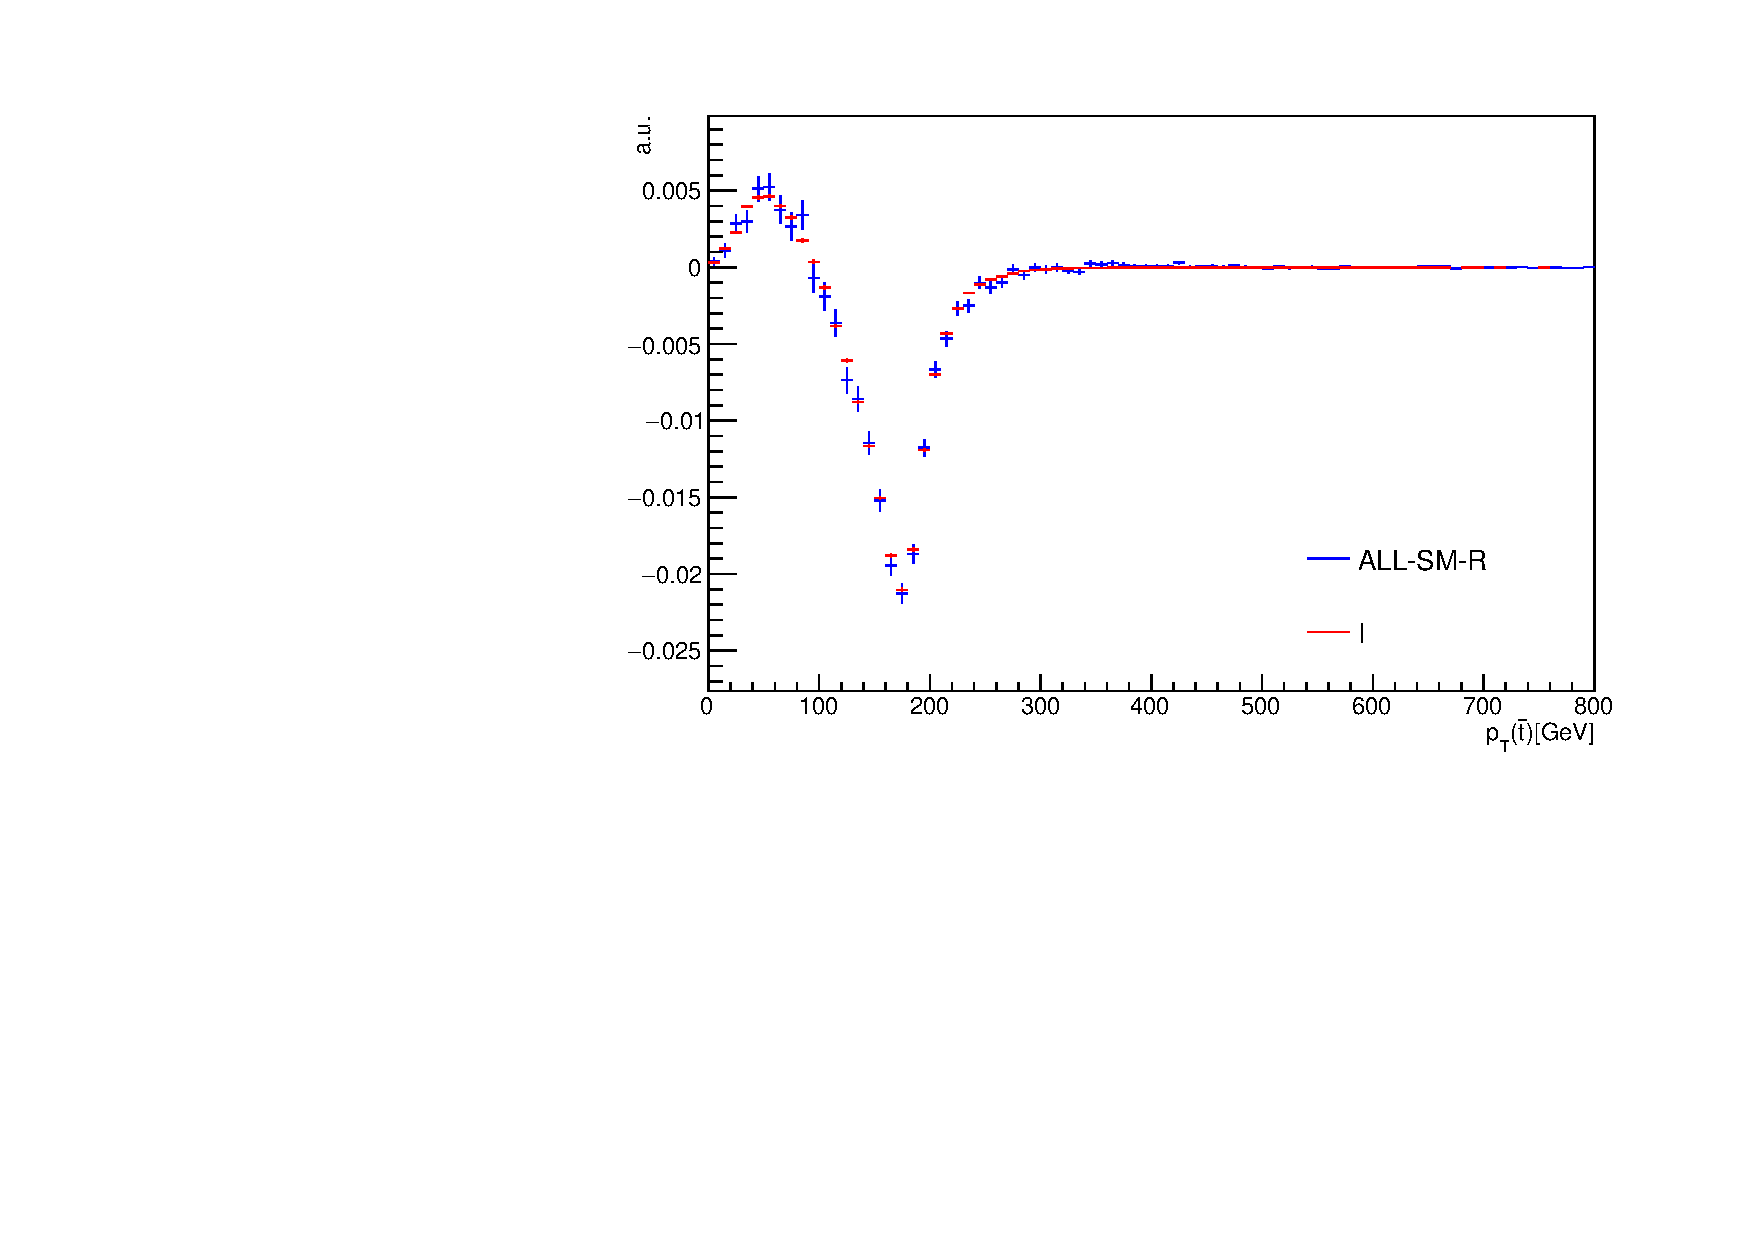
\includegraphics[width=0.4\textwidth]{fig/chapt4/gen_plots/tbar_pt_compare.pdf}\\
  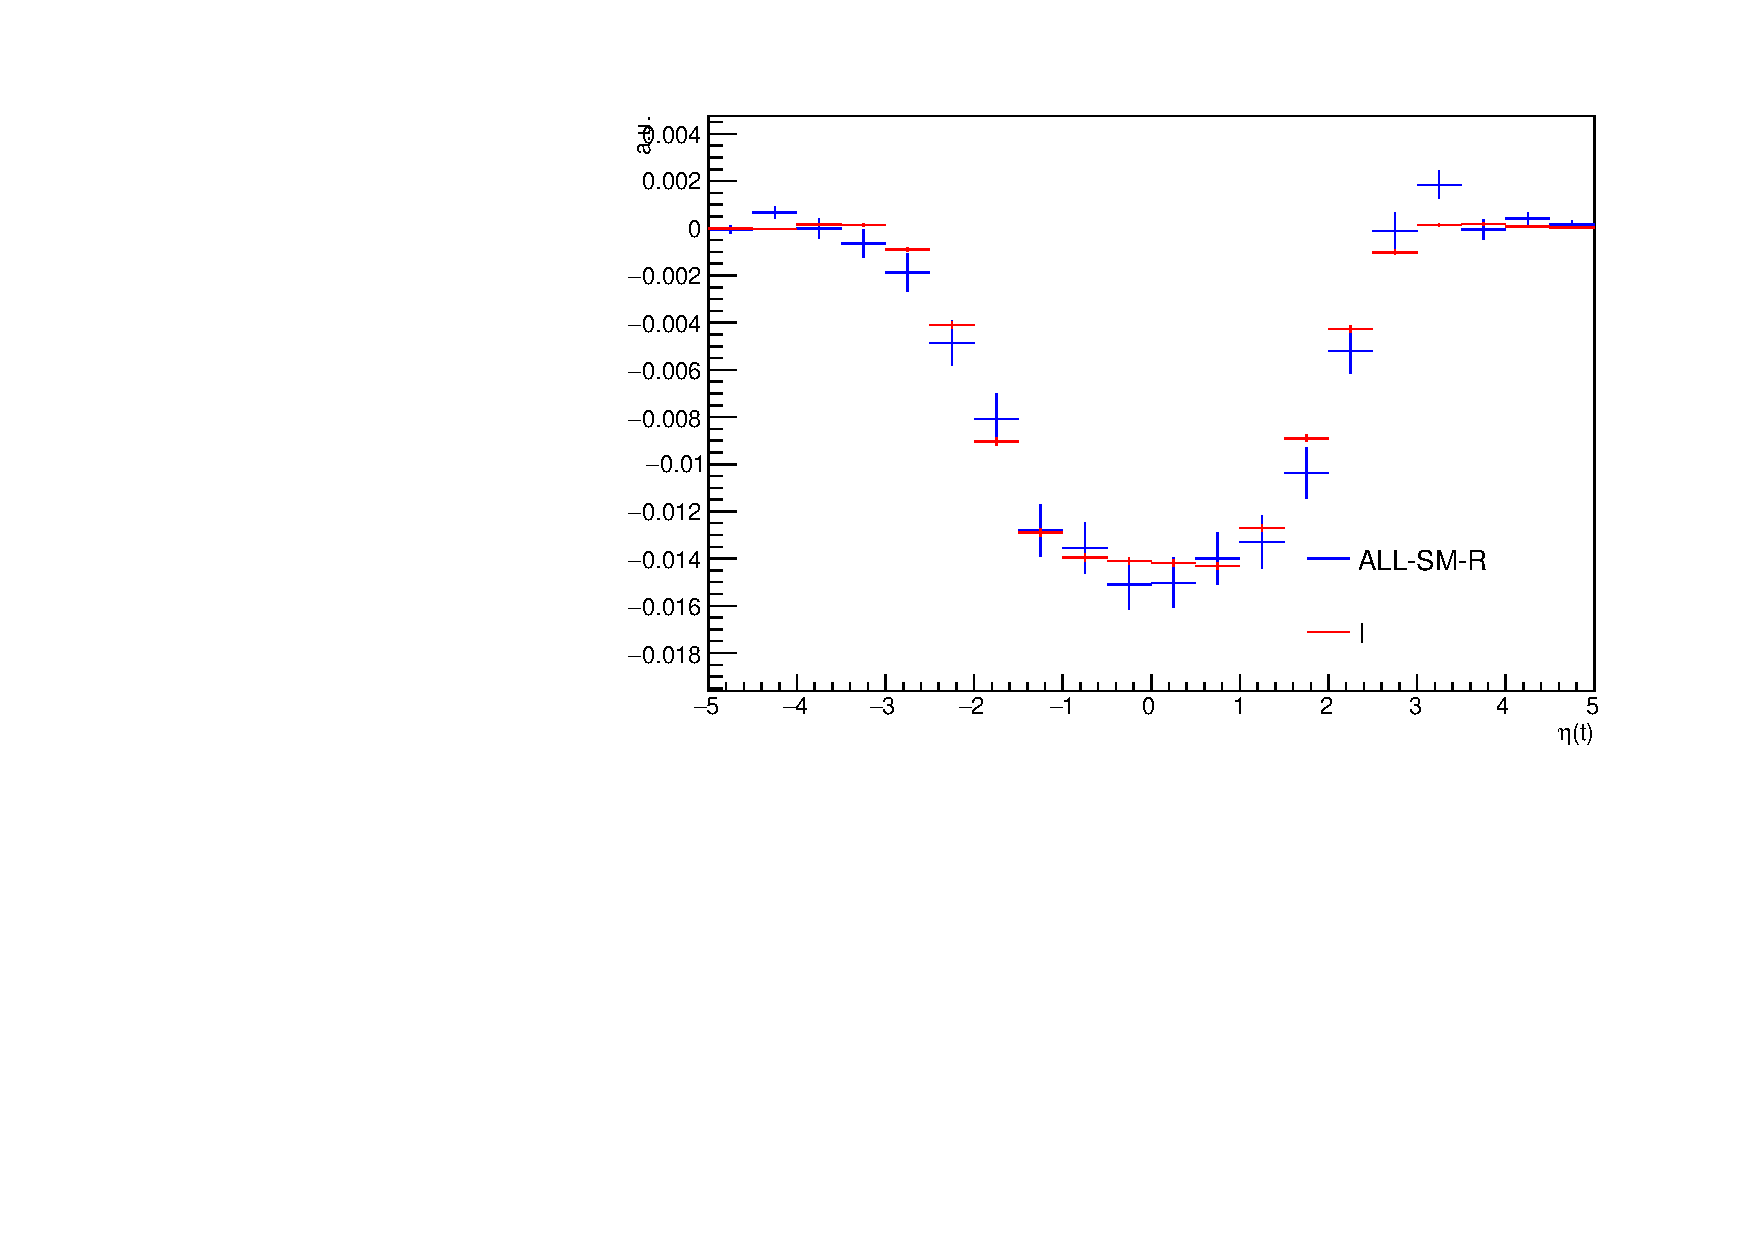
\includegraphics[width=0.4\textwidth]{fig/chapt4/gen_plots/top_eta_compare.pdf}
  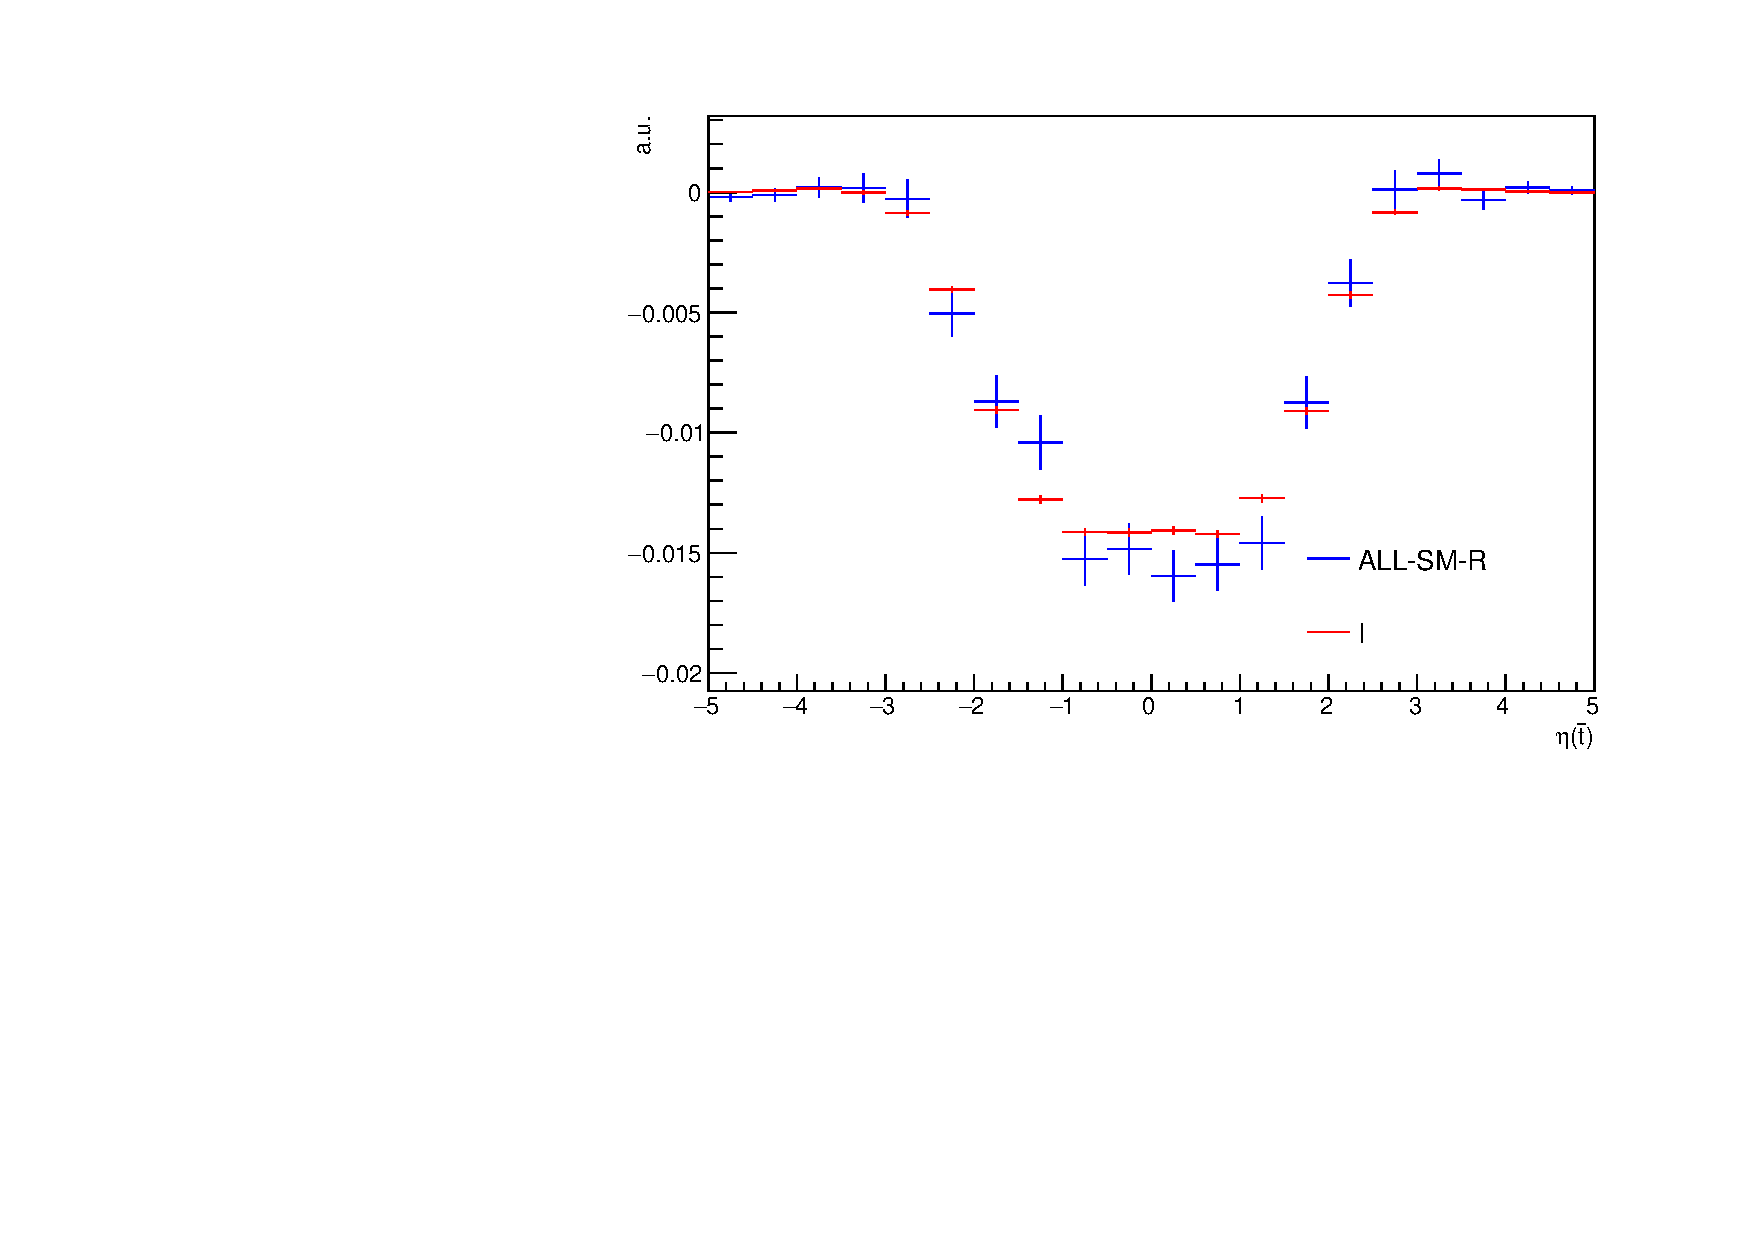
\includegraphics[width=0.4\textwidth]{fig/chapt4/gen_plots/tbar_eta_compare.pdf}\\
  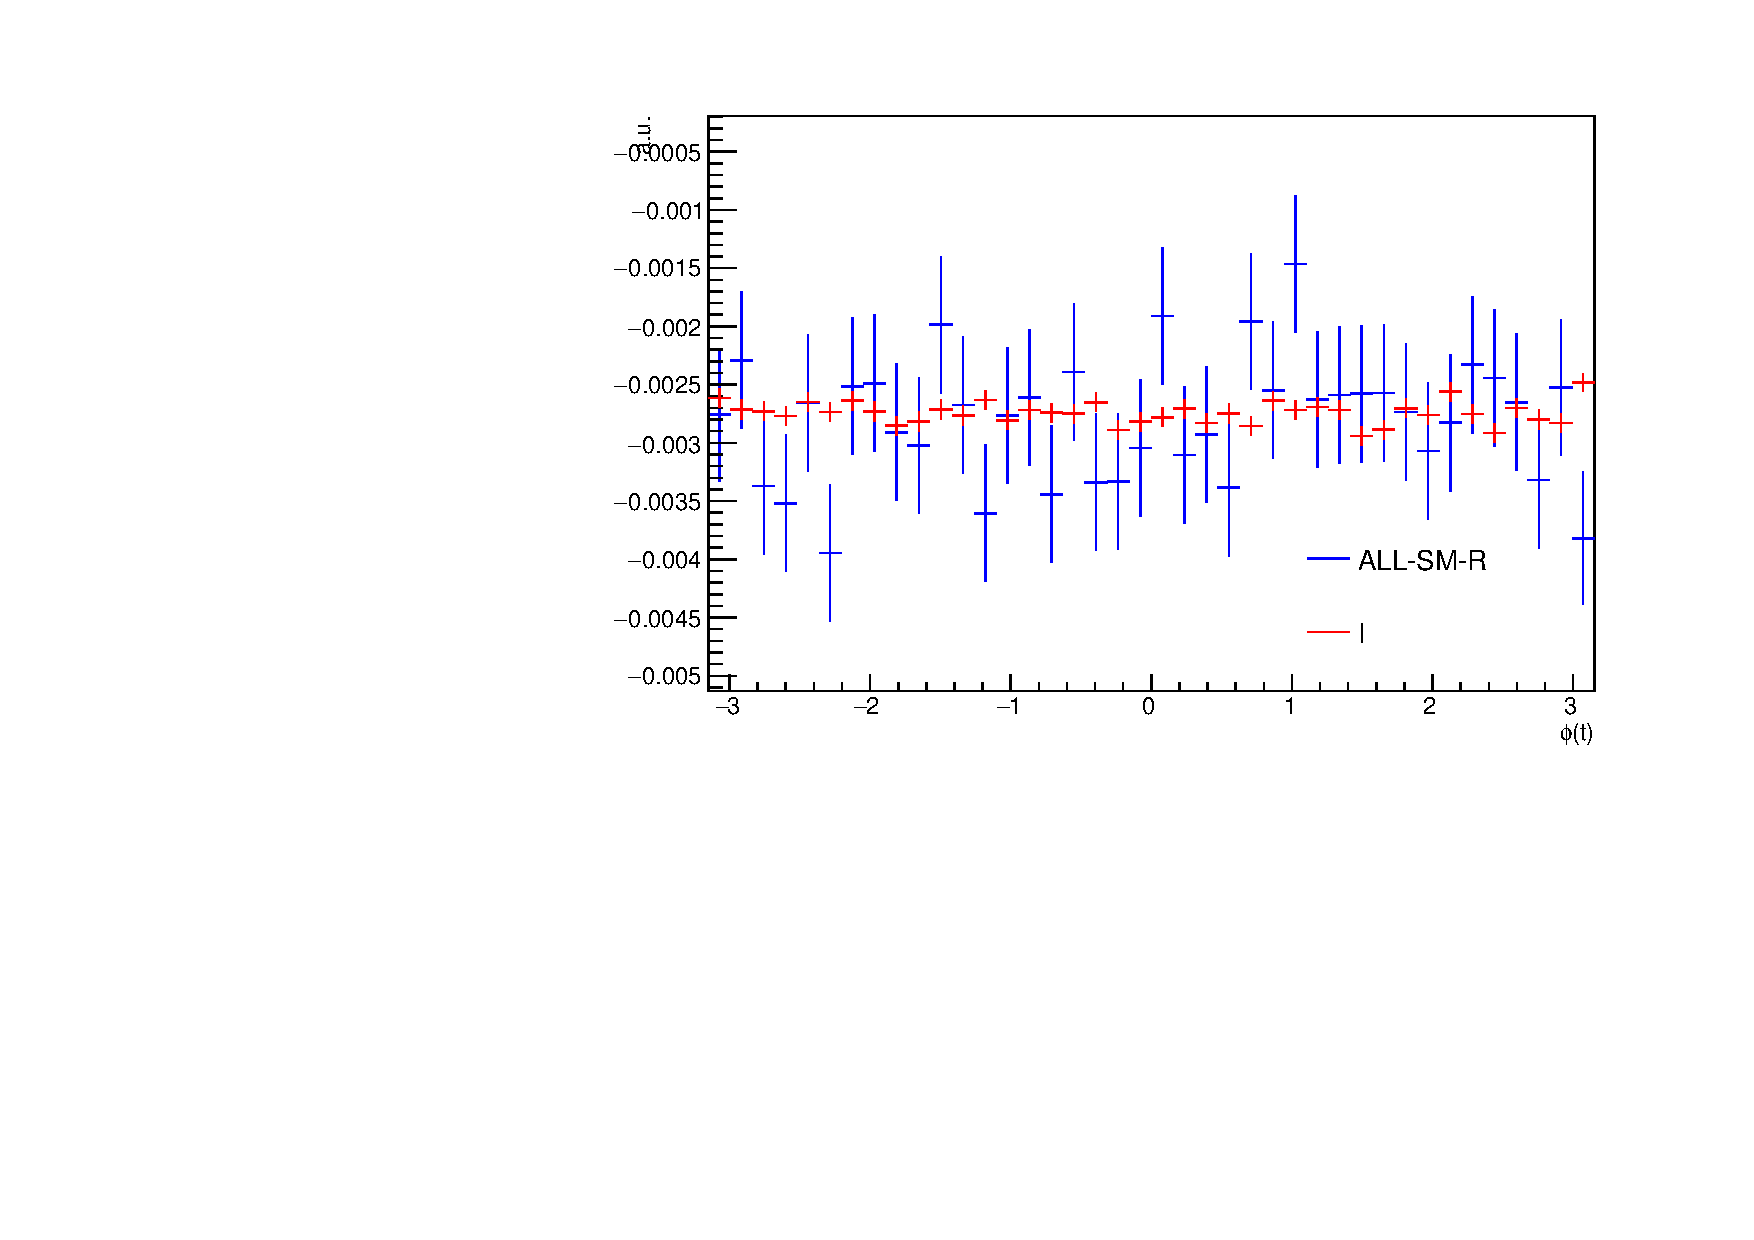
\includegraphics[width=0.4\textwidth]{fig/chapt4/gen_plots/top_phi_compare.pdf}
  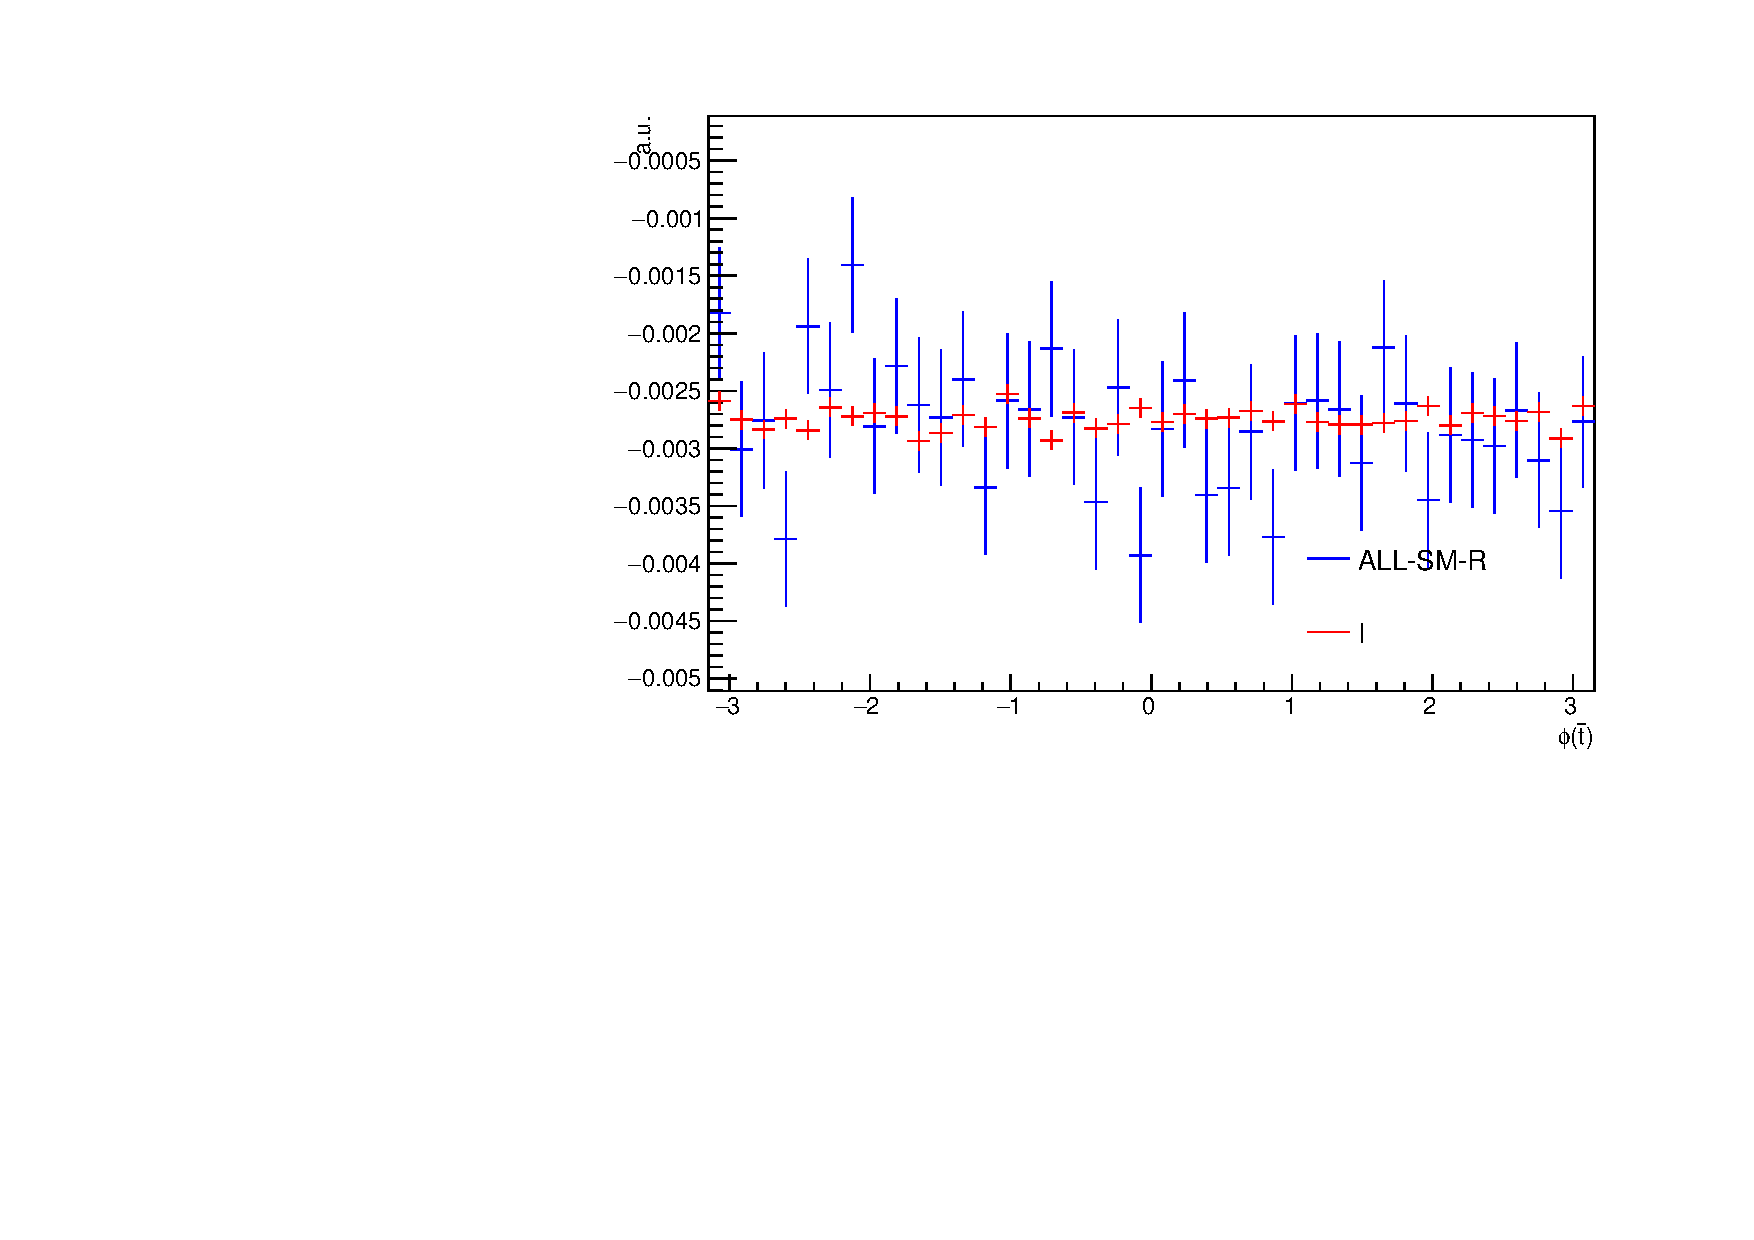
\includegraphics[width=0.4\textwidth]{fig/chapt4/gen_plots/tbar_phi_compare.pdf}
  \caption{Distributions of the transverse momenta, pseudorapidities, and azimuthal angles for top quark and antiquark. Comparison of the two approaches to model the interference.}
  \label{fig:comparison_top}
\end{figure}

\begin{figure} \centering
  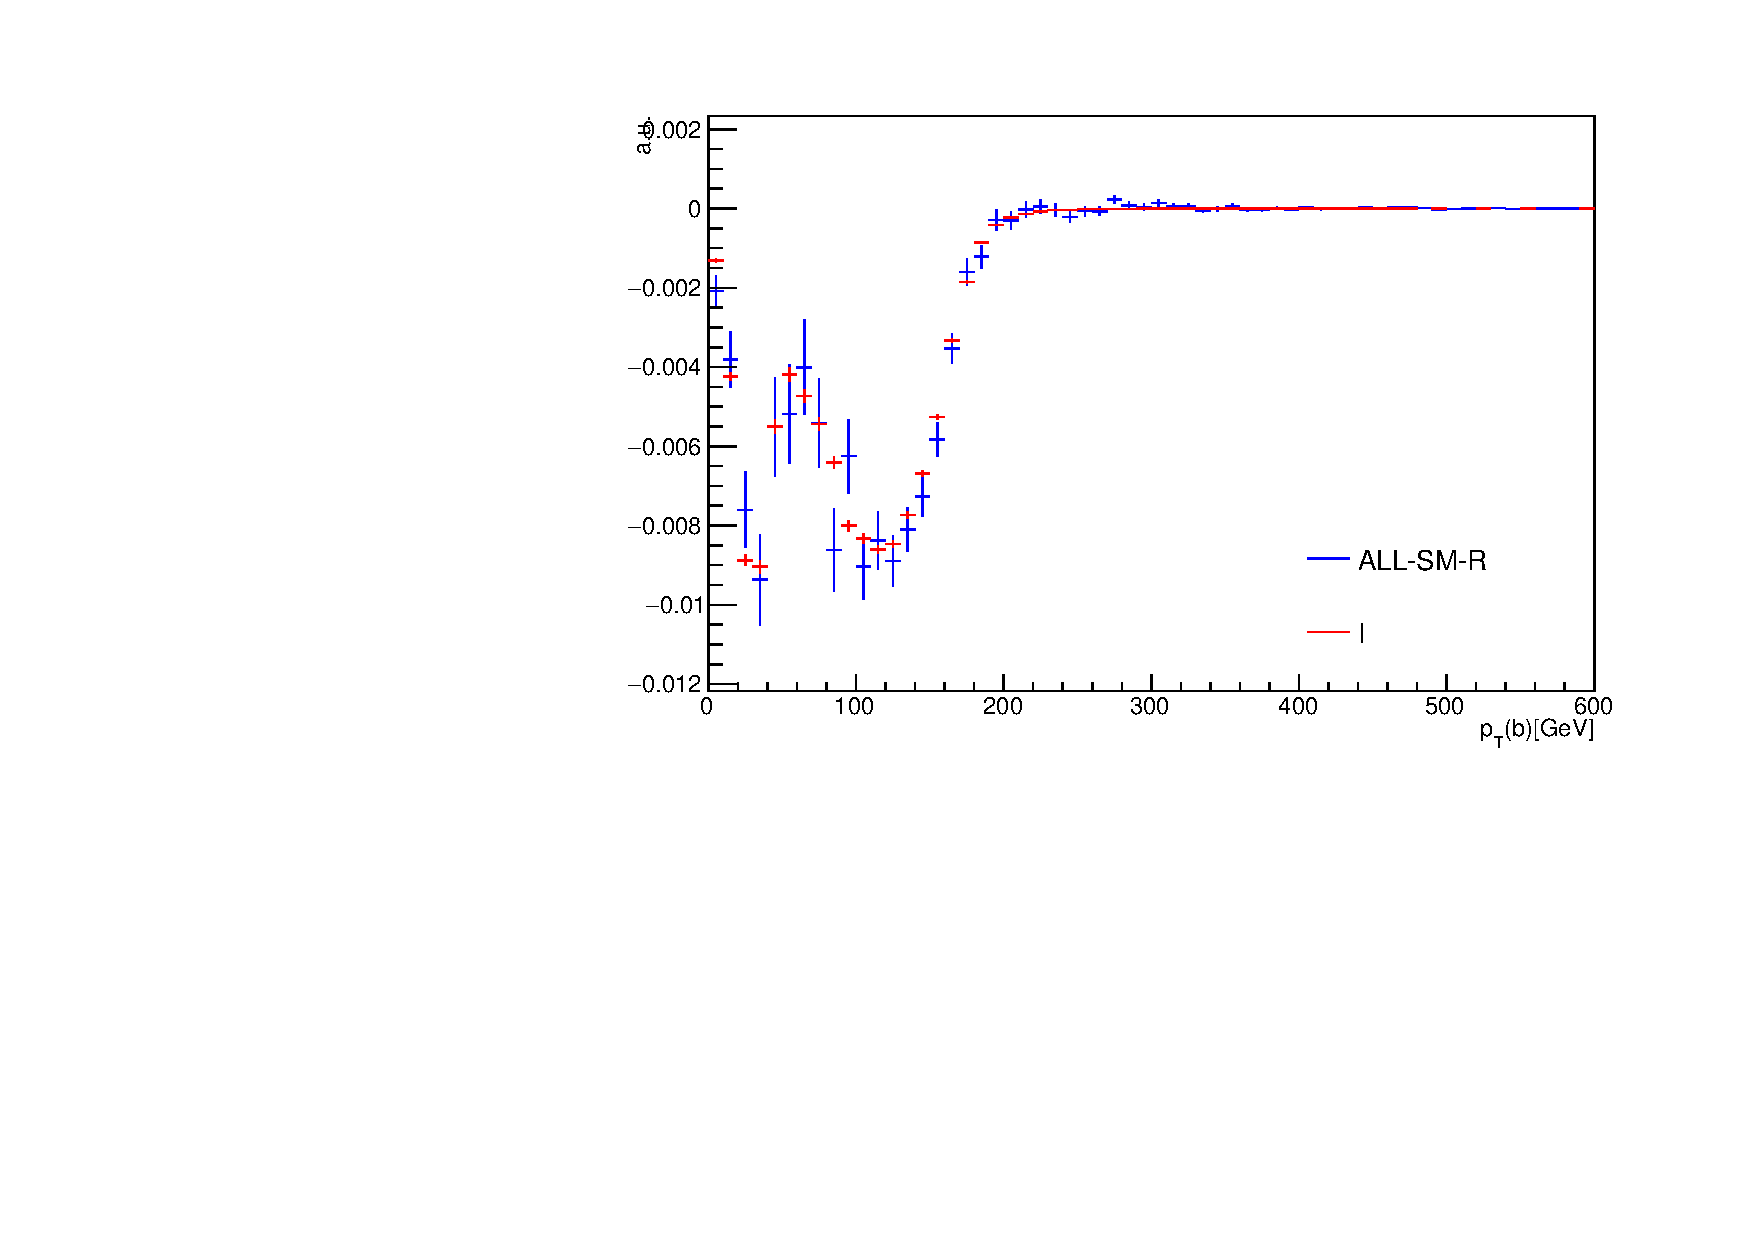
\includegraphics[width=0.4\textwidth]{fig/chapt4/gen_plots/b_pt_compare.pdf}
  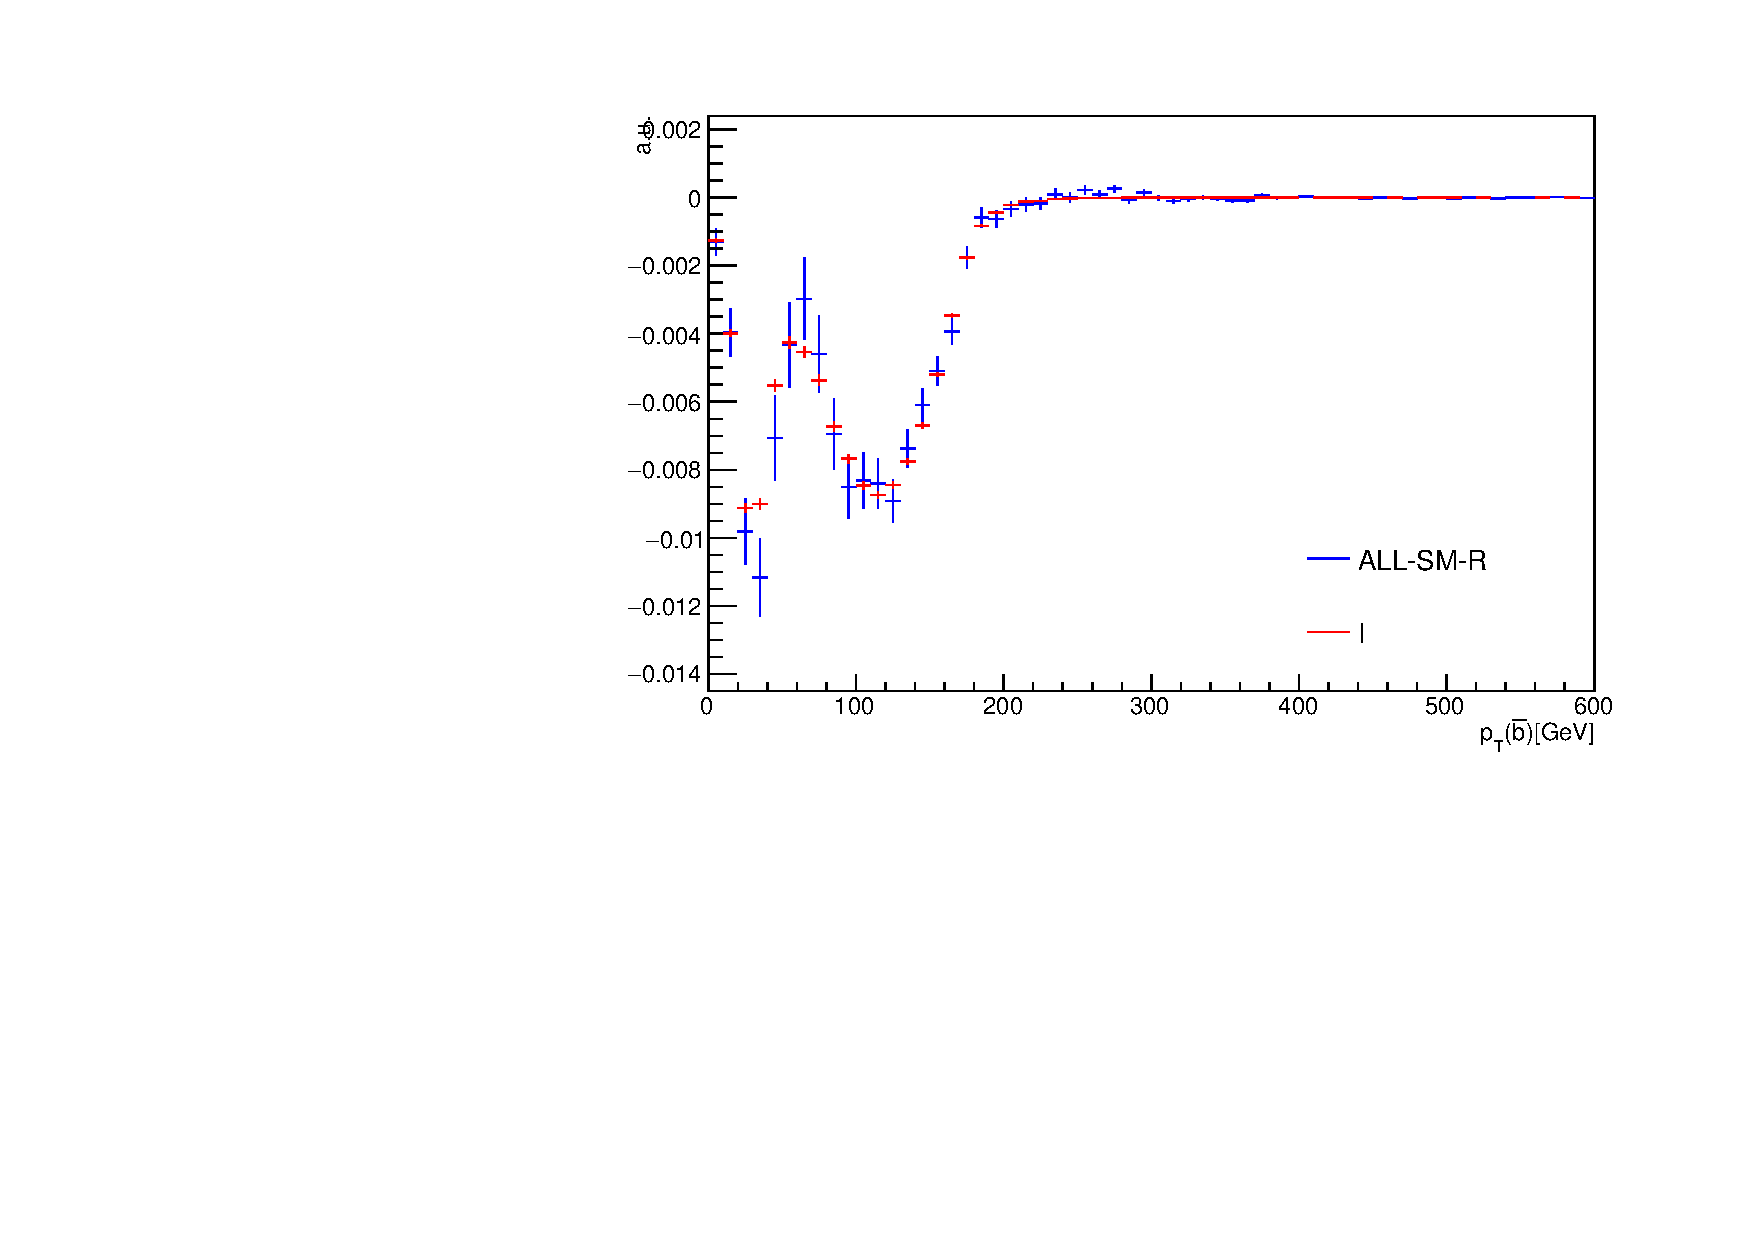
\includegraphics[width=0.4\textwidth]{fig/chapt4/gen_plots/bbar_pt_compare.pdf}\\
  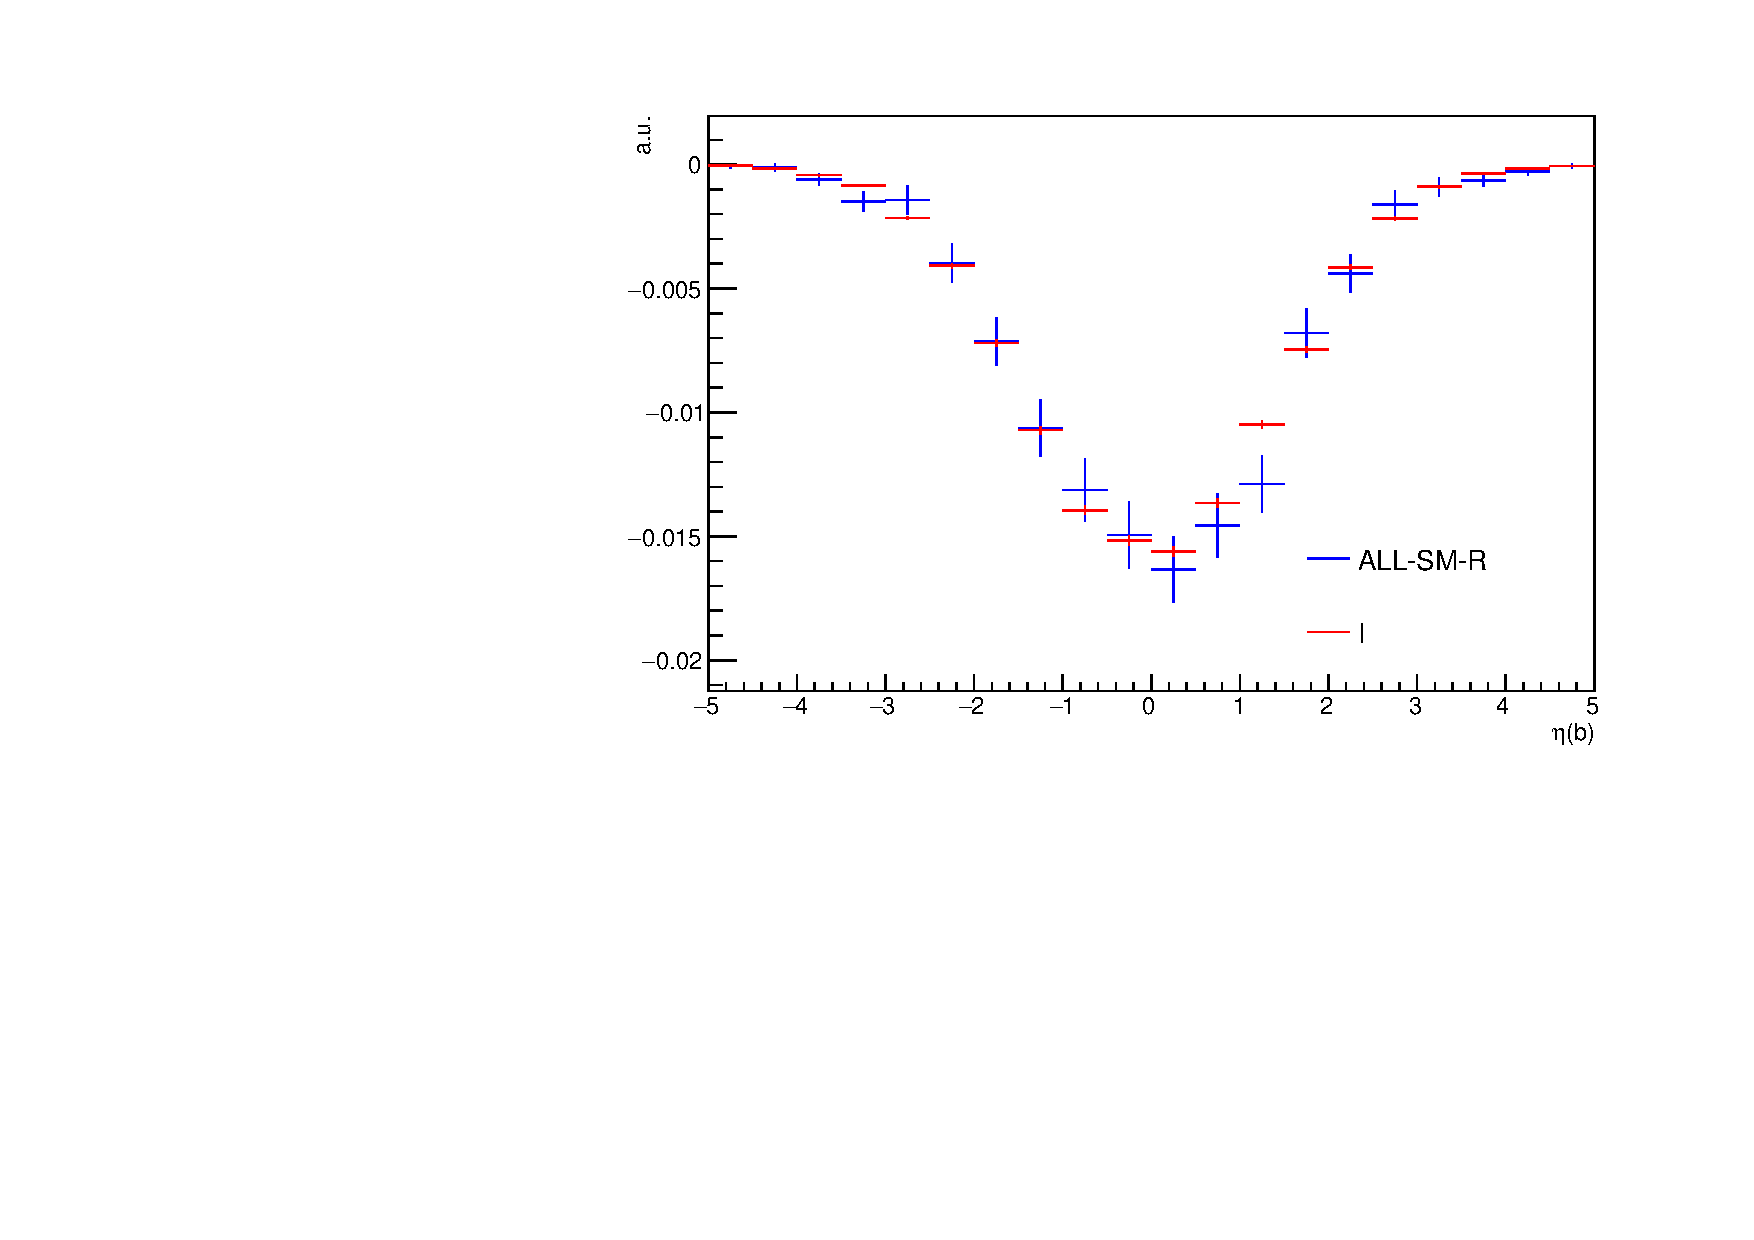
\includegraphics[width=0.4\textwidth]{fig/chapt4/gen_plots/b_eta_compare.pdf}
  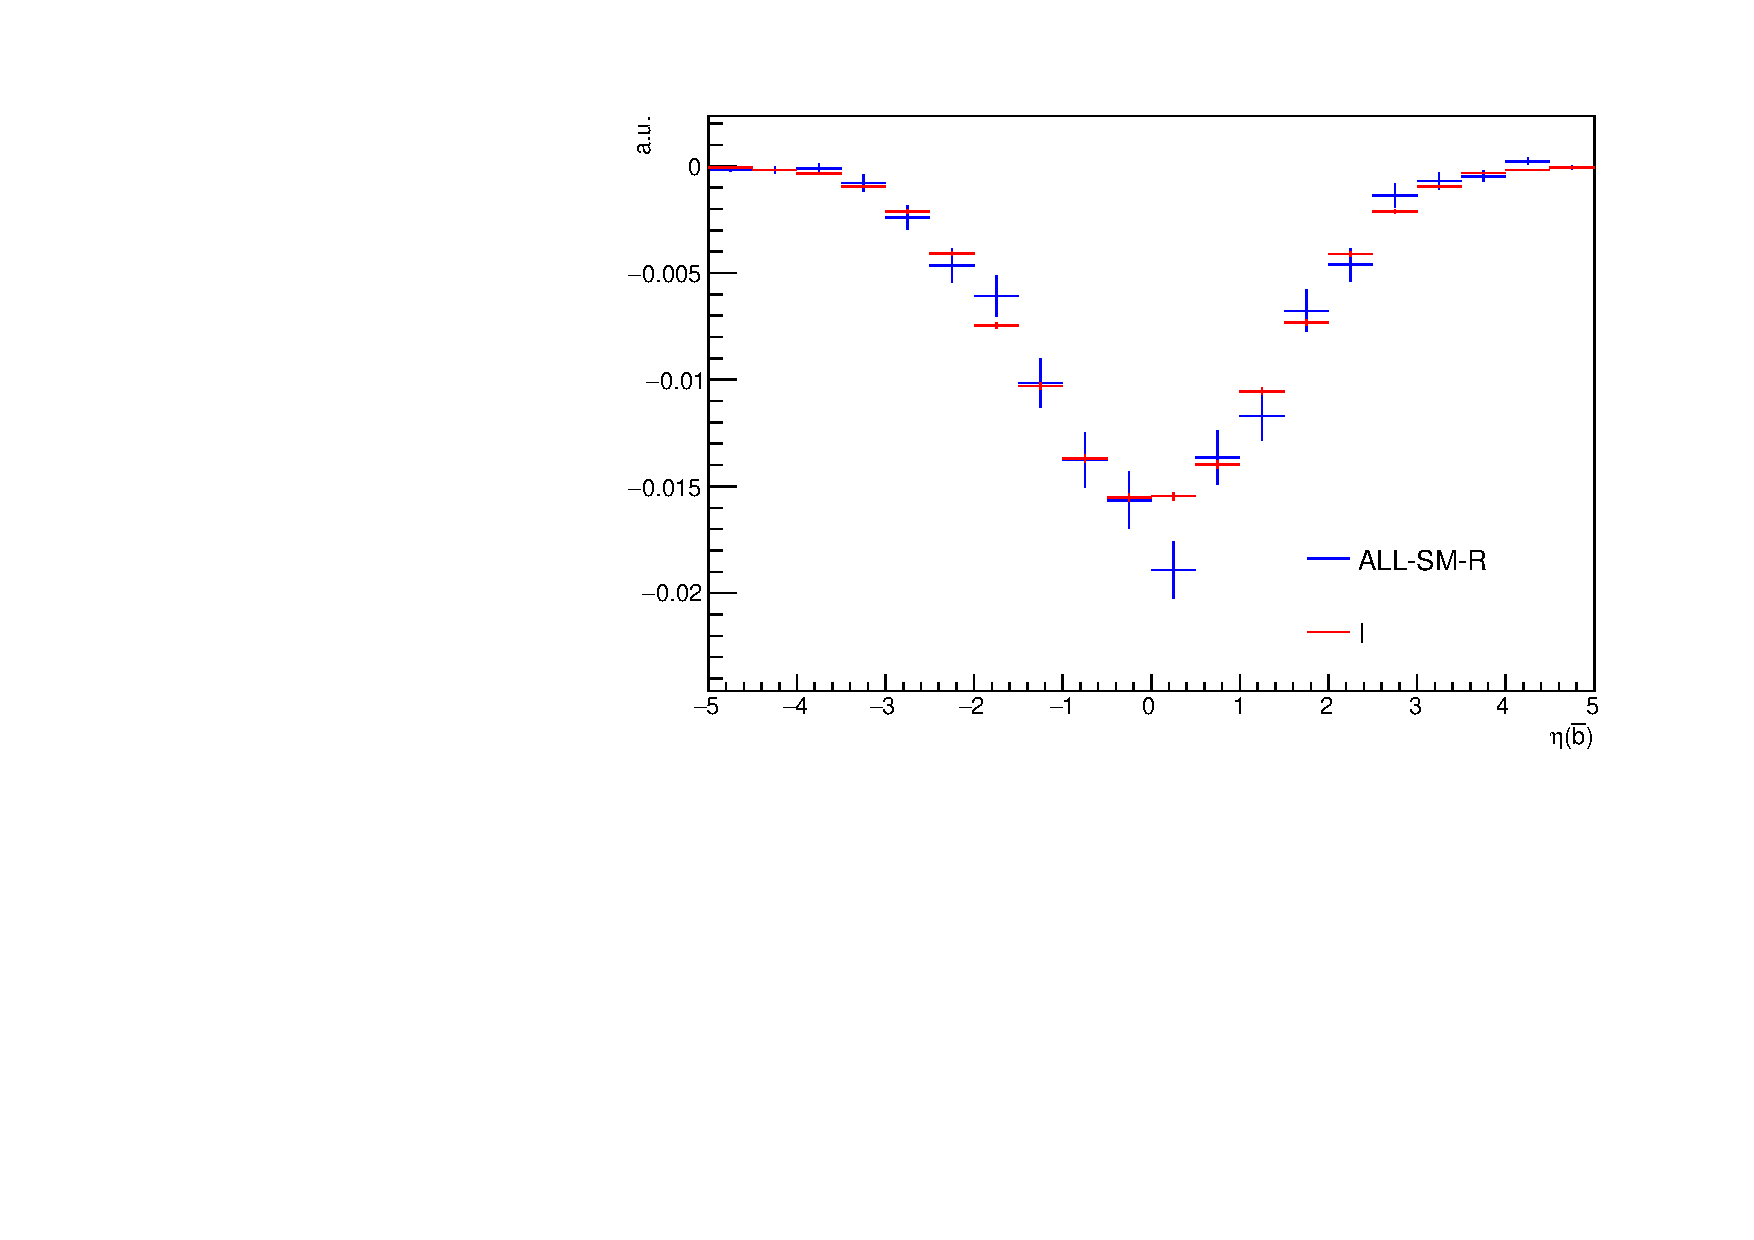
\includegraphics[width=0.4\textwidth]{fig/chapt4/gen_plots/bbar_eta_compare.pdf}\\
  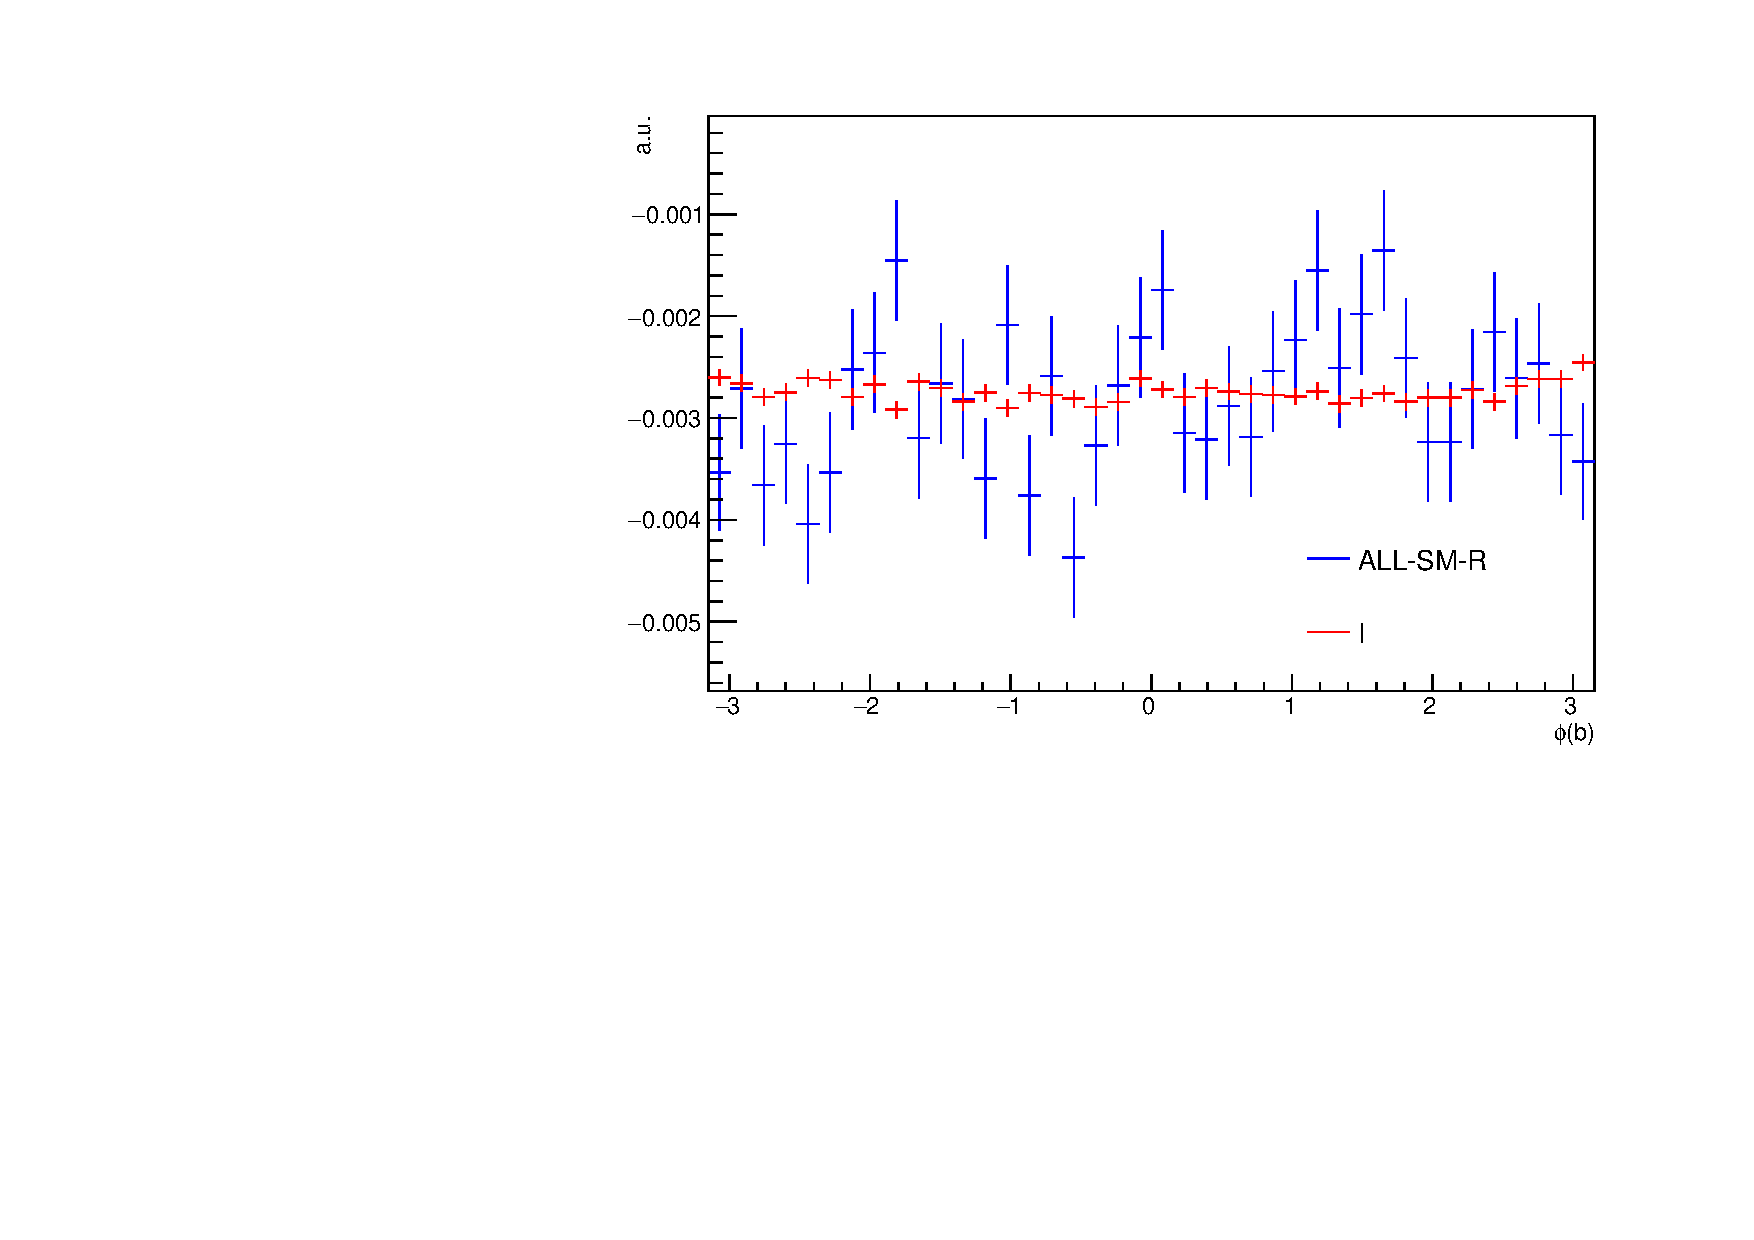
\includegraphics[width=0.4\textwidth]{fig/chapt4/gen_plots/b_phi_compare.pdf}
  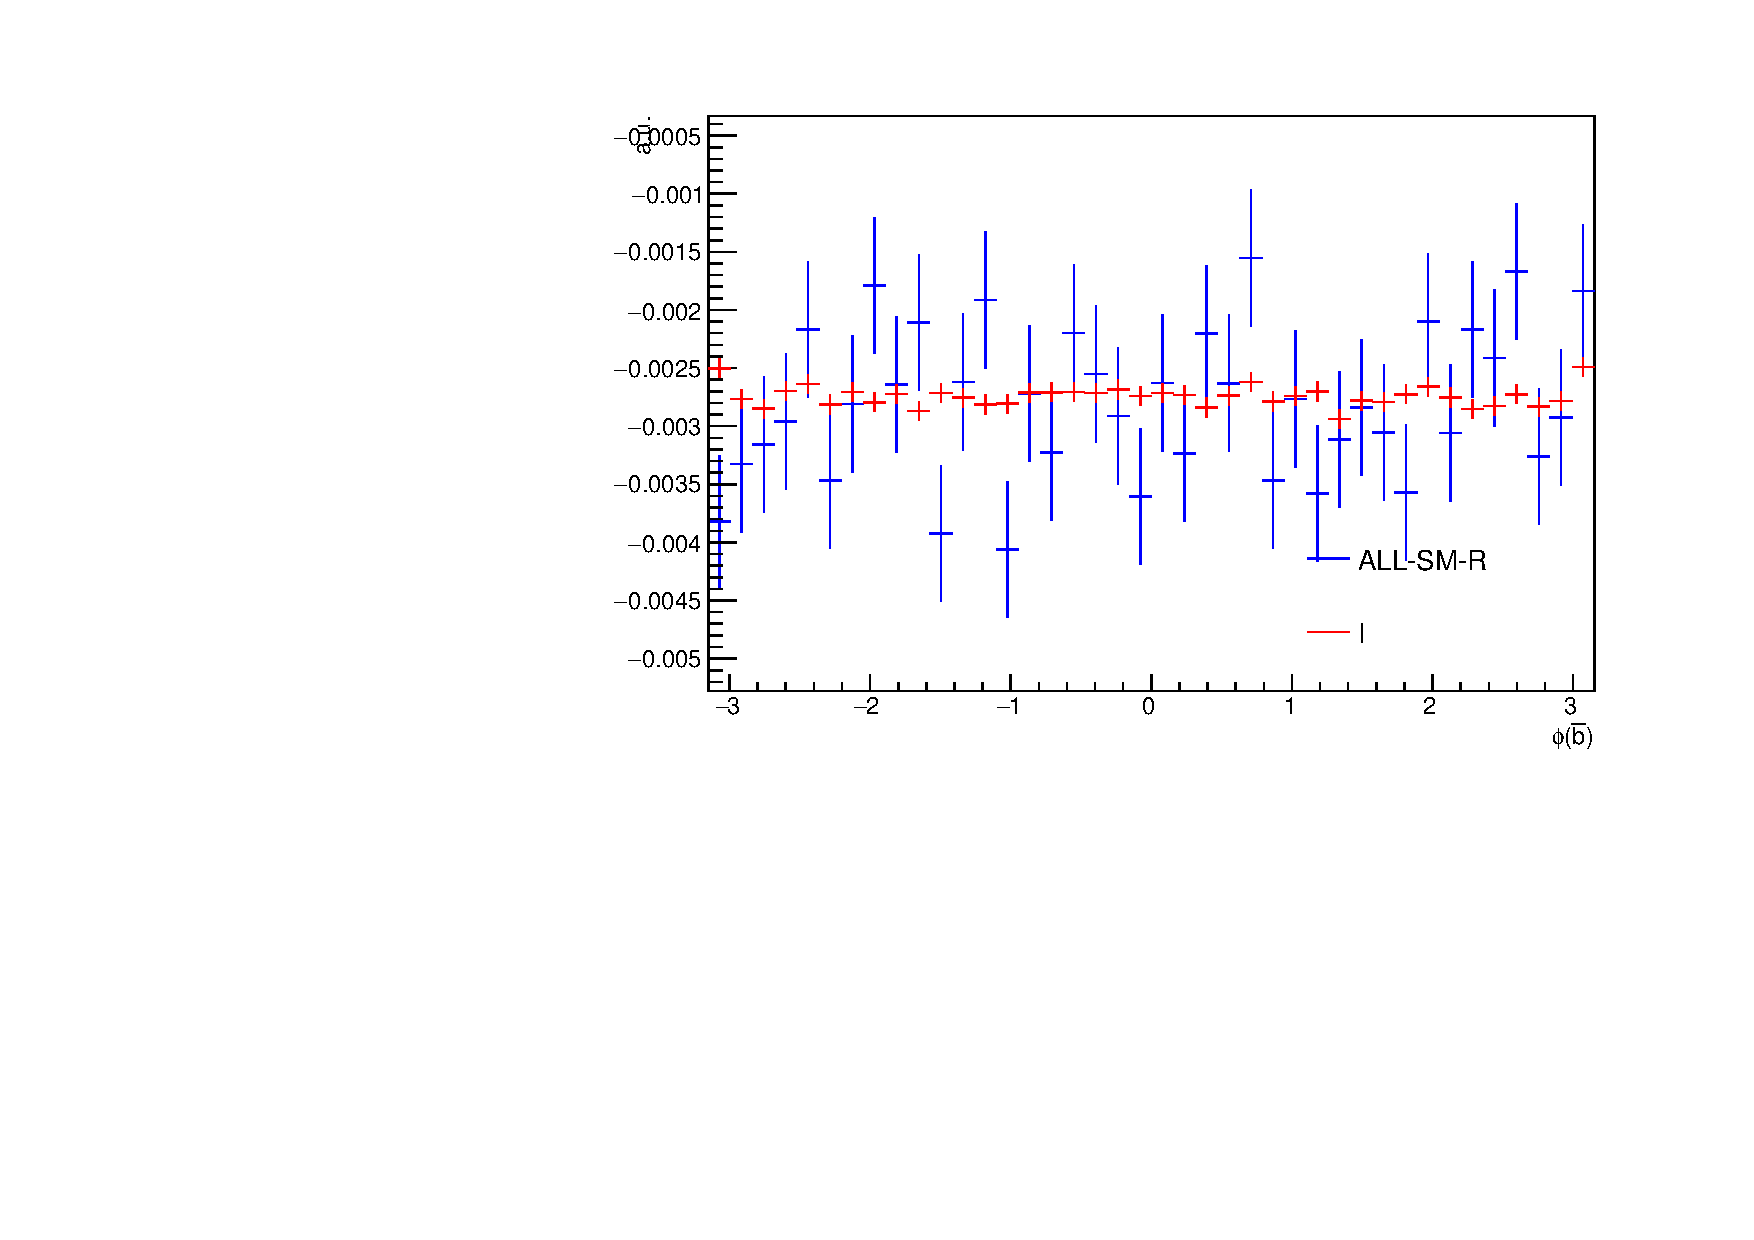
\includegraphics[width=0.4\textwidth]{fig/chapt4/gen_plots/bbar_phi_compare.pdf}
  \caption{Distributions of the transverse momenta, pseudorapidities, and azimuthal angles for bottom quark and antiquark from the decays of the top quarks. Comparison of the two approaches to model the interference.}
  \label{fig:comparison_b}
\end{figure}

\begin{figure} \centering
  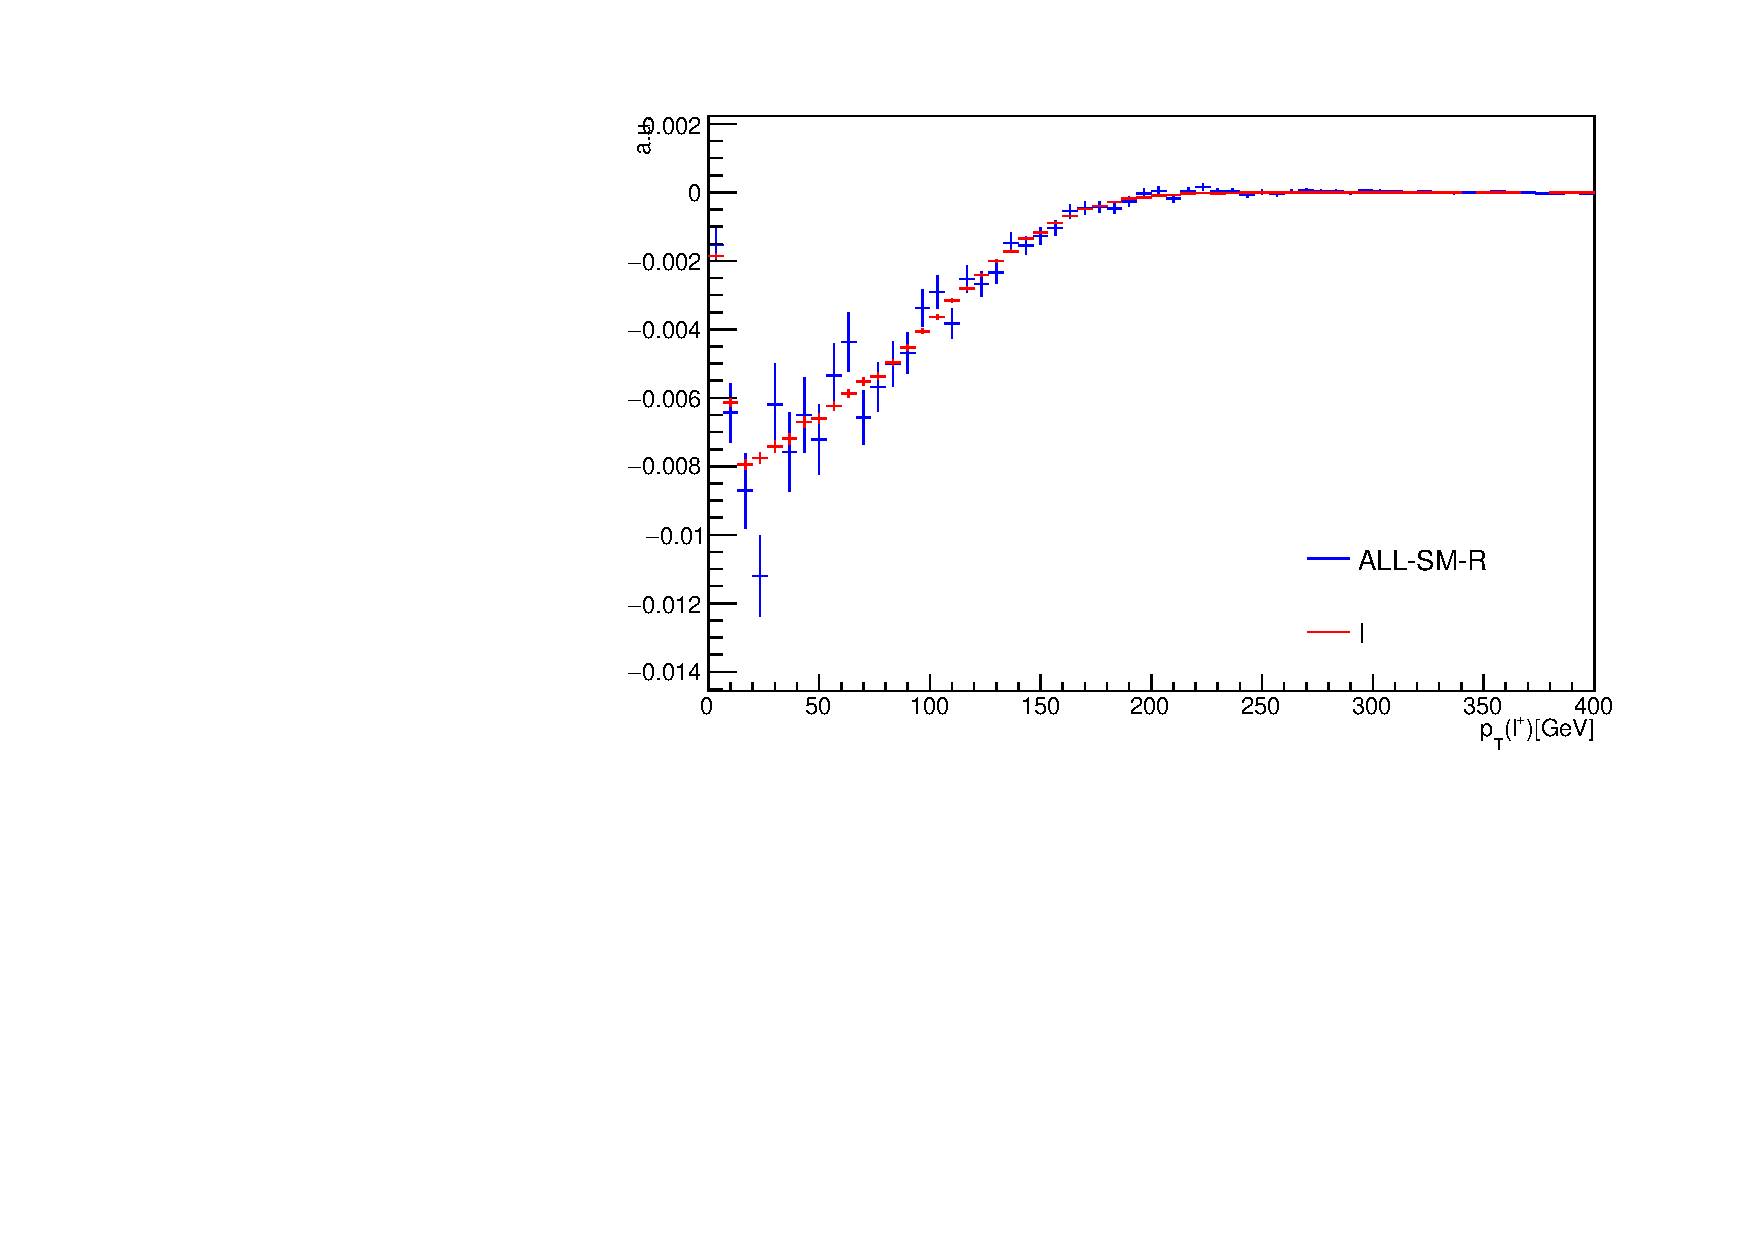
\includegraphics[width=0.4\textwidth]{fig/chapt4/gen_plots/lplus_pt_compare.pdf}
  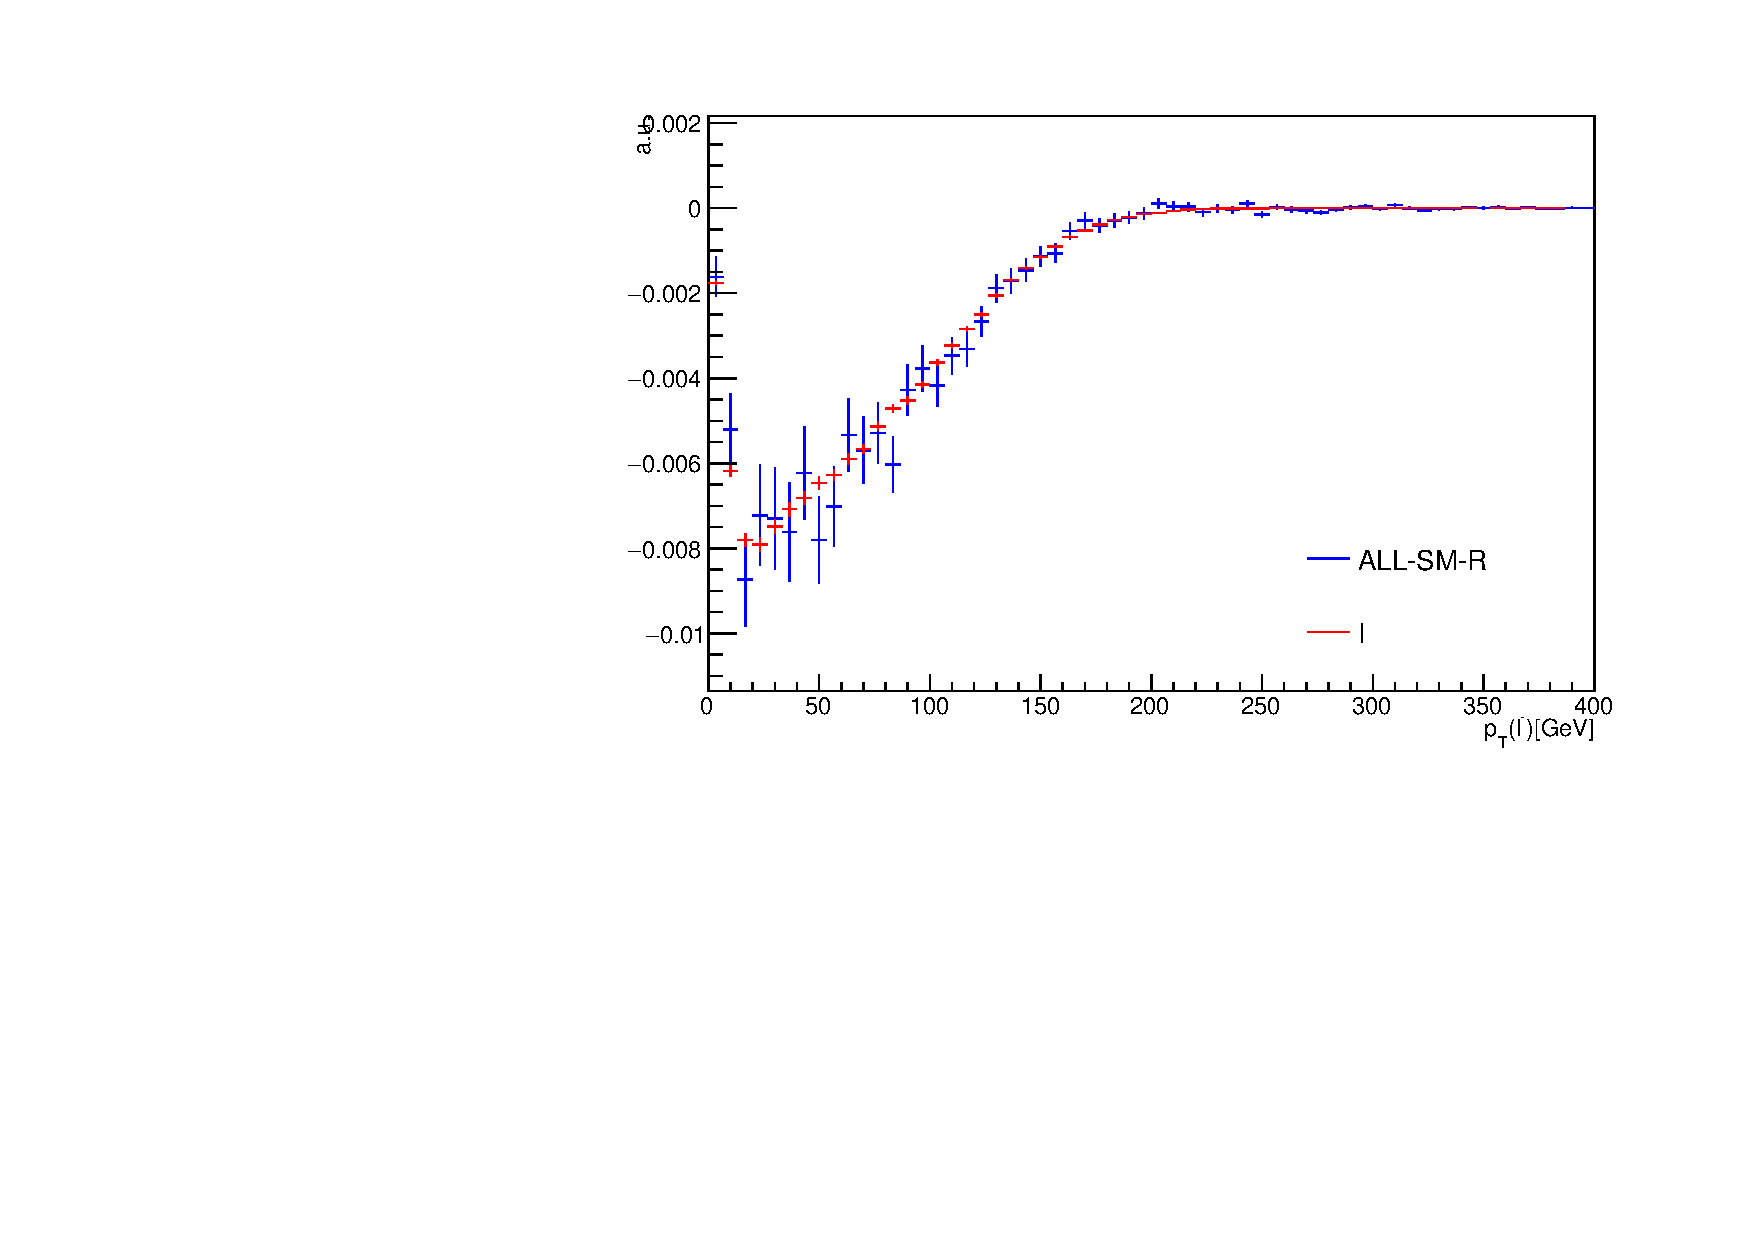
\includegraphics[width=0.4\textwidth]{fig/chapt4/gen_plots/lminus_pt_compare.pdf}\\
  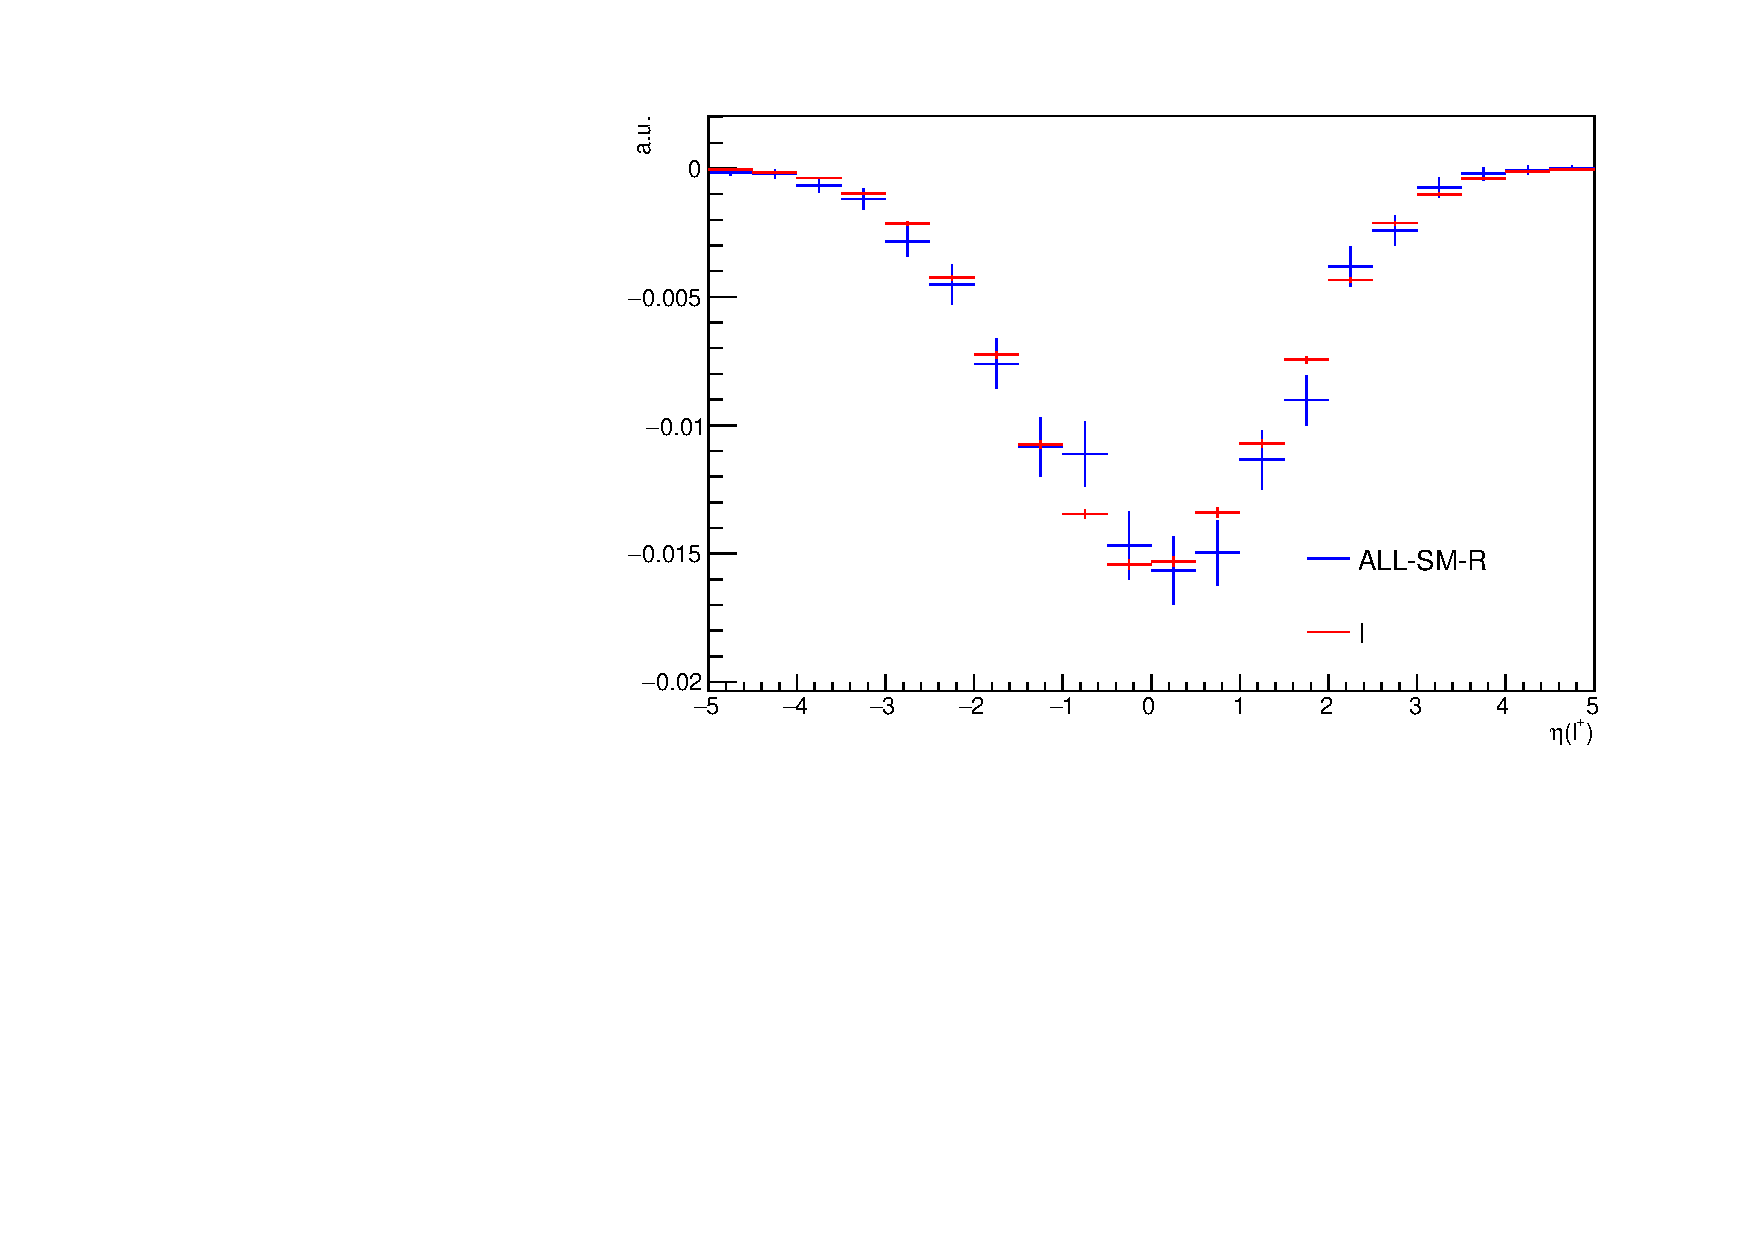
\includegraphics[width=0.4\textwidth]{fig/chapt4/gen_plots/lplus_eta_compare.pdf}
  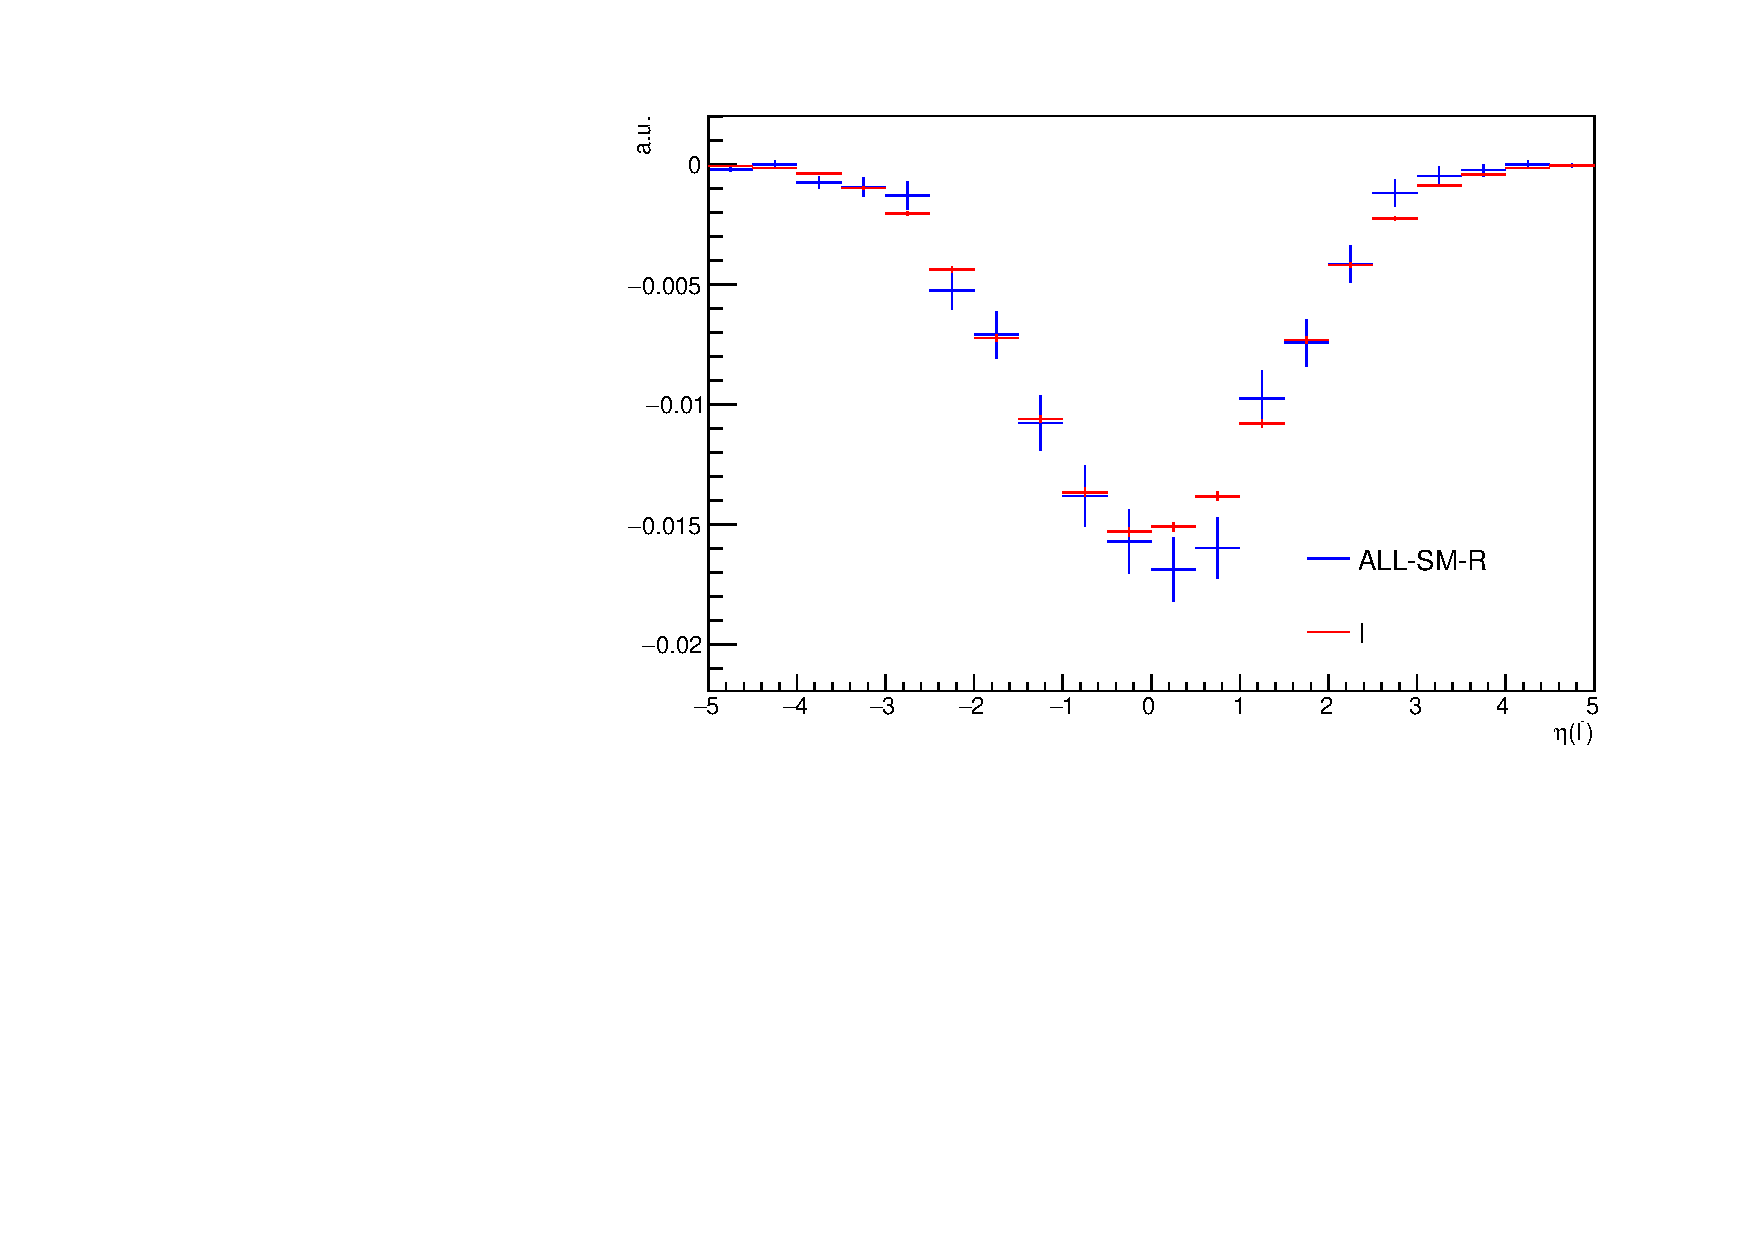
\includegraphics[width=0.4\textwidth]{fig/chapt4/gen_plots/lminus_eta_compare.pdf}\\
  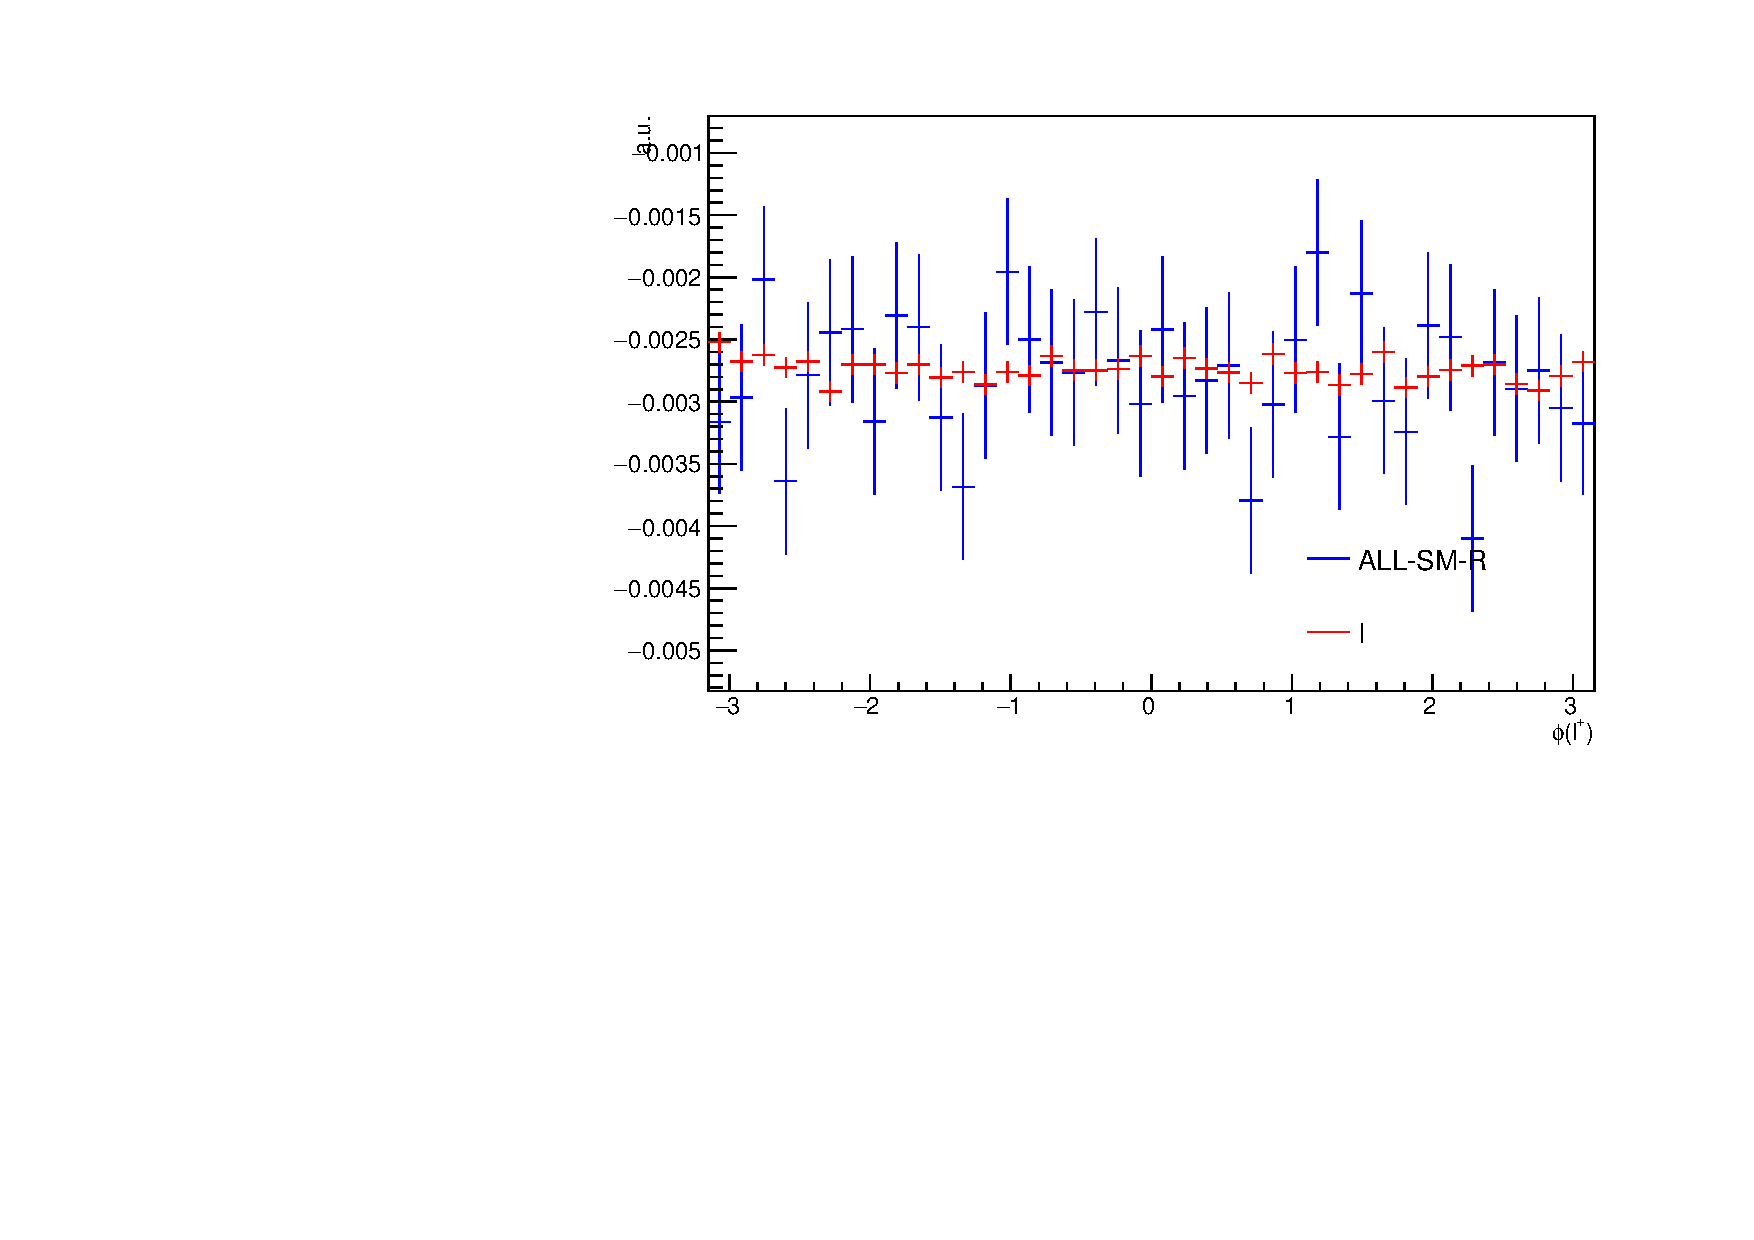
\includegraphics[width=0.4\textwidth]{fig/chapt4/gen_plots/lplus_phi_compare.pdf}
  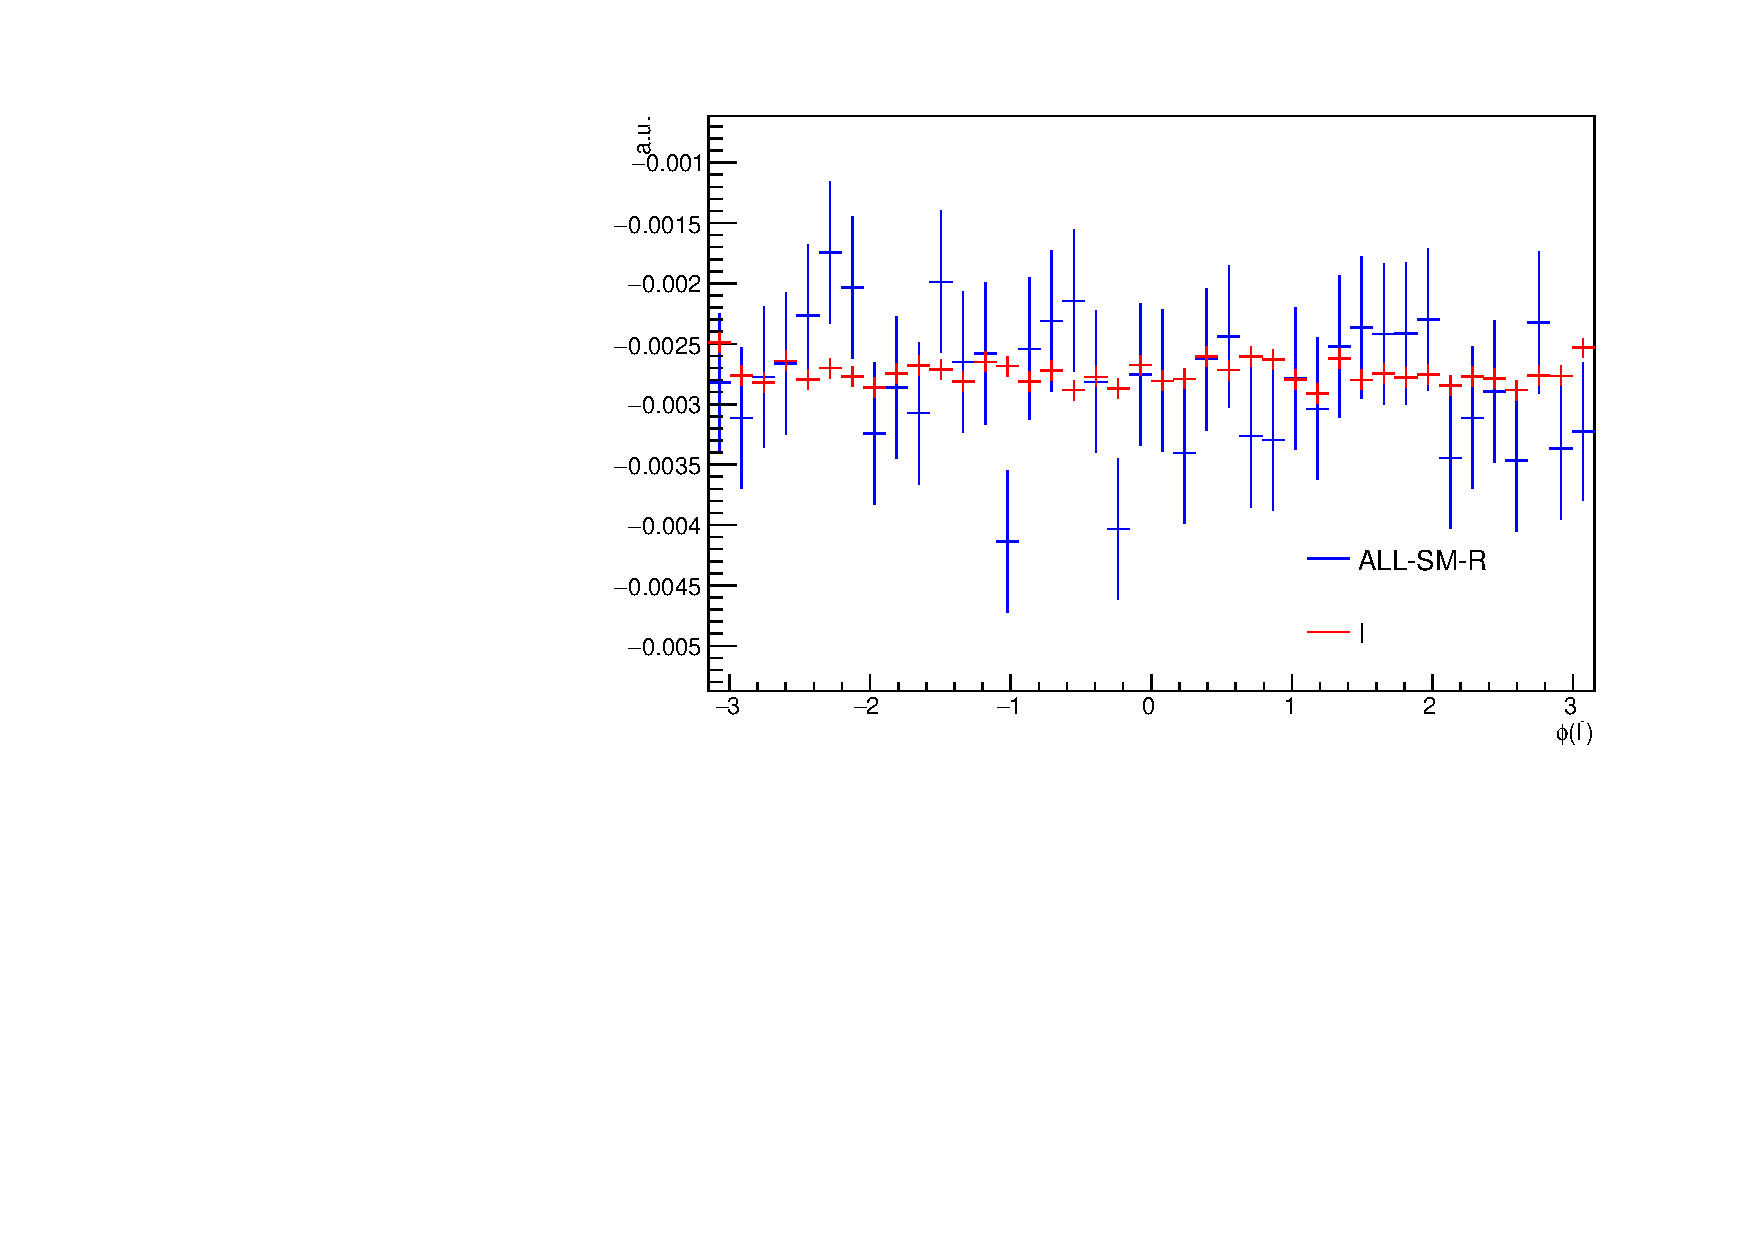
\includegraphics[width=0.4\textwidth]{fig/chapt4/gen_plots/lminus_phi_compare.pdf}
  \caption{Distributions of the transverse momenta, pseudorapidities, and azimuthal angles for changed leptons stemming from the decays of the top quarks. Comparison of the two approaches to model the interference.}
  \label{fig:comparison_leptons}
\end{figure}

\begin{figure} \centering
  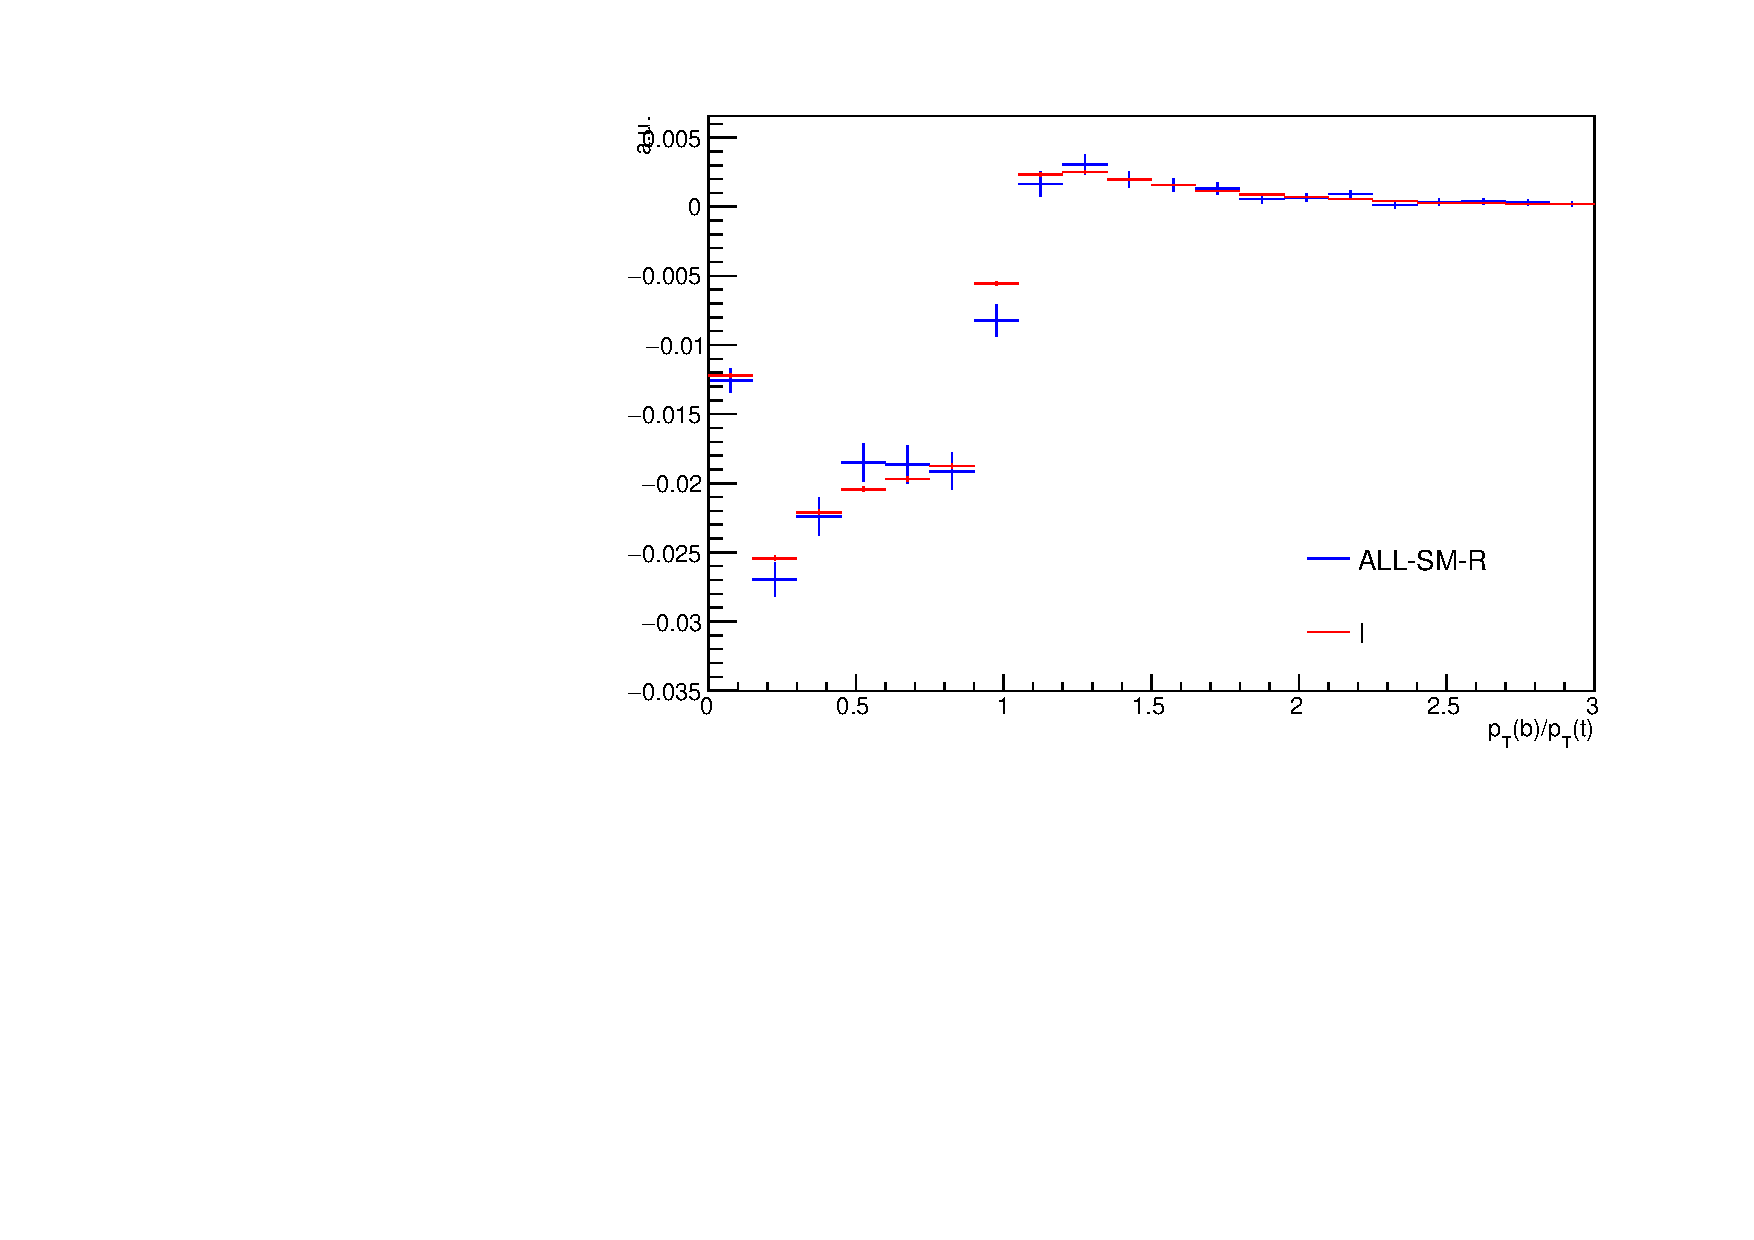
\includegraphics[width=0.4\textwidth]{fig/chapt4/gen_plots/b_over_t_pt_compare.pdf}
  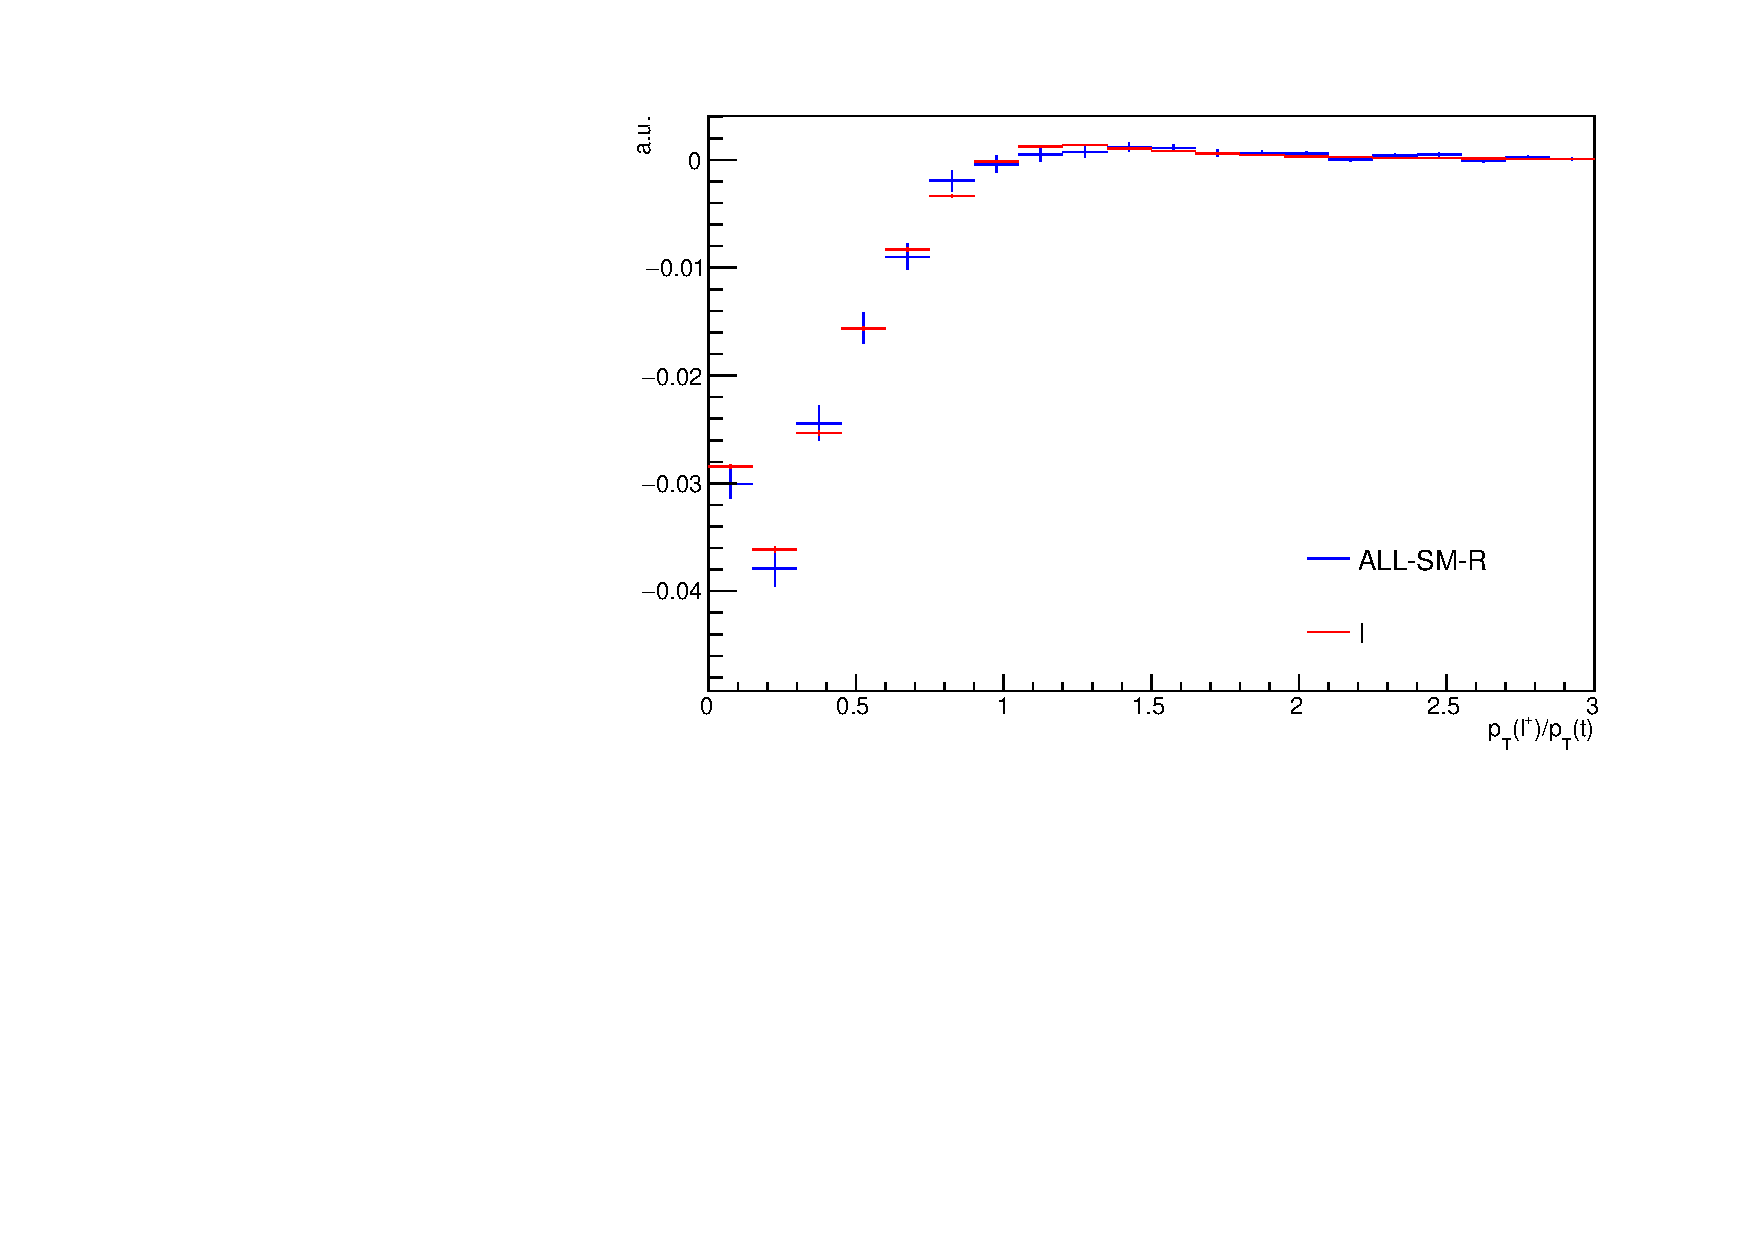
\includegraphics[width=0.4\textwidth]{fig/chapt4/gen_plots/lp_over_t_pt_compare.pdf}\\
  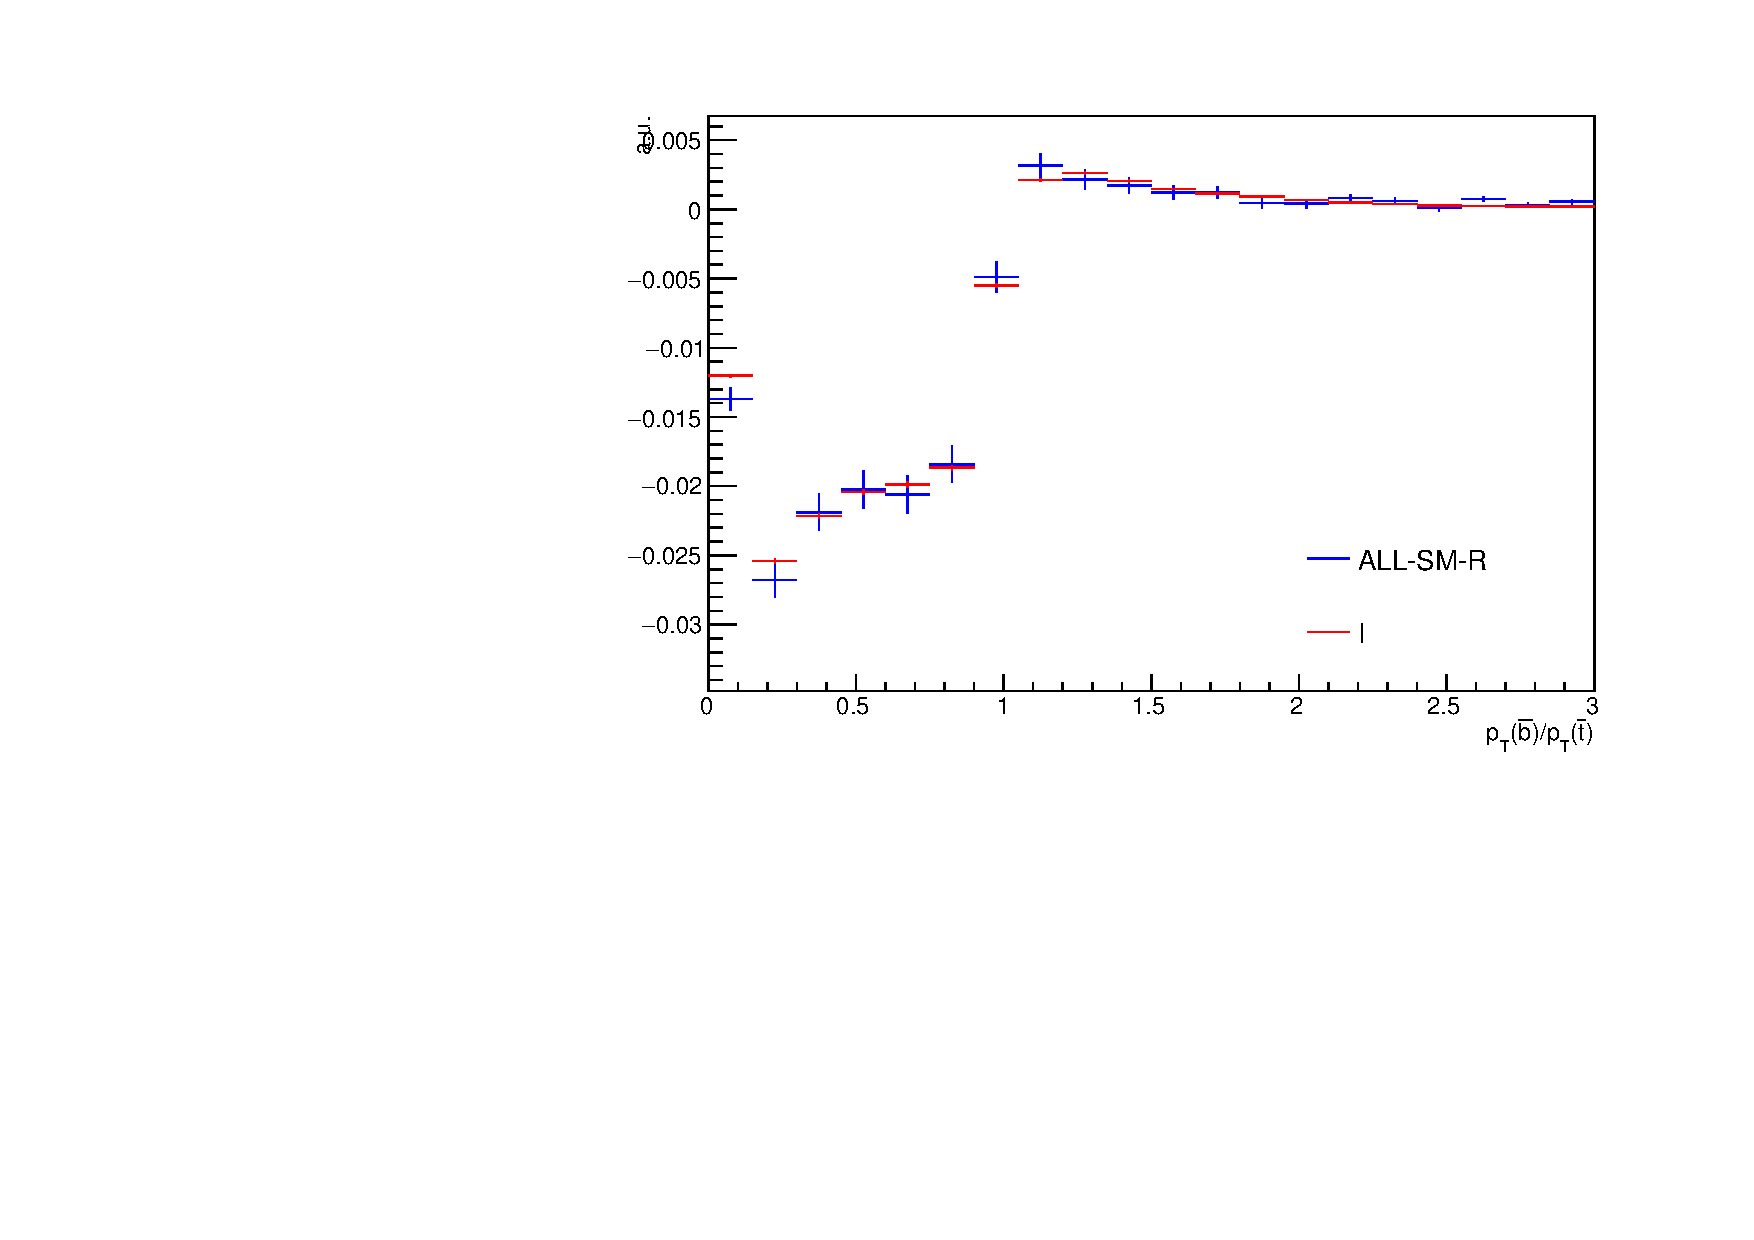
\includegraphics[width=0.4\textwidth]{fig/chapt4/gen_plots/bbar_over_tbar_pt_compare.pdf}
  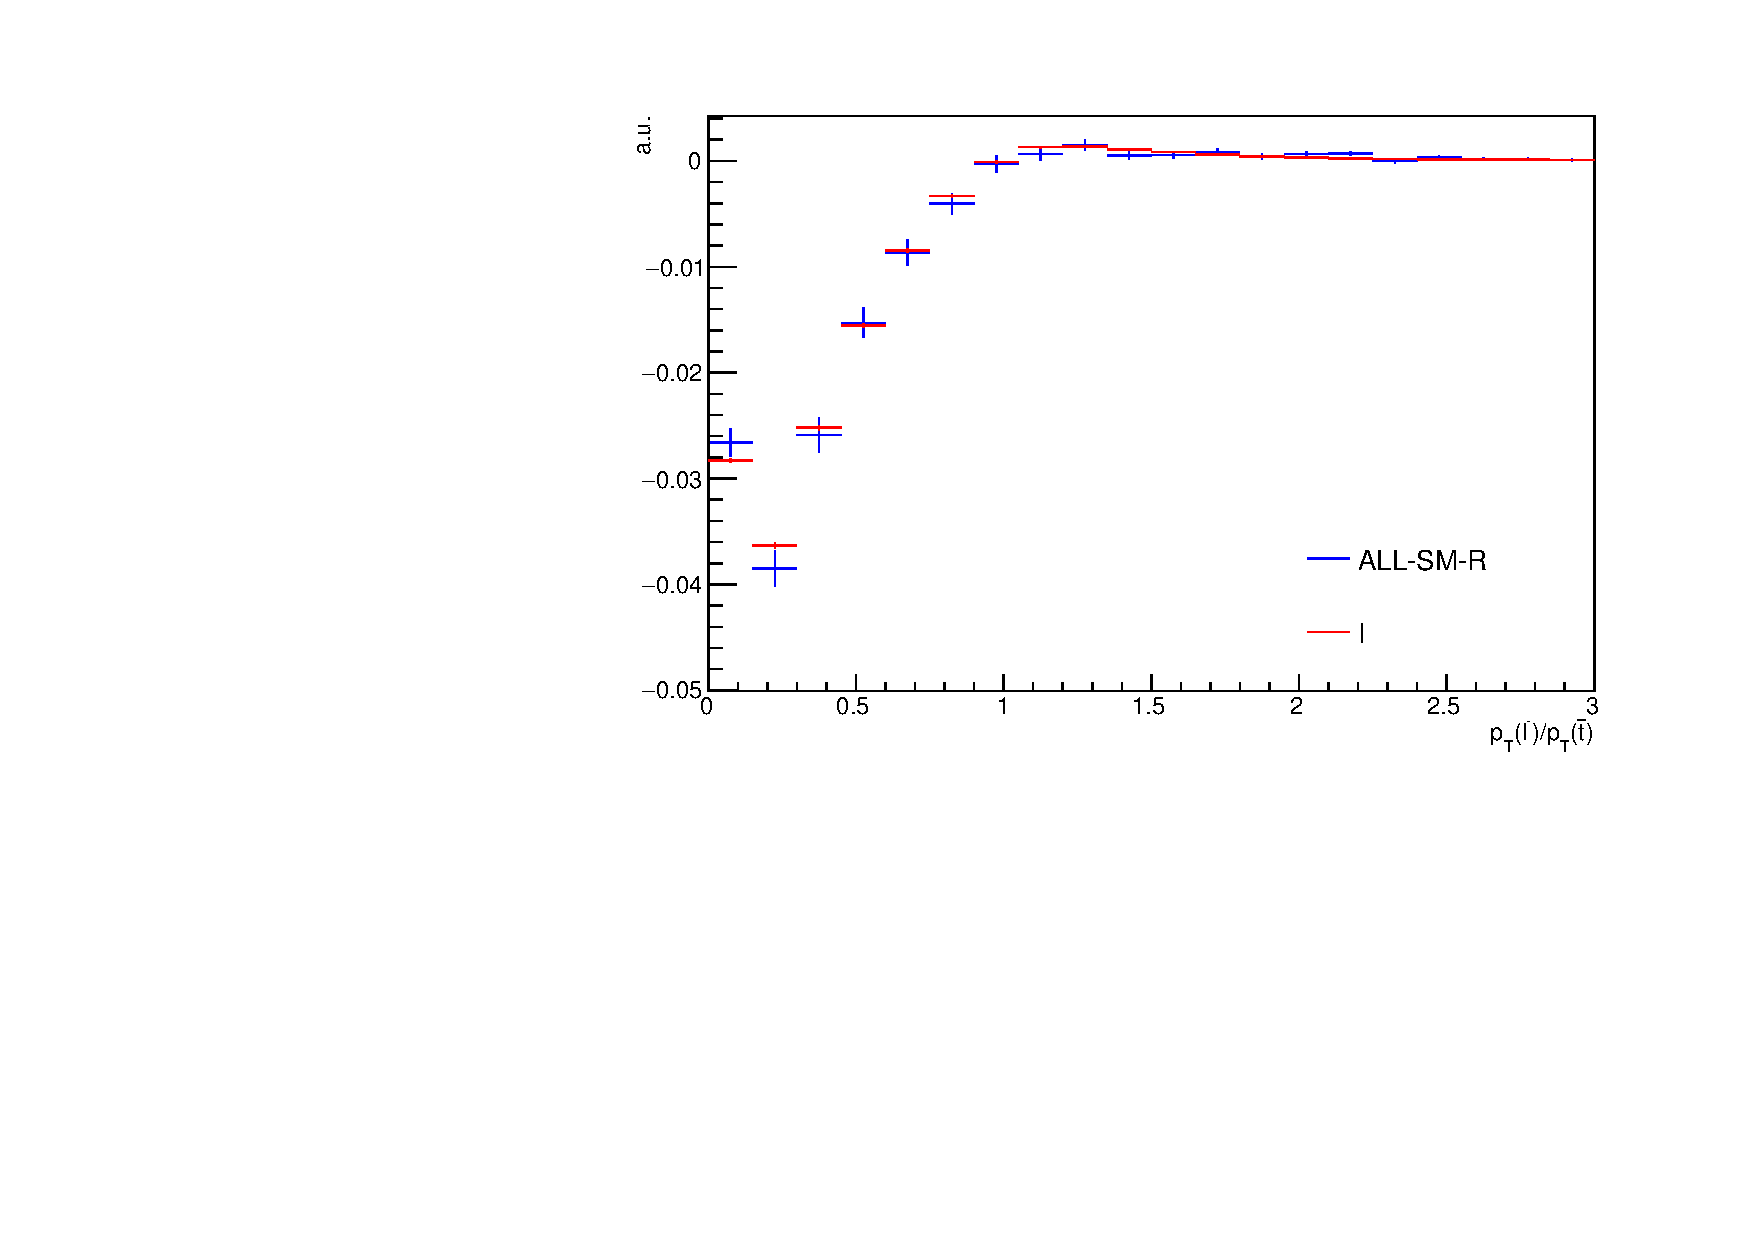
\includegraphics[width=0.4\textwidth]{fig/chapt4/gen_plots/lm_over_tbar_pt_compare.pdf}\\
  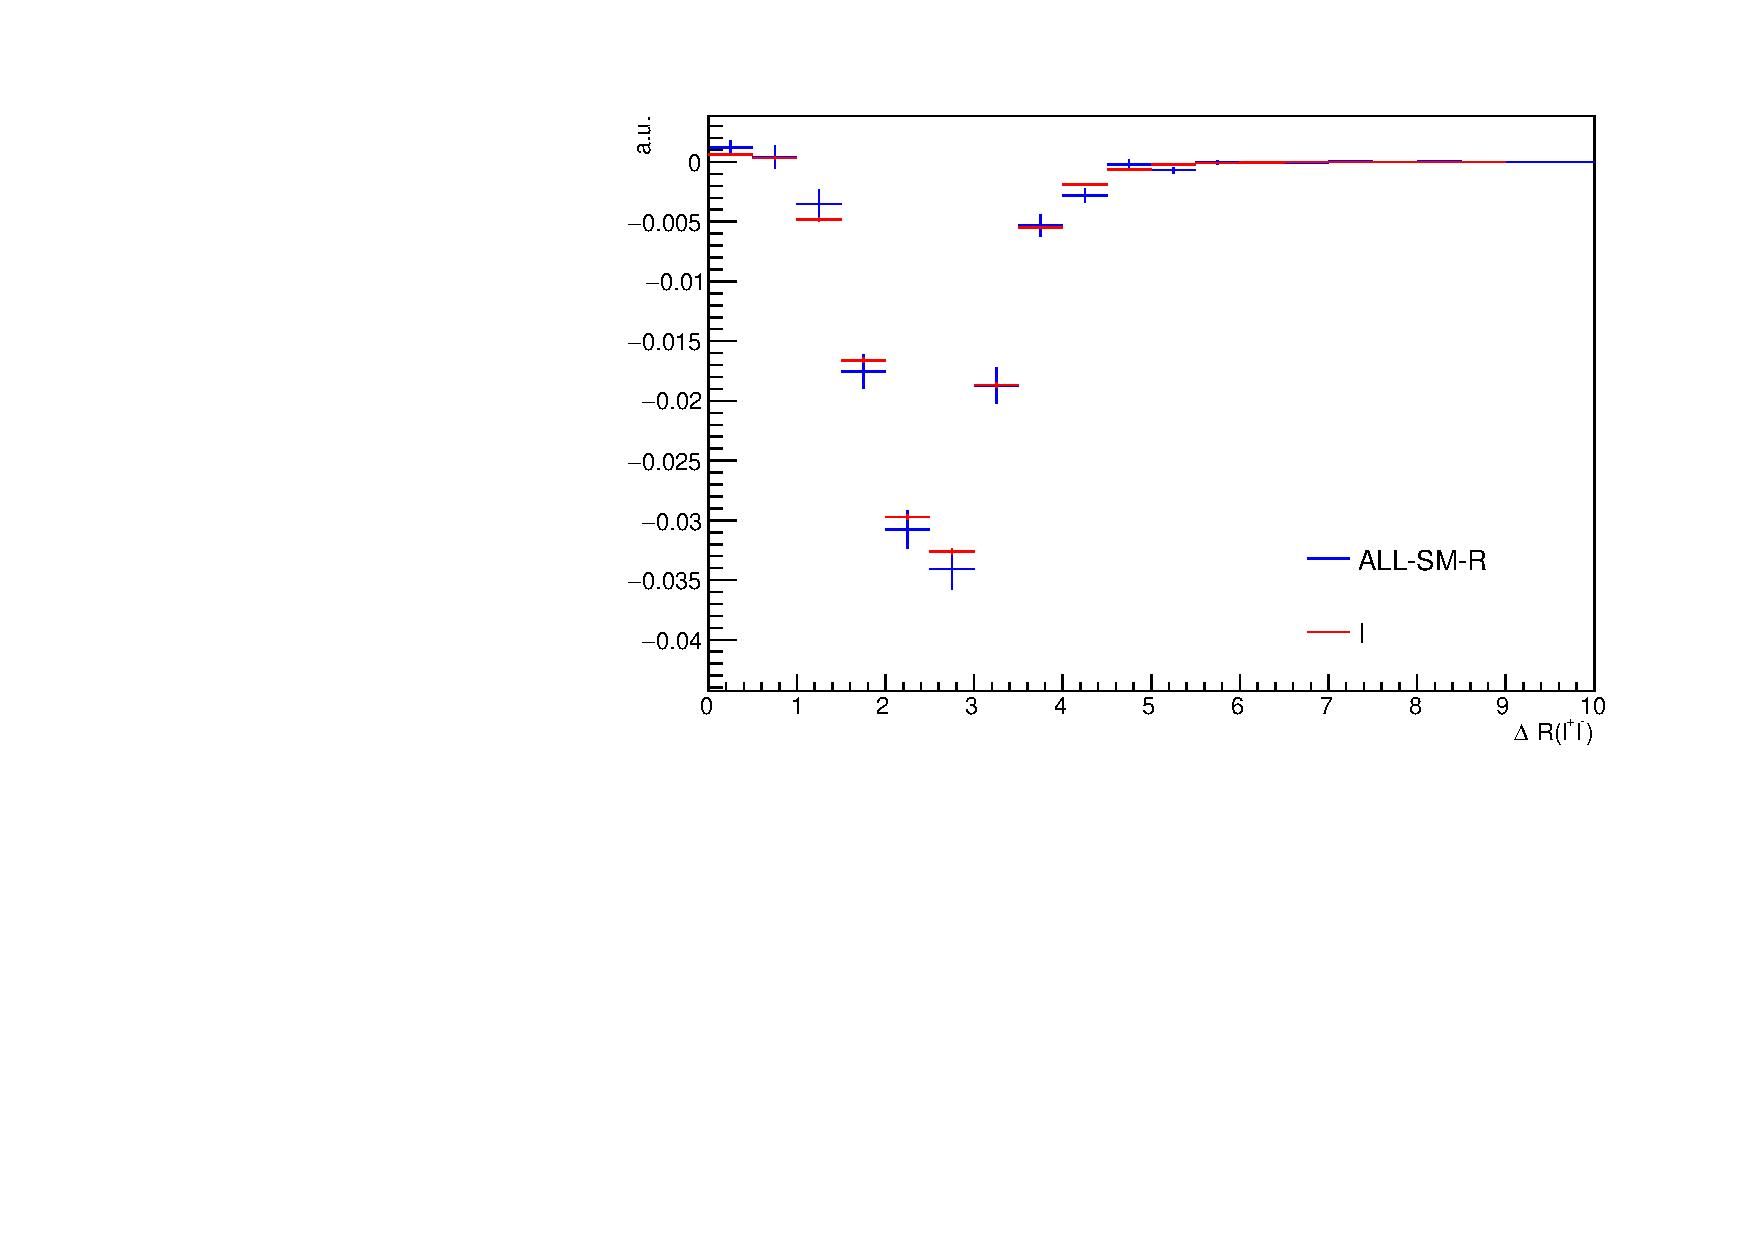
\includegraphics[width=0.4\textwidth]{fig/chapt4/gen_plots/ll_deltaR_compare.pdf}
  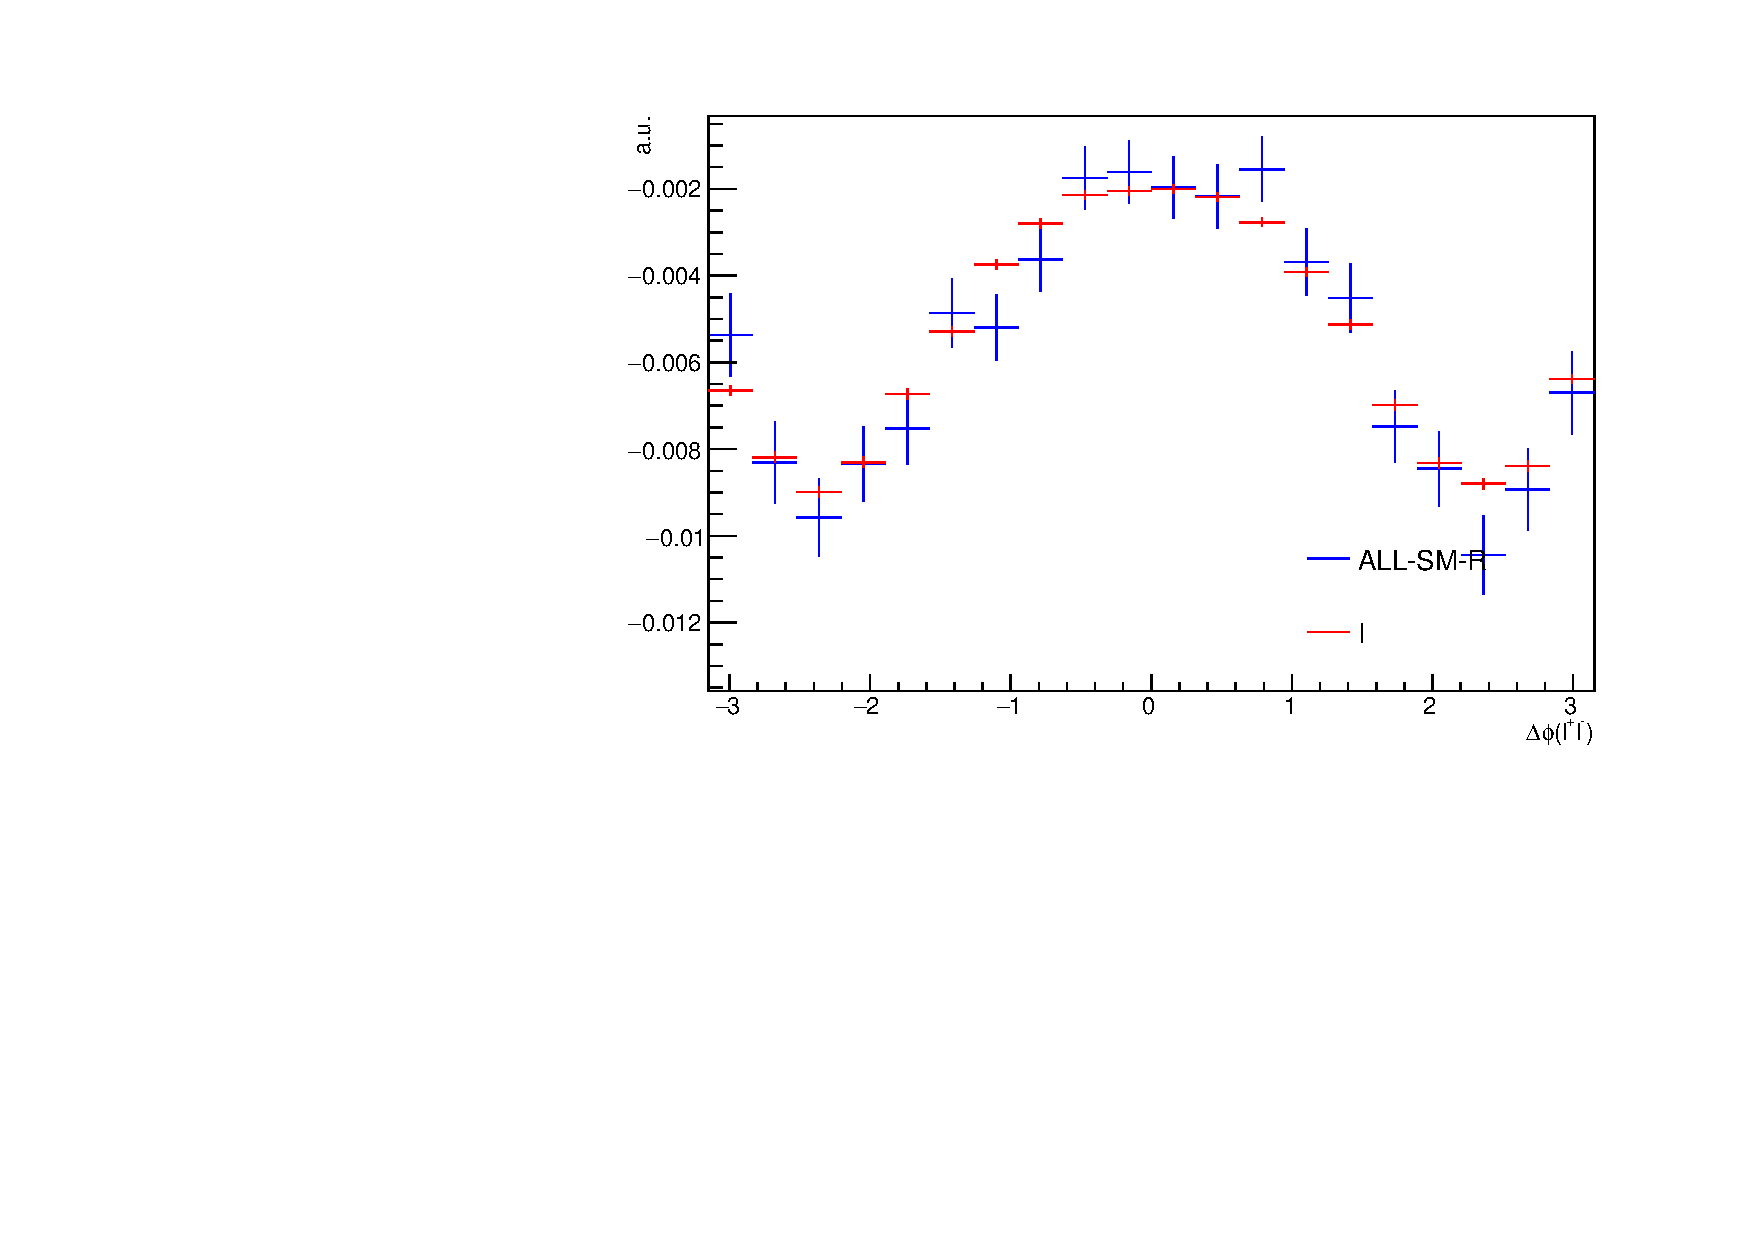
\includegraphics[width=0.4\textwidth]{fig/chapt4/gen_plots/ll_deltaphi_compare.pdf}
  \caption{Distributions of the fractions of the top quark's transverse momentum carried by the b~quark and the charged lepton from its decay (top), the similar fractions from top antiquark (middle), and the $\Delta R$ and $\Delta\phi$ distances between the two leptons (bottom). Comparison of the two approaches to model the interference.}
  \label{fig:comparison_bandl_relto_top}
\end{figure}

\begin{figure} \centering
  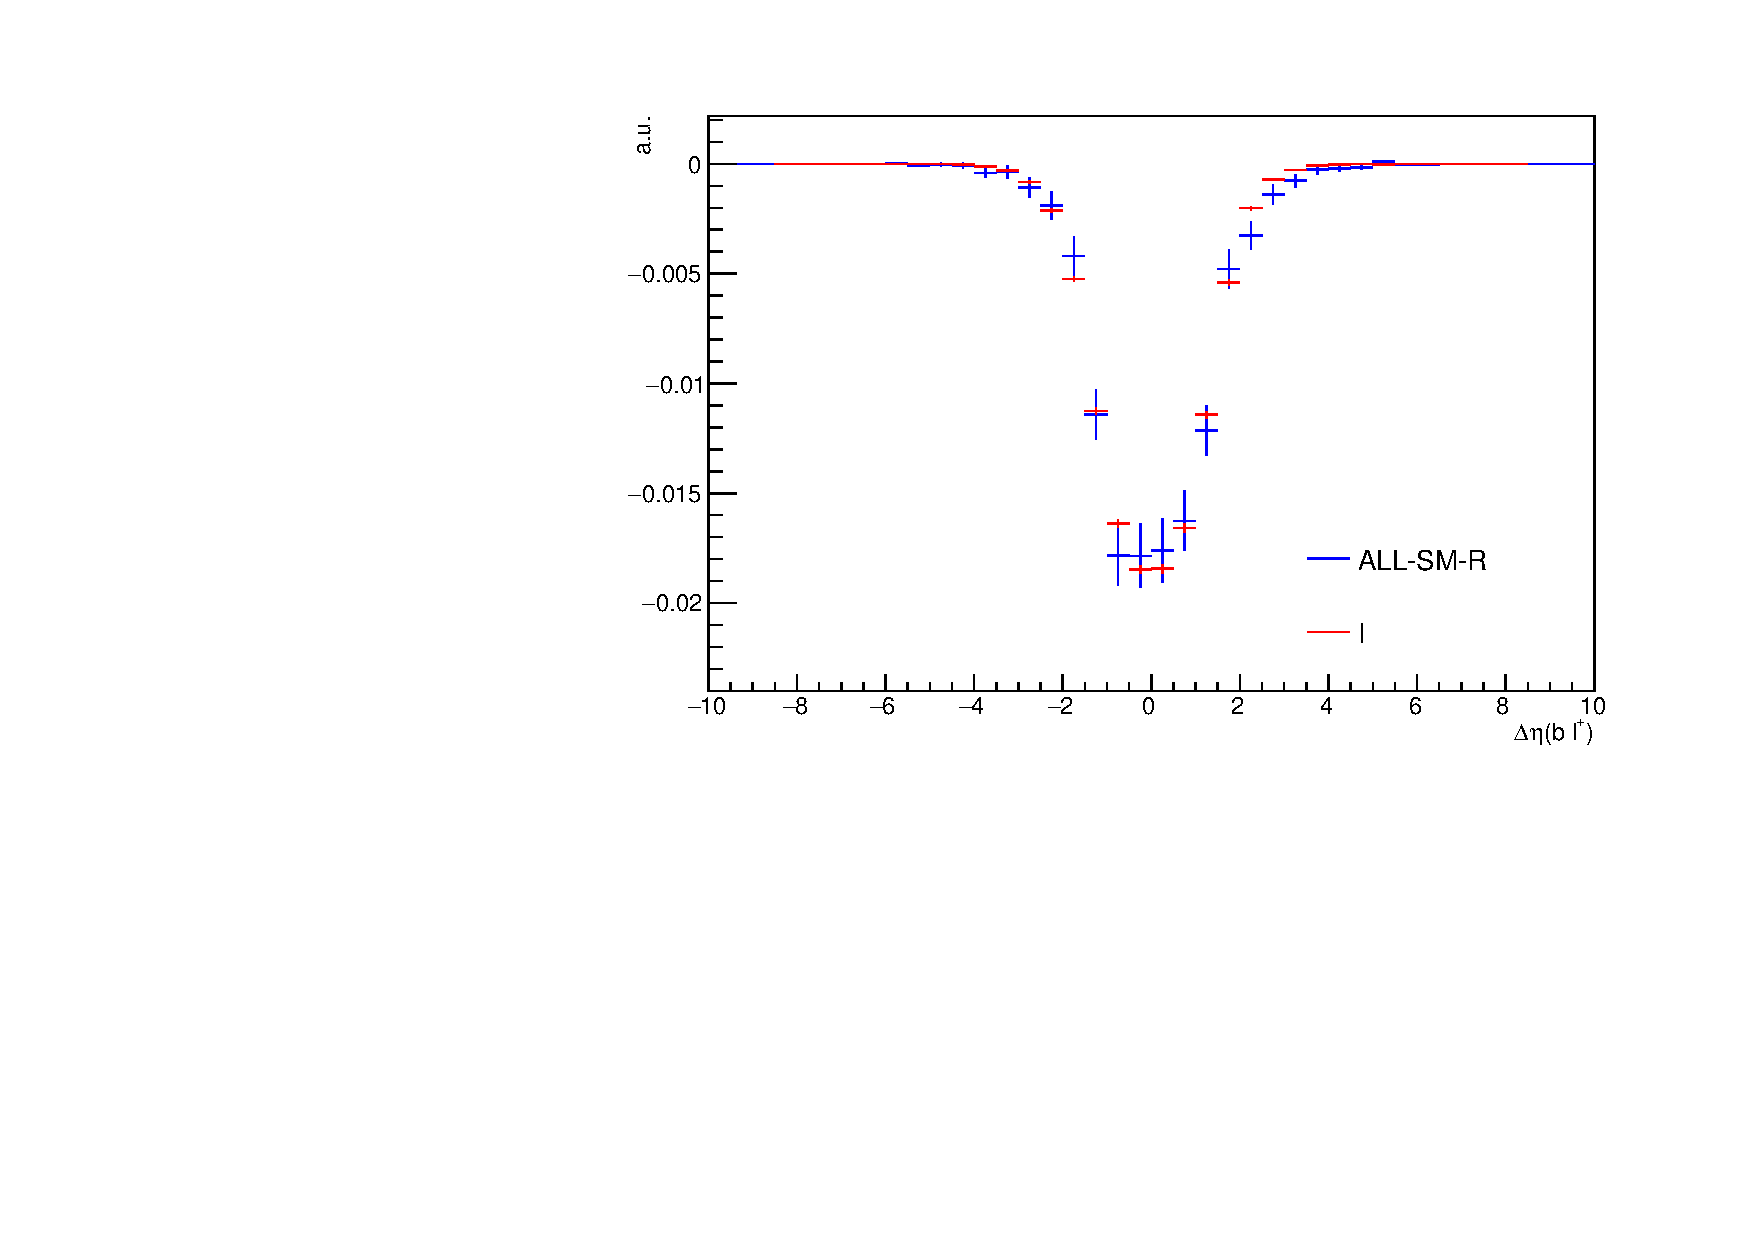
\includegraphics[width=0.4\textwidth]{fig/chapt4/gen_plots/blp_deltaEta_compare.pdf}
  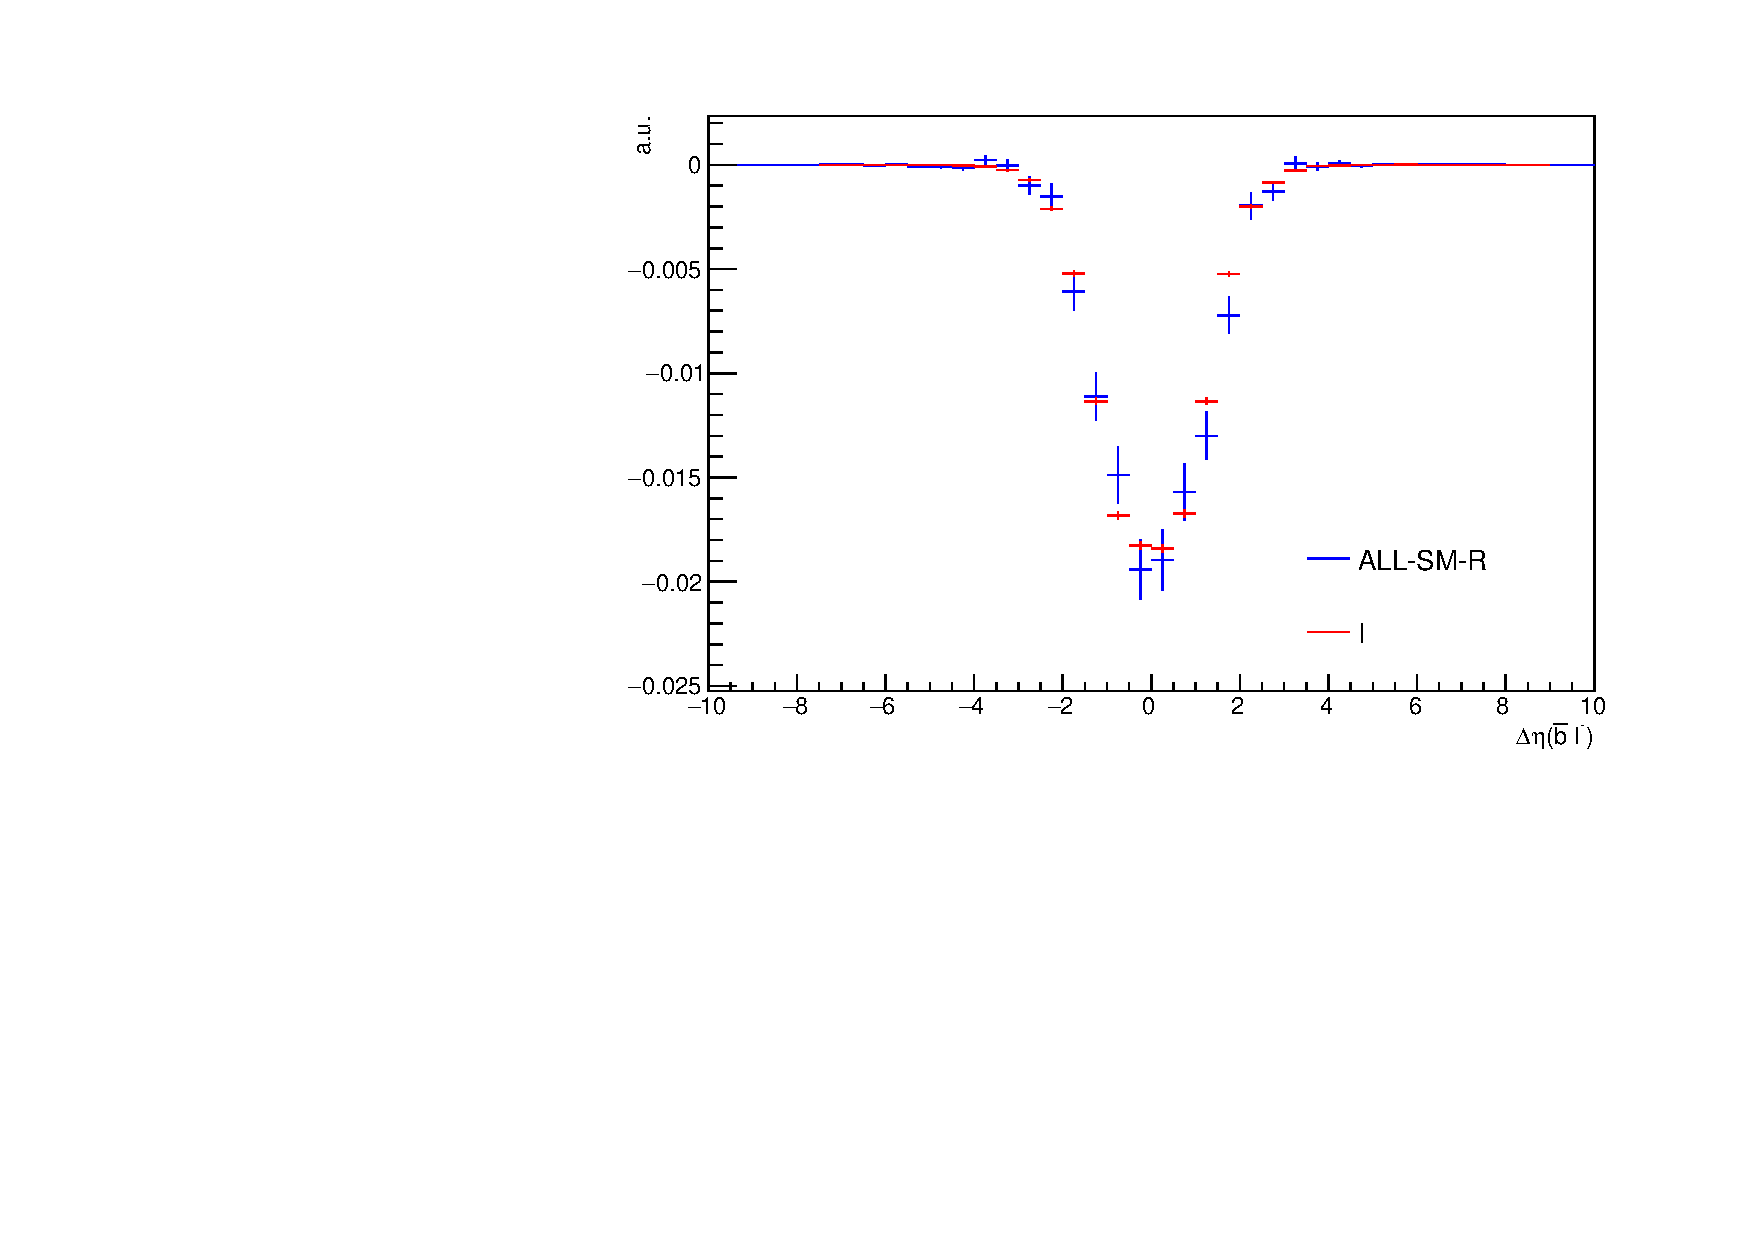
\includegraphics[width=0.4\textwidth]{fig/chapt4/gen_plots/bbarlm_deltaEta_compare.pdf}\\
  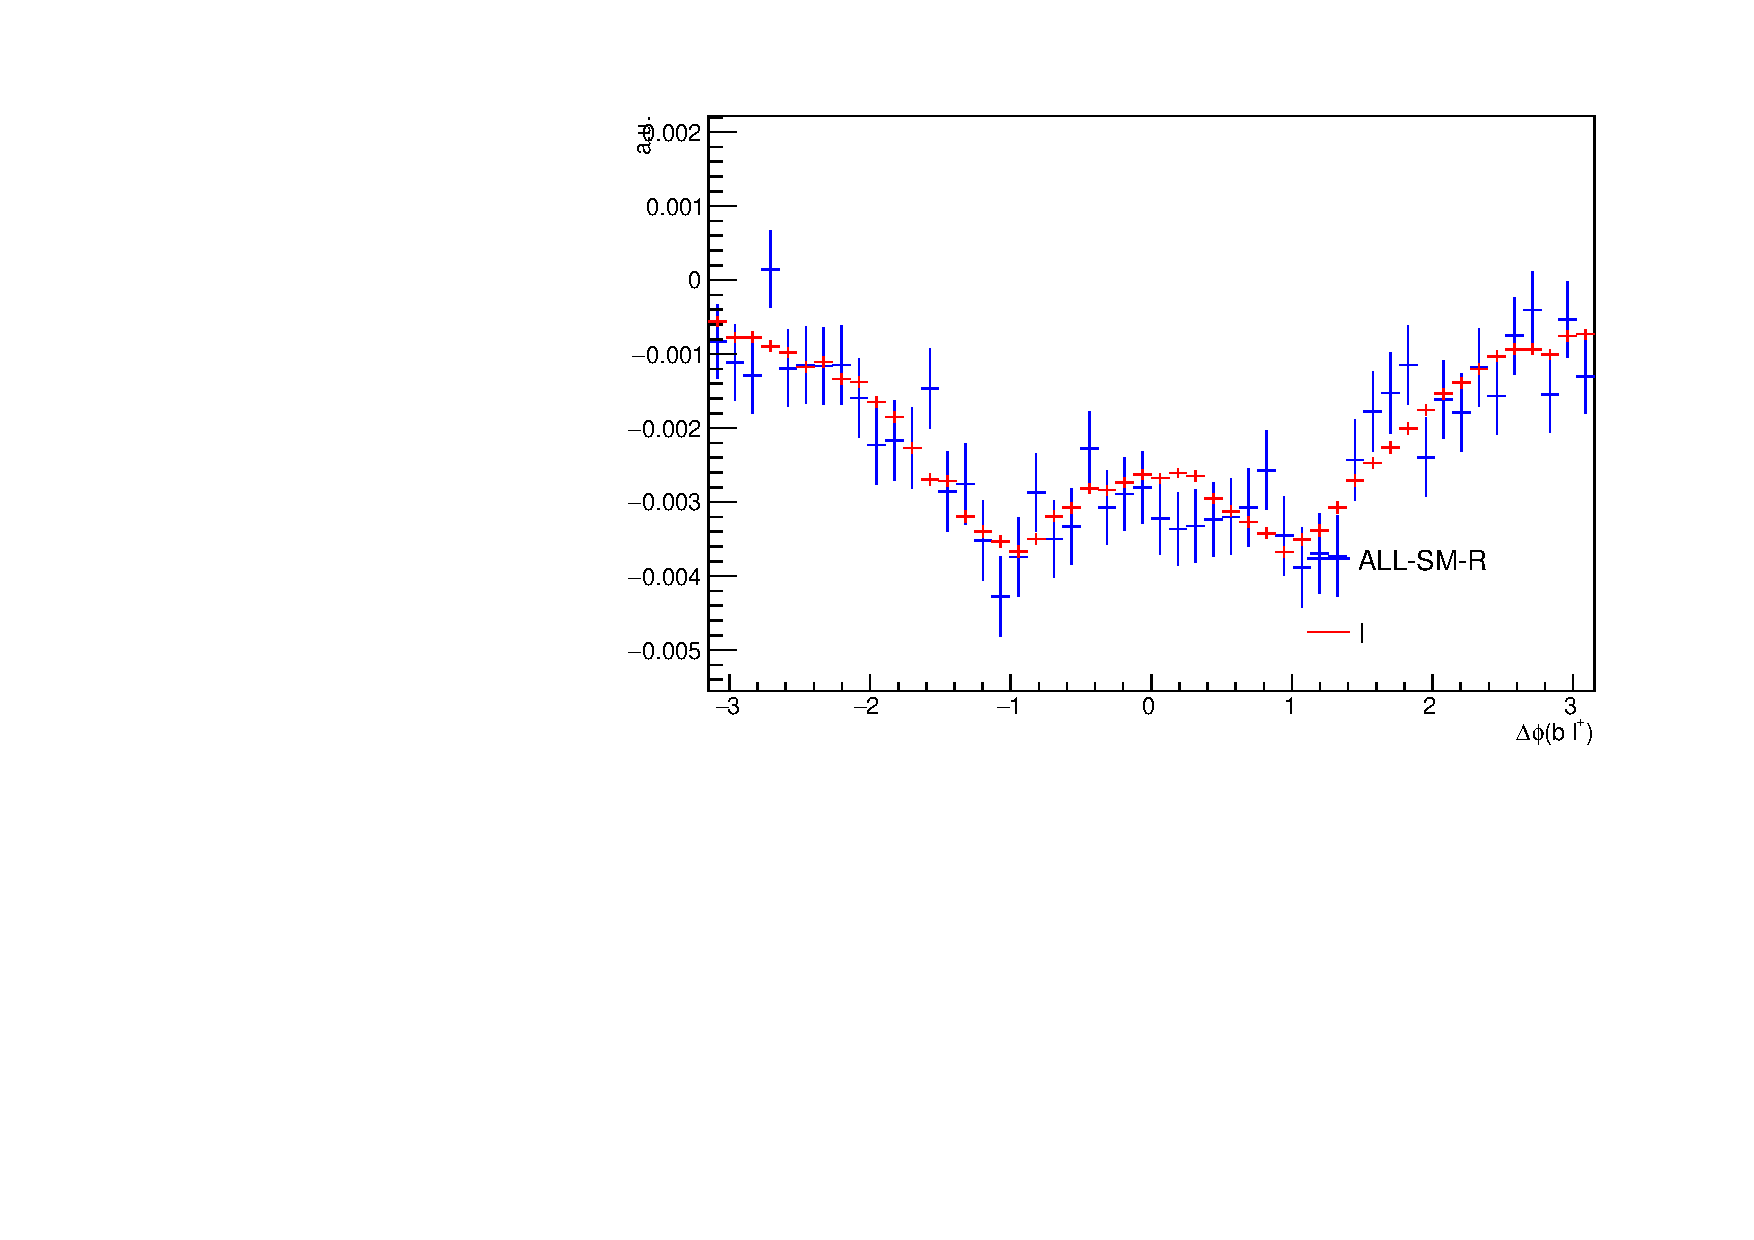
\includegraphics[width=0.4\textwidth]{fig/chapt4/gen_plots/blp_deltaphi_compare.pdf}
  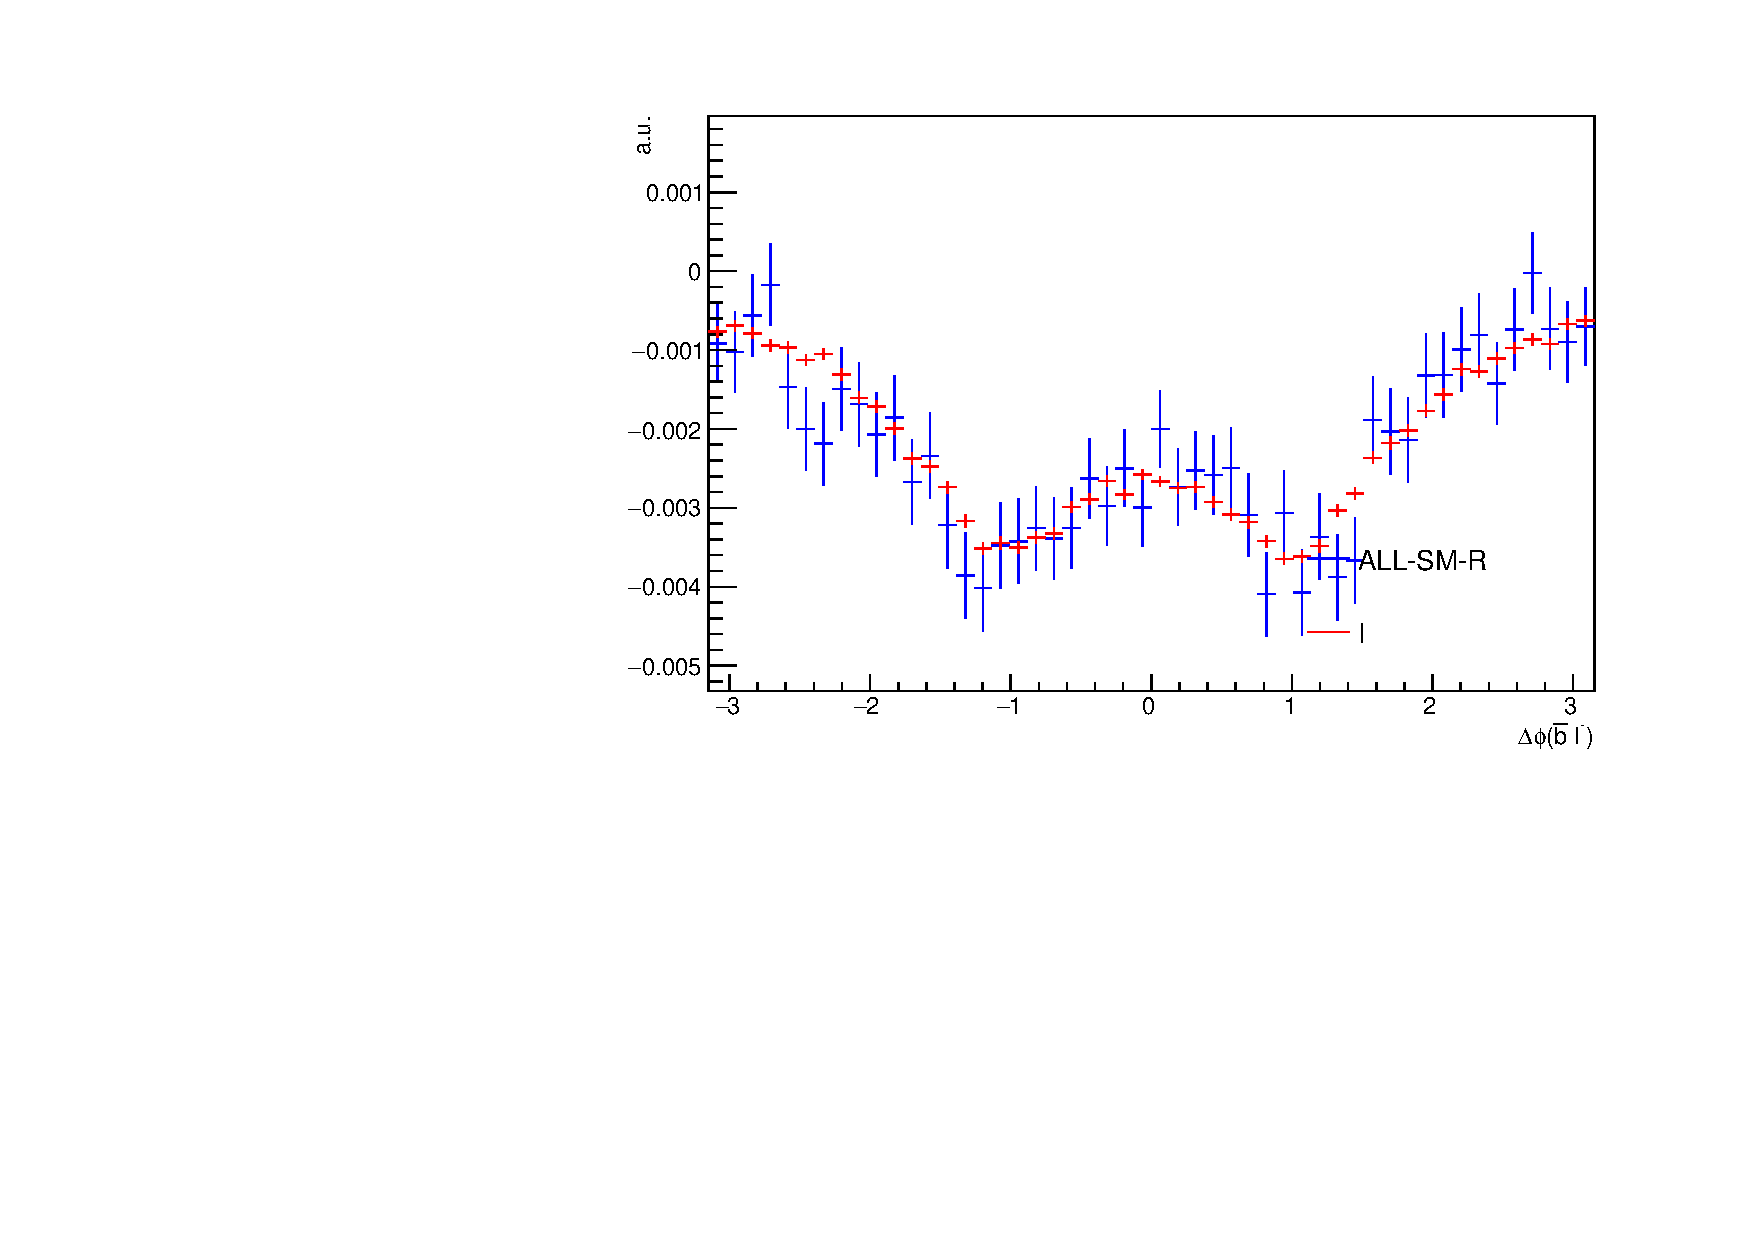
\includegraphics[width=0.4\textwidth]{fig/chapt4/gen_plots/bbarlm_deltaphi_compare.pdf}\\
  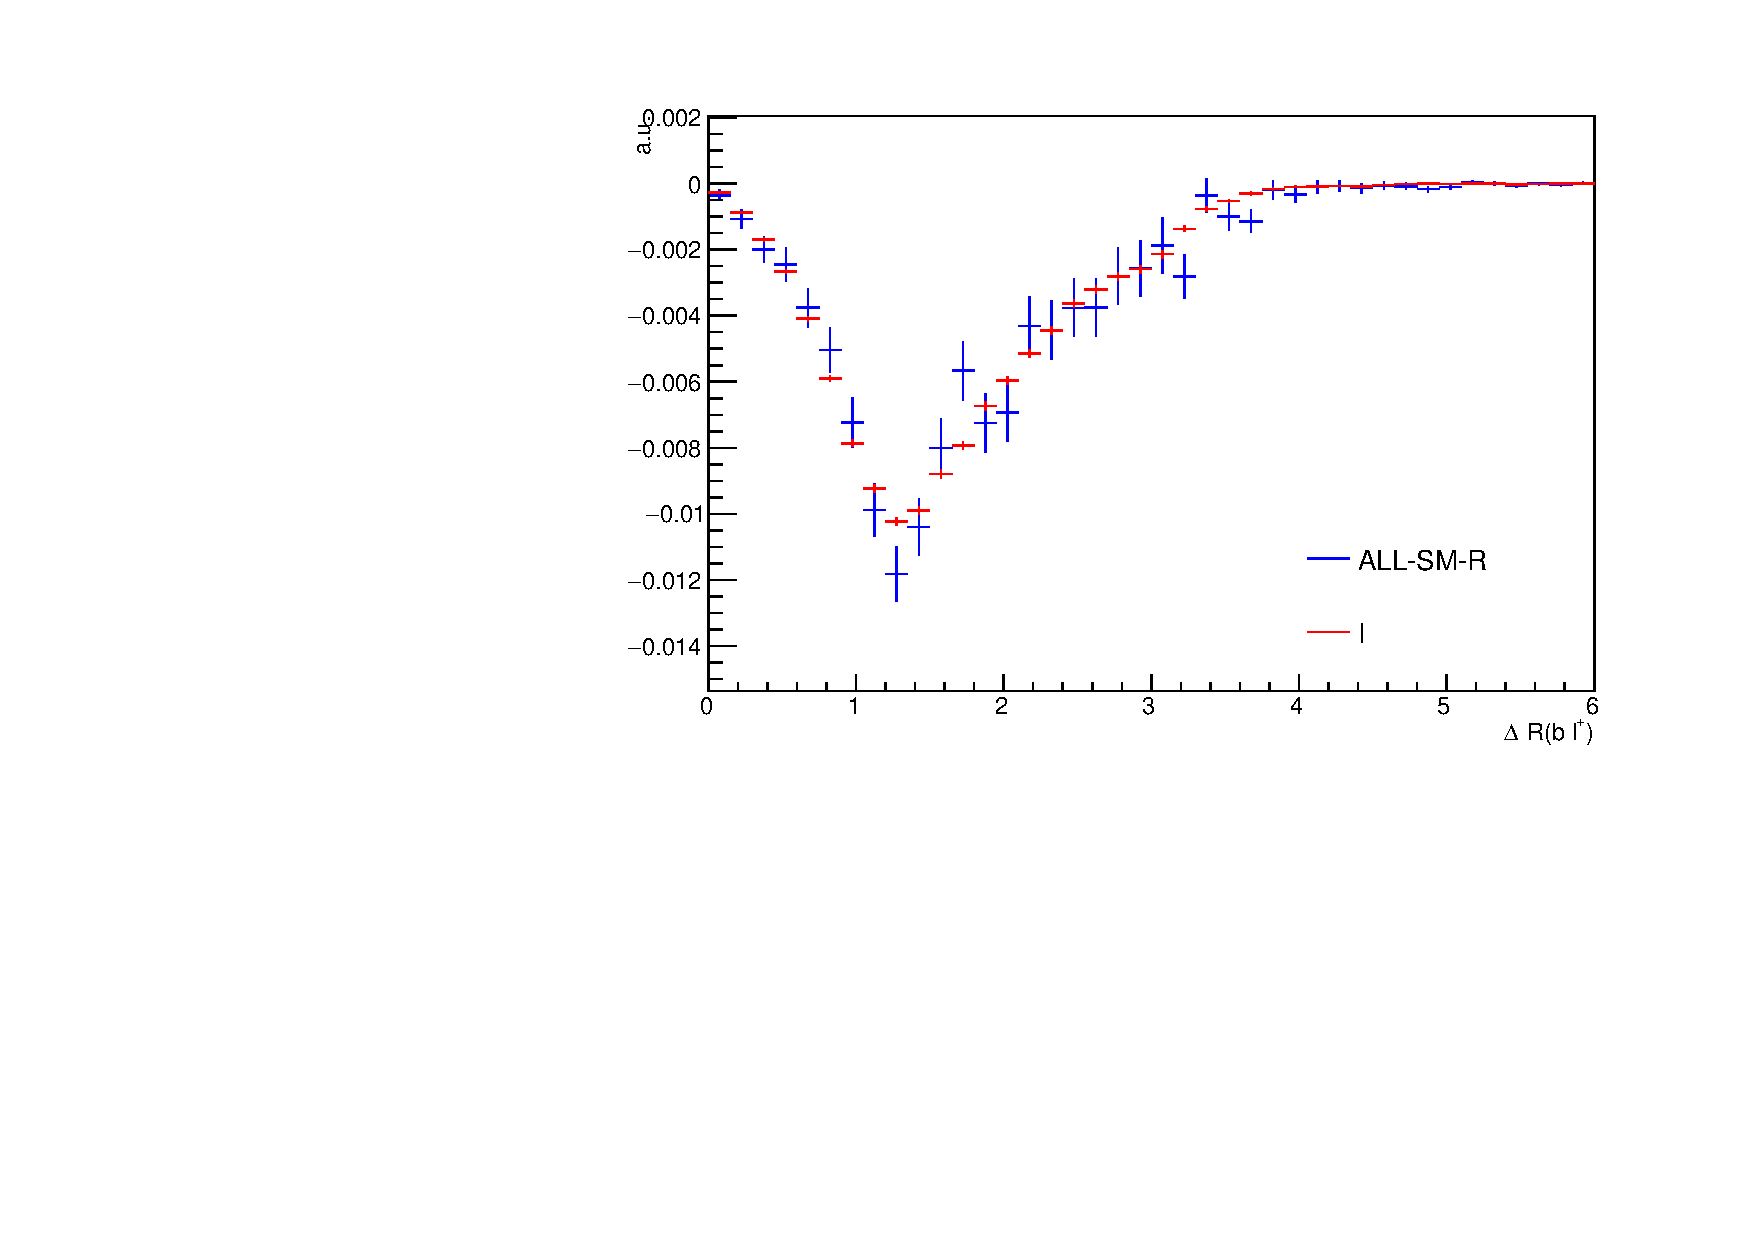
\includegraphics[width=0.4\textwidth]{fig/chapt4/gen_plots/blp_deltaR_compare.pdf}
  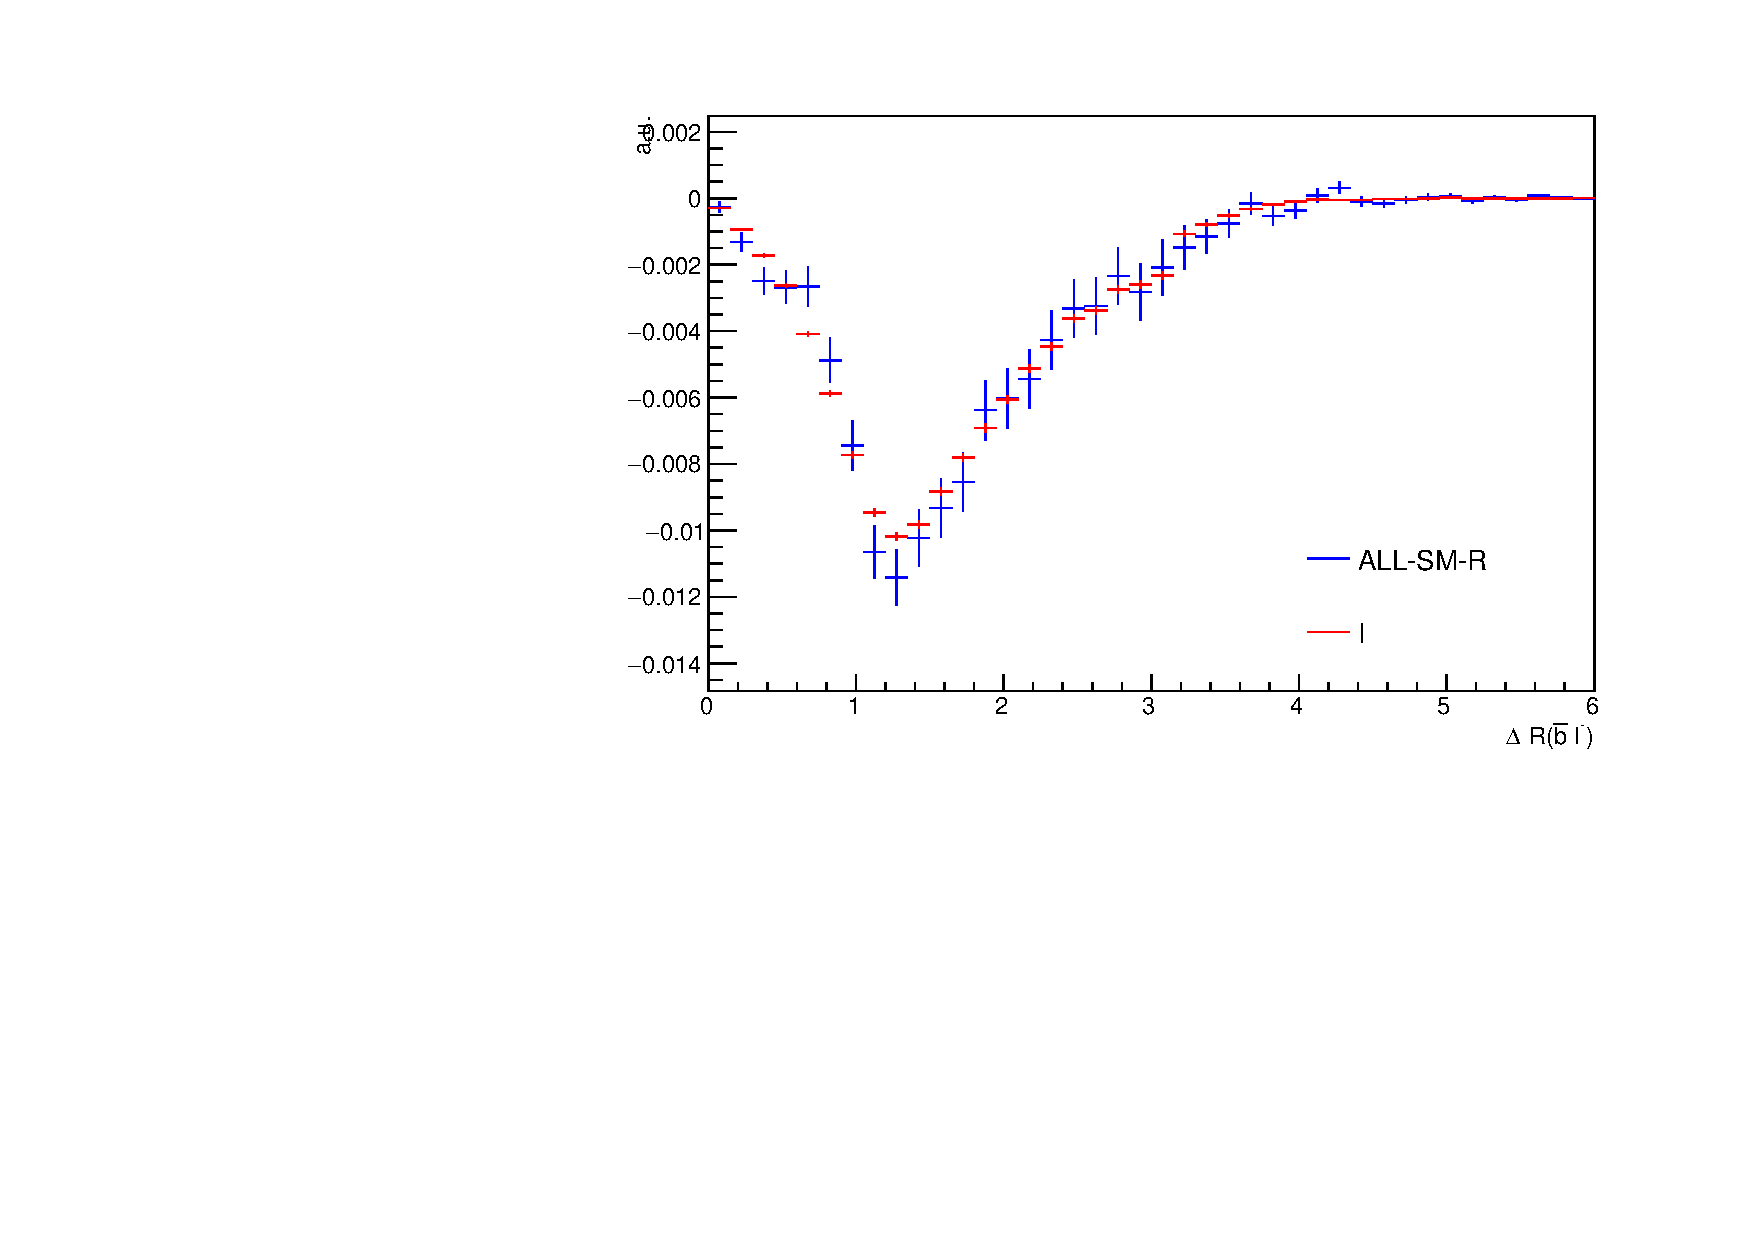
\includegraphics[width=0.4\textwidth]{fig/chapt4/gen_plots/bbarlm_deltaR_compare.pdf}
  \caption{Distributions of the $\Delta\eta$ (top), $\Delta\phi$ (middle) and $\Delta R$ (bottom) between the b~quark/antiquark and the charged lepton coming from the decay of the top quark (left) or the top antiquark (right). Comparison of the two approaches to model the interference.}
  \label{fig:comparison_b_relto_l}
\end{figure}

\begin{figure} \centering
  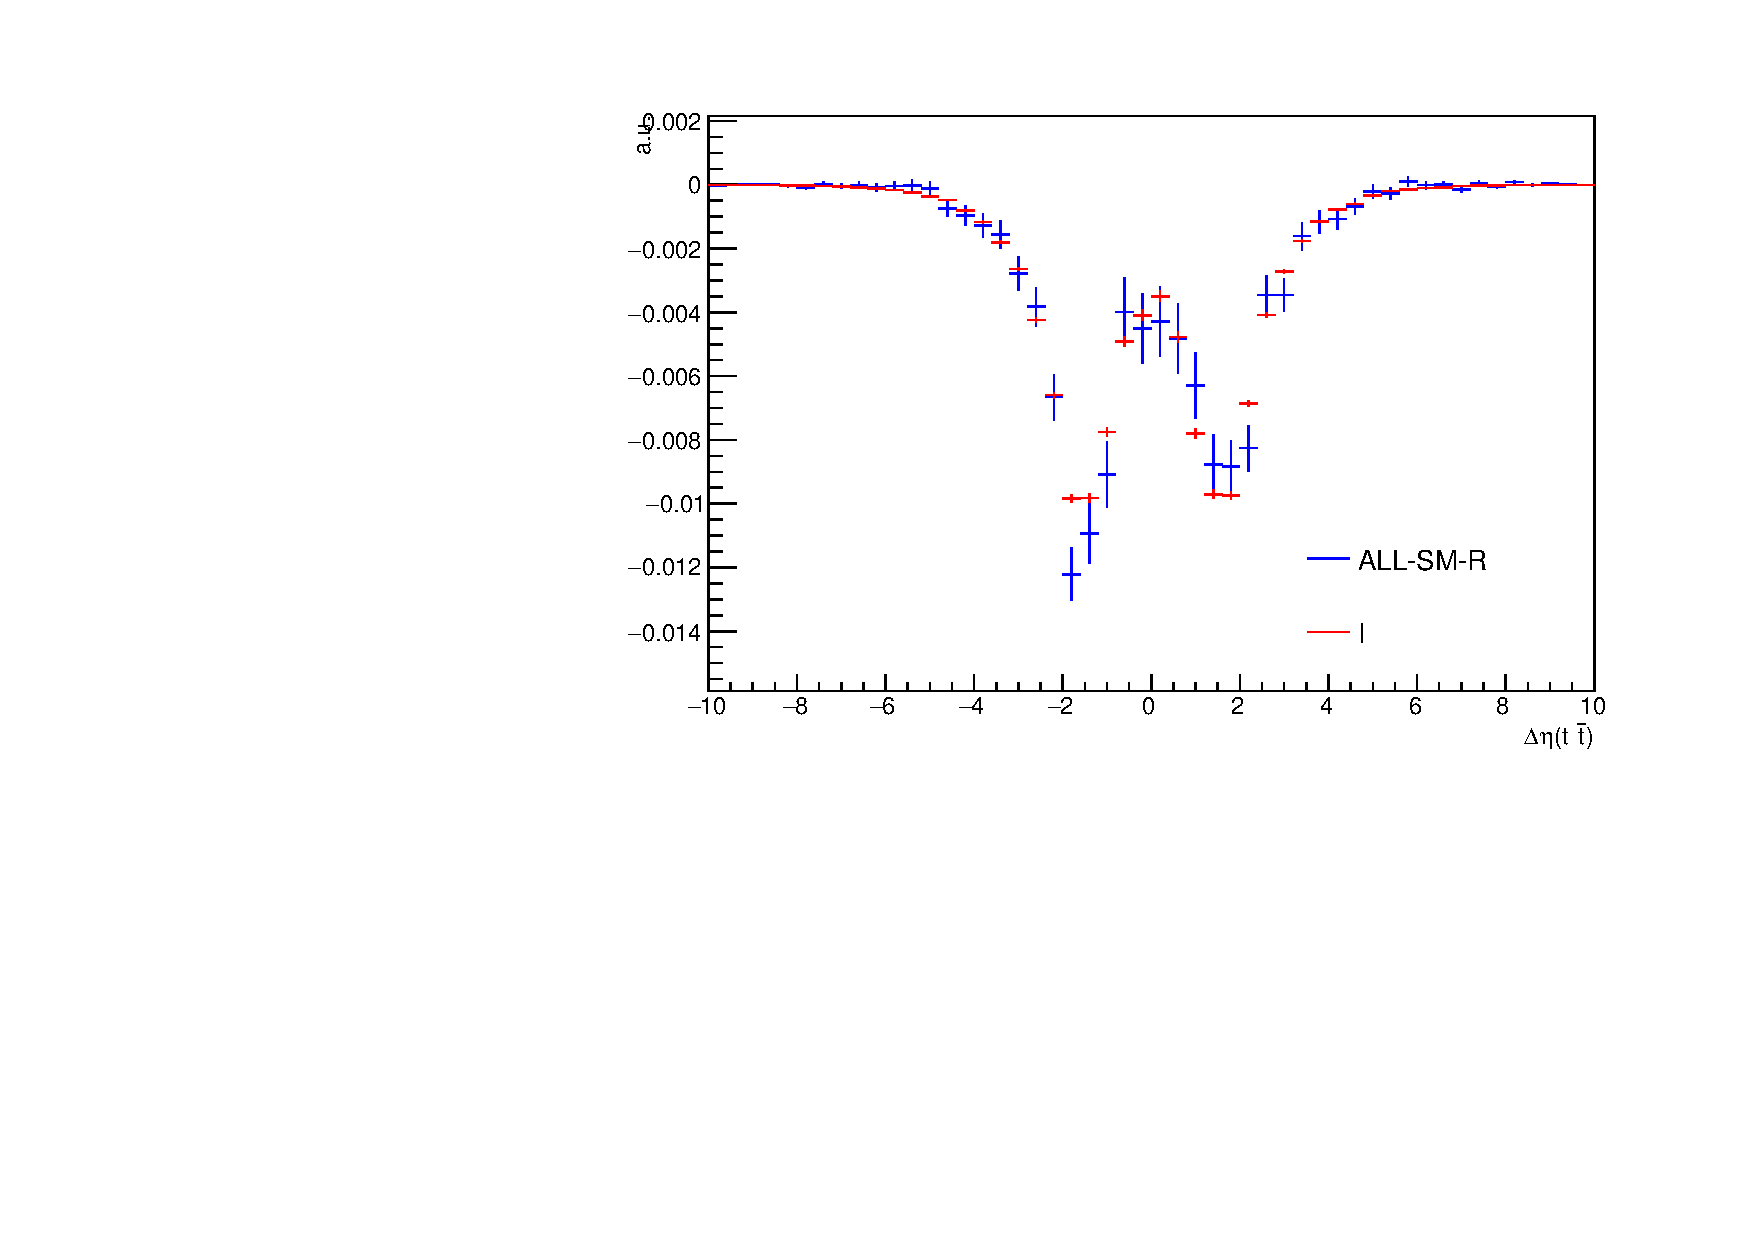
\includegraphics[width=0.4\textwidth]{fig/chapt4/gen_plots/ttbar_deltaEta_compare.pdf}
  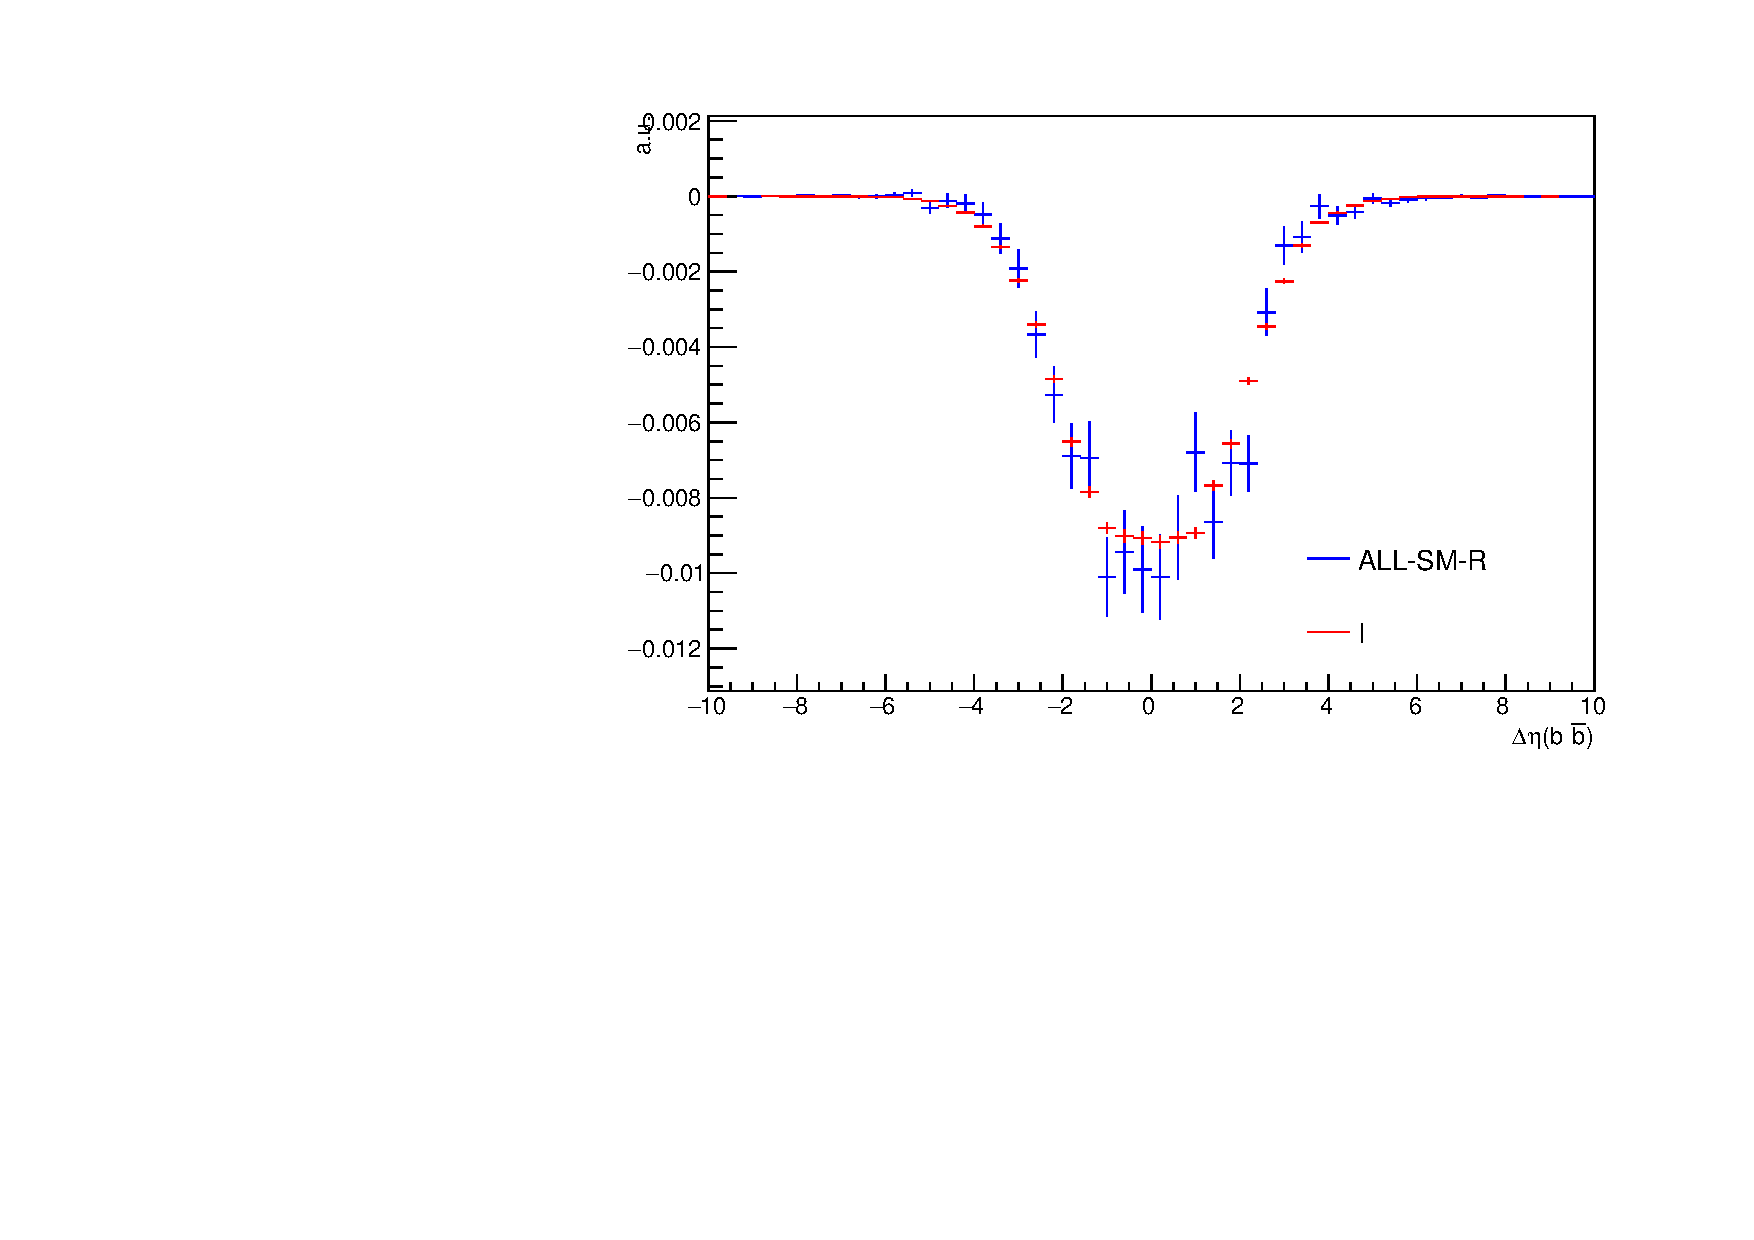
\includegraphics[width=0.4\textwidth]{fig/chapt4/gen_plots/bbbar_deltaEta_compare.pdf}\\
  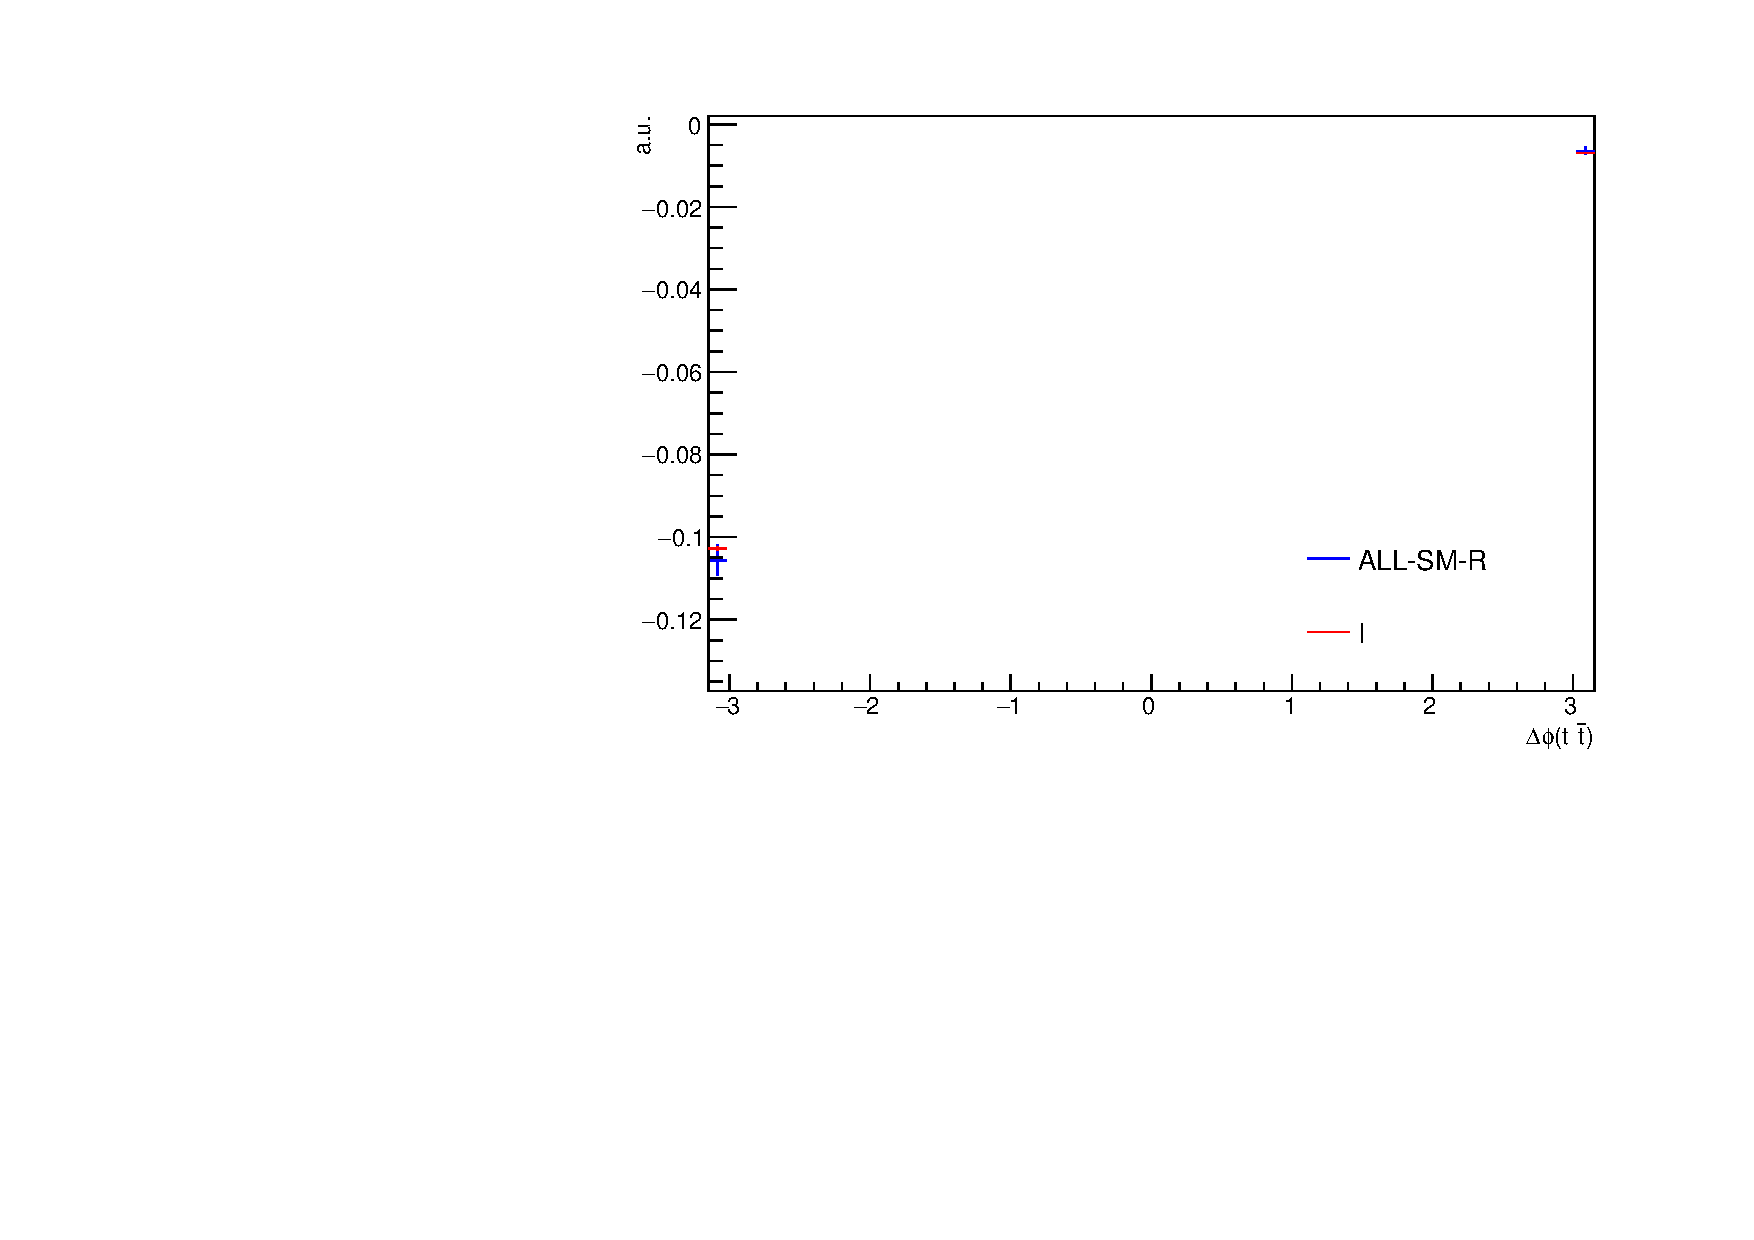
\includegraphics[width=0.4\textwidth]{fig/chapt4/gen_plots/ttbar_deltaphi_compare.pdf}
  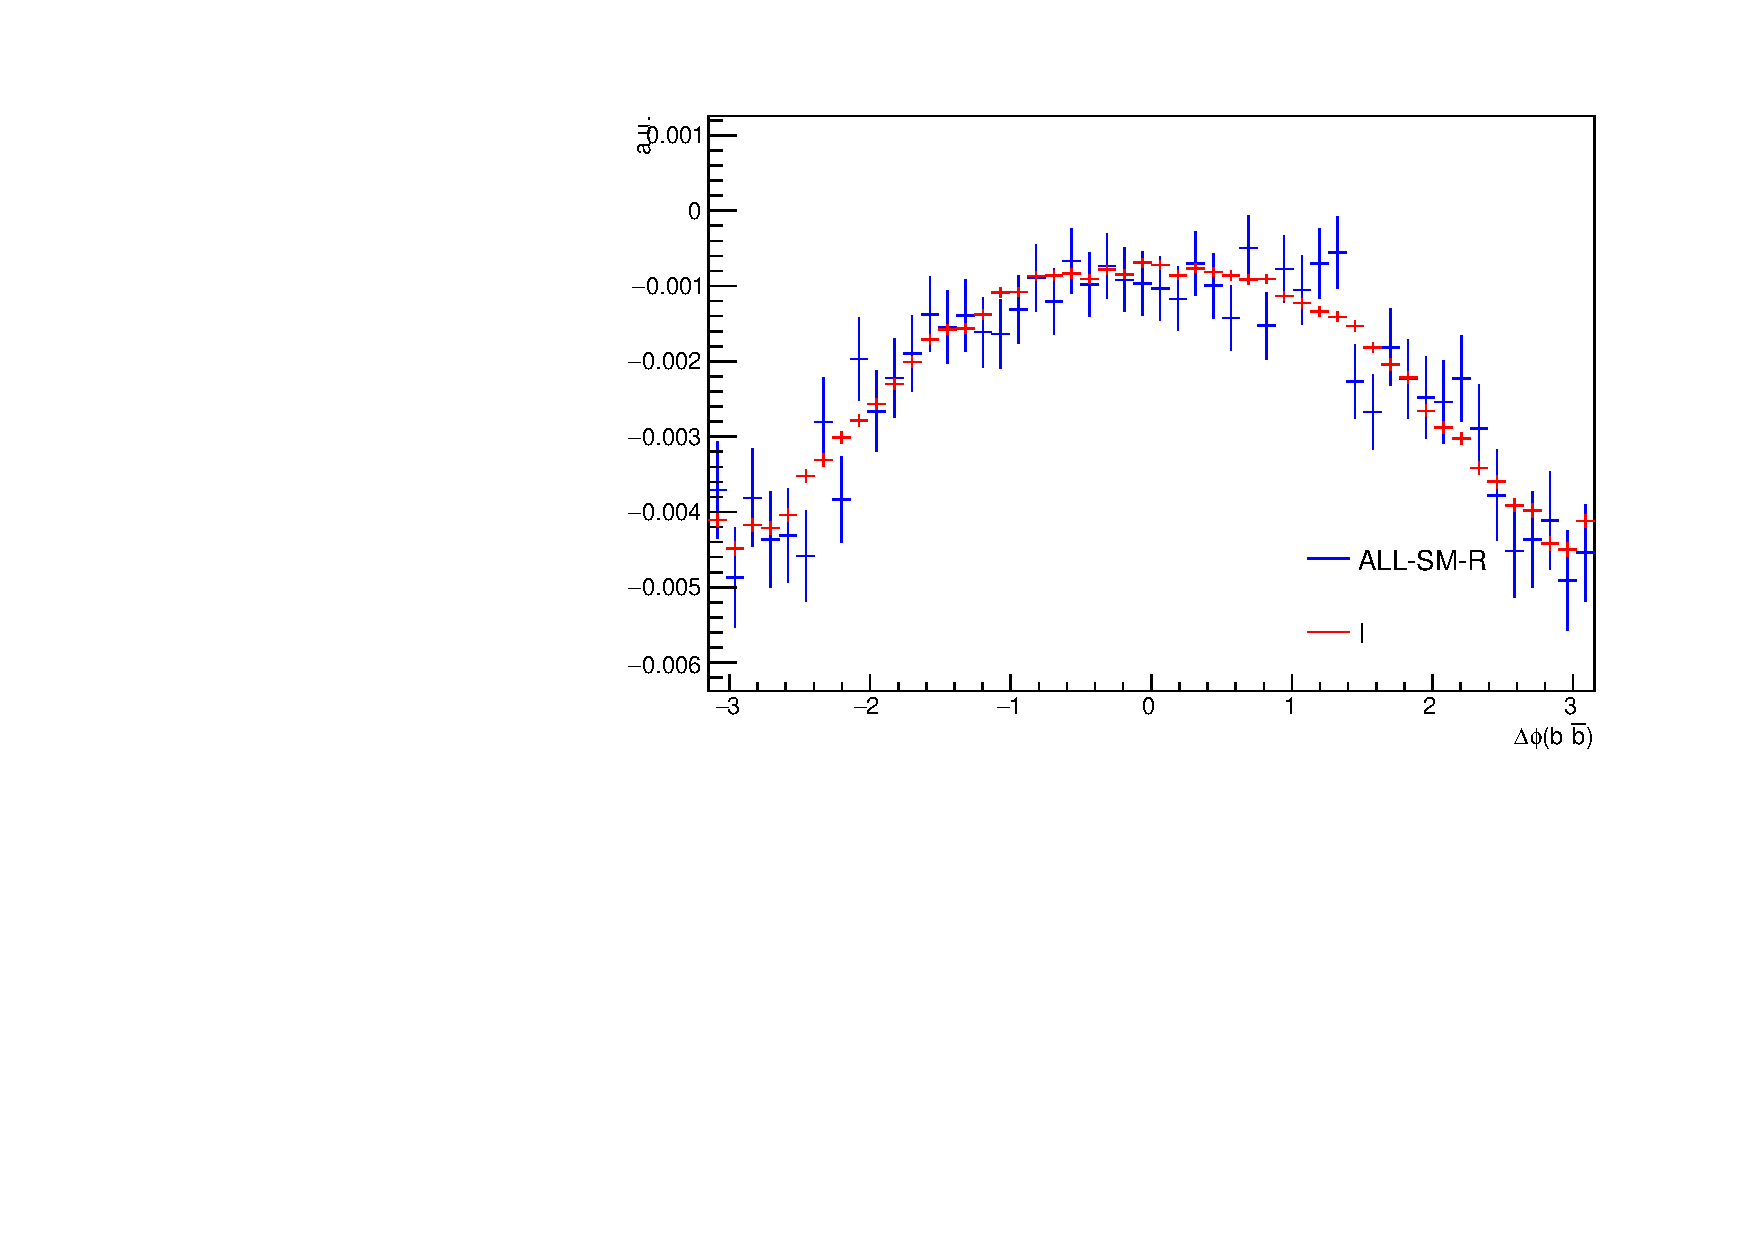
\includegraphics[width=0.4\textwidth]{fig/chapt4/gen_plots/bbbar_deltaphi_compare.pdf}\\
  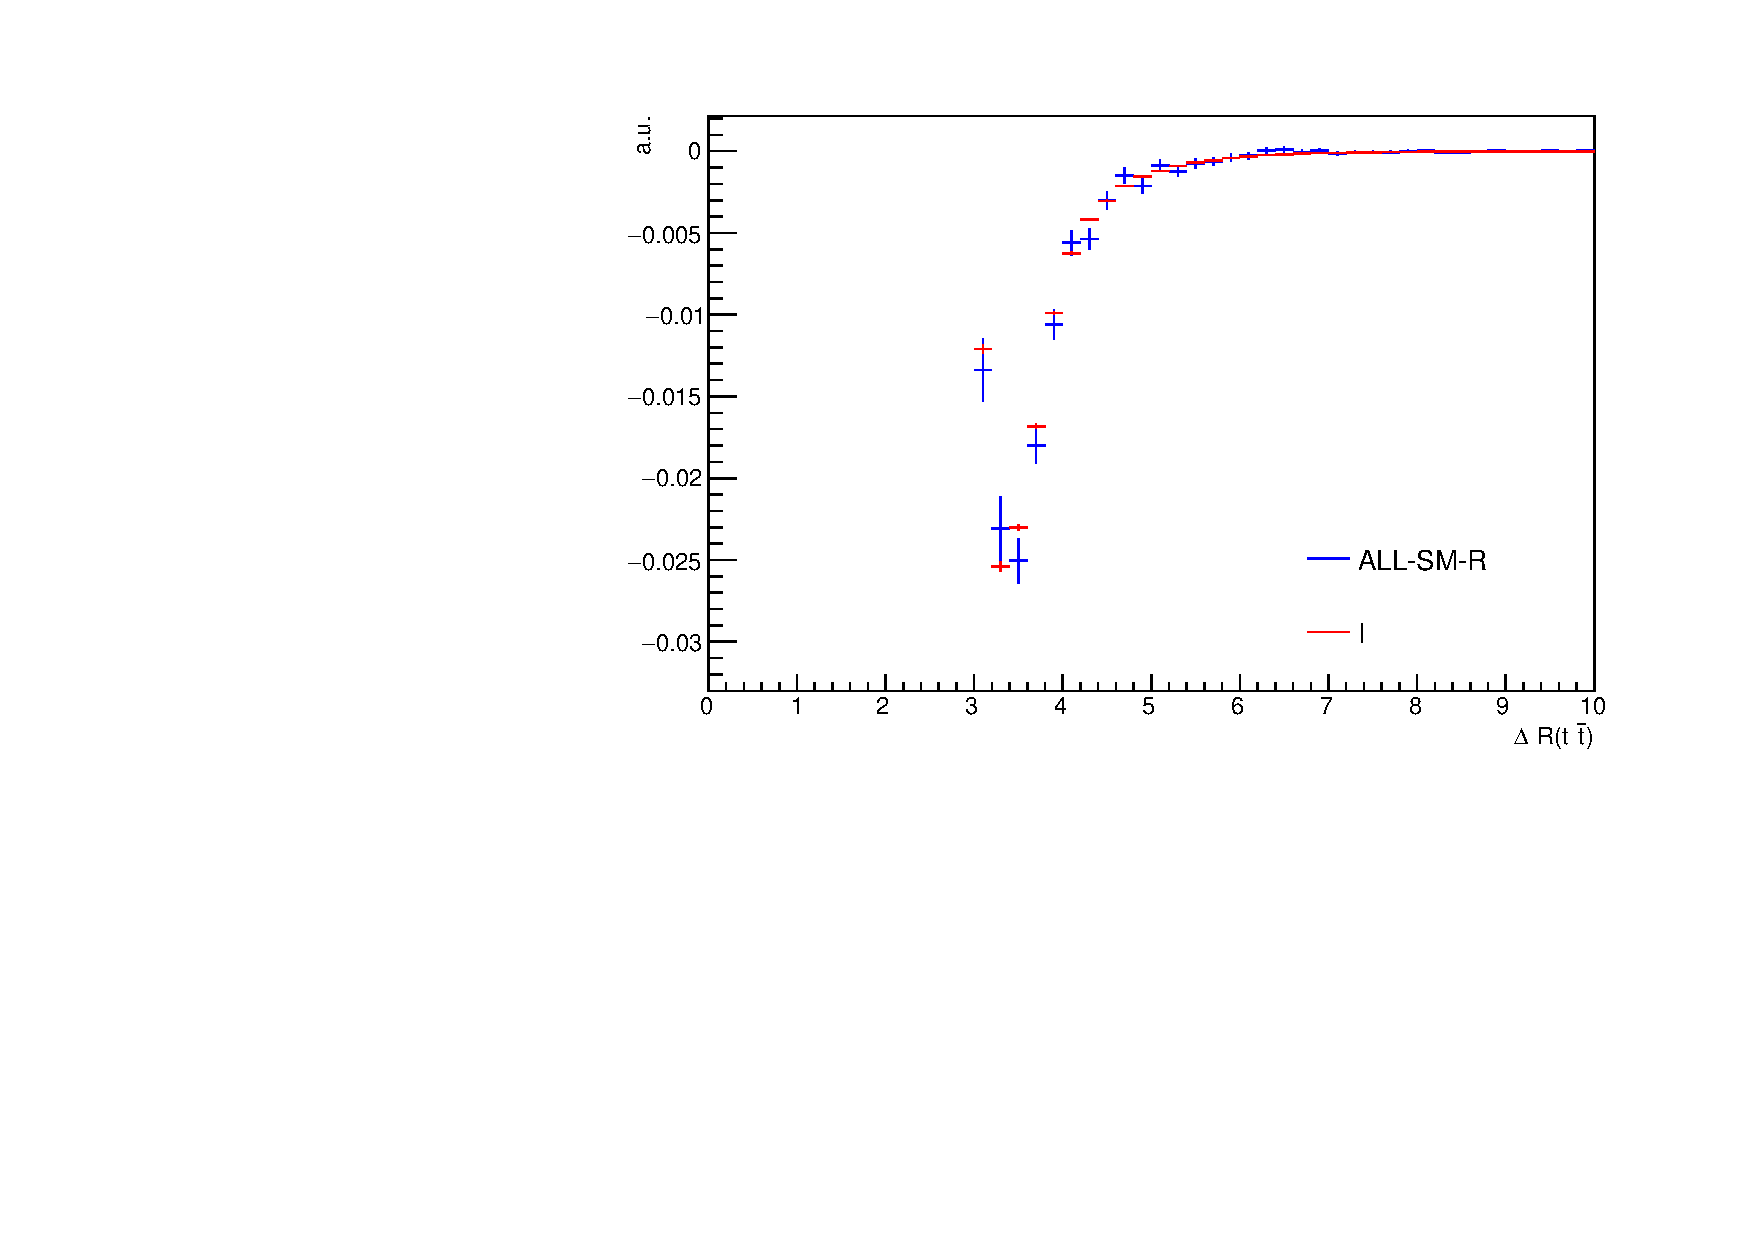
\includegraphics[width=0.4\textwidth]{fig/chapt4/gen_plots/ttbar_deltaR_compare.pdf}
  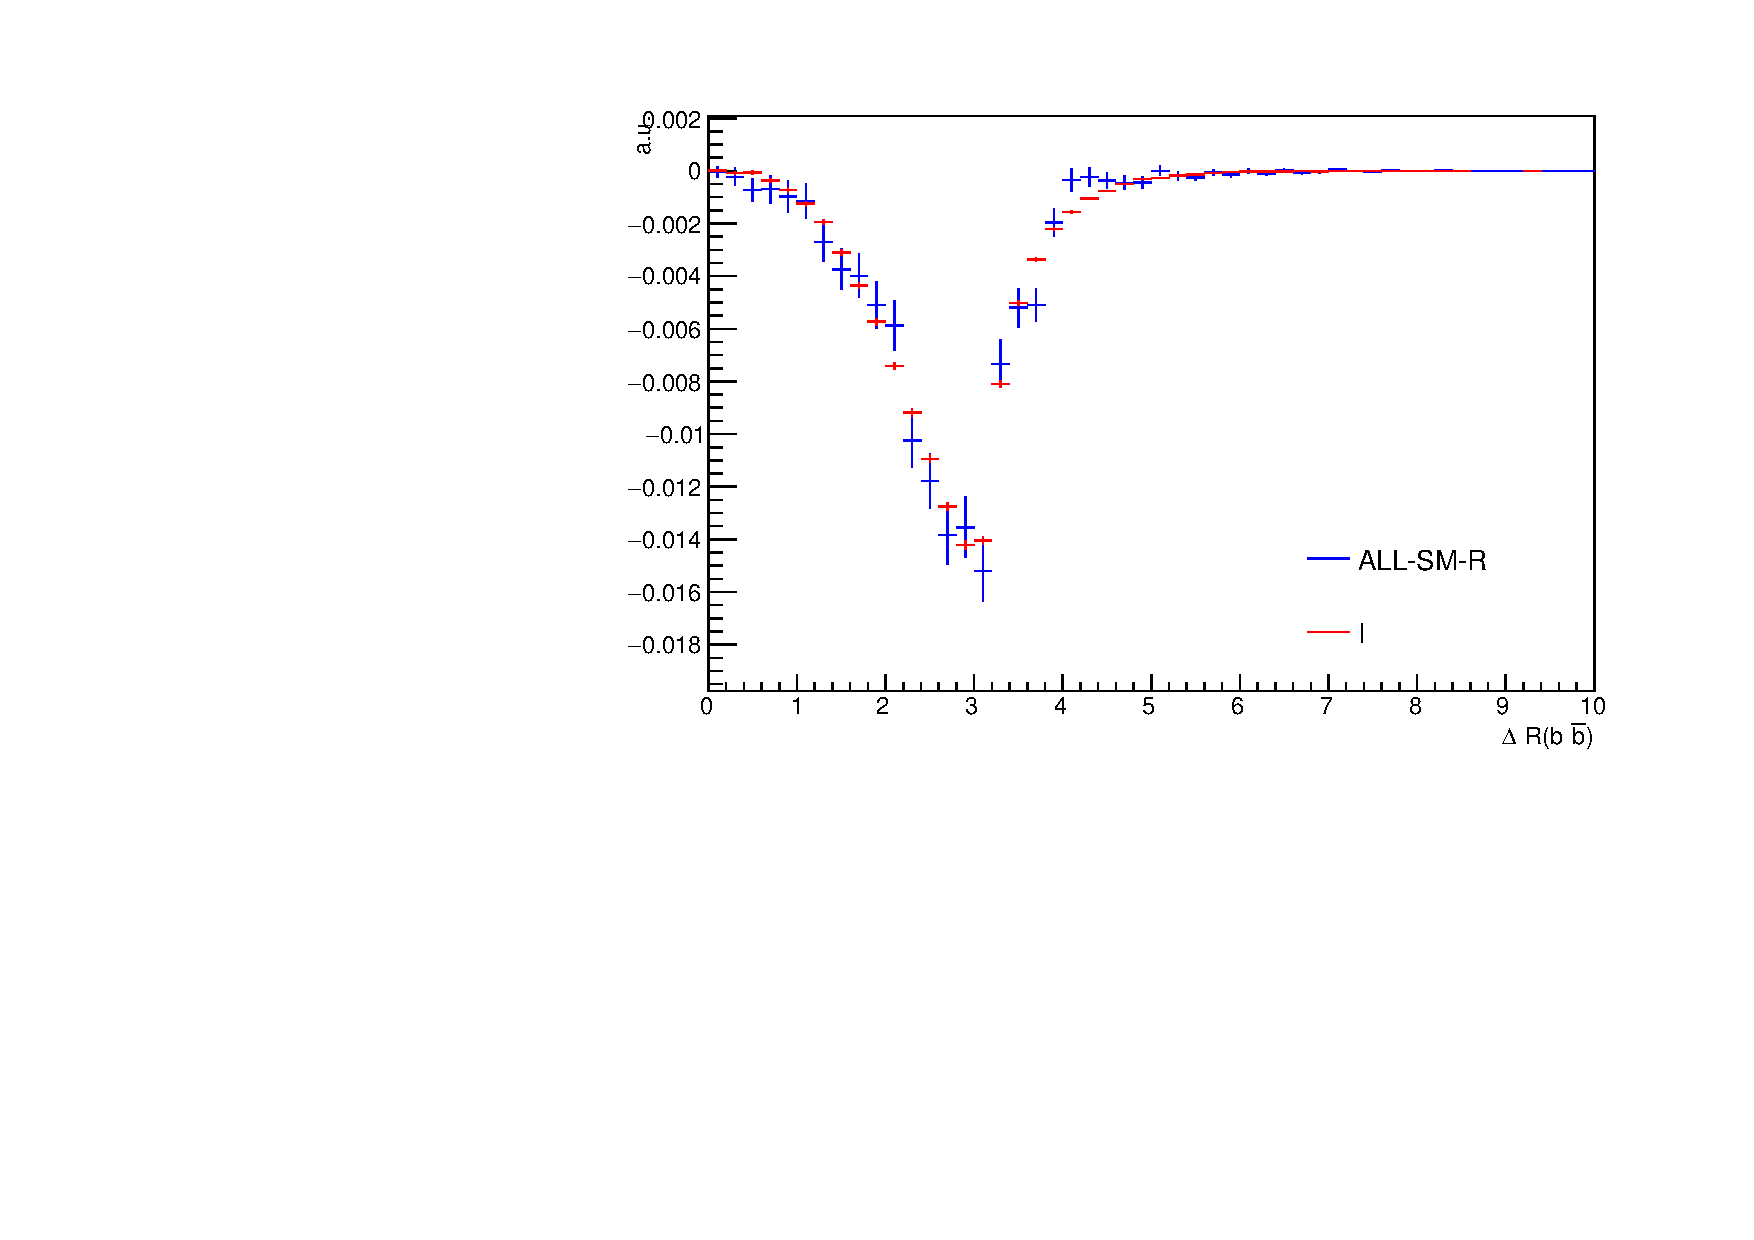
\includegraphics[width=0.4\textwidth]{fig/chapt4/gen_plots/bbbar_deltaR_compare.pdf}
  \caption{Distributions of the $\Delta\eta$ (top), $\Delta\phi$ (middle) and $\Delta R$ (bottom) between the top quark and antiquark (left) and the b~quark and antiquark (right) coming from decays of the top quarks. Comparison of the two approaches to model the interference.}
  \label{fig:comparison_ttbar_bbbar}
\end{figure}

\begin{figure} \centering
  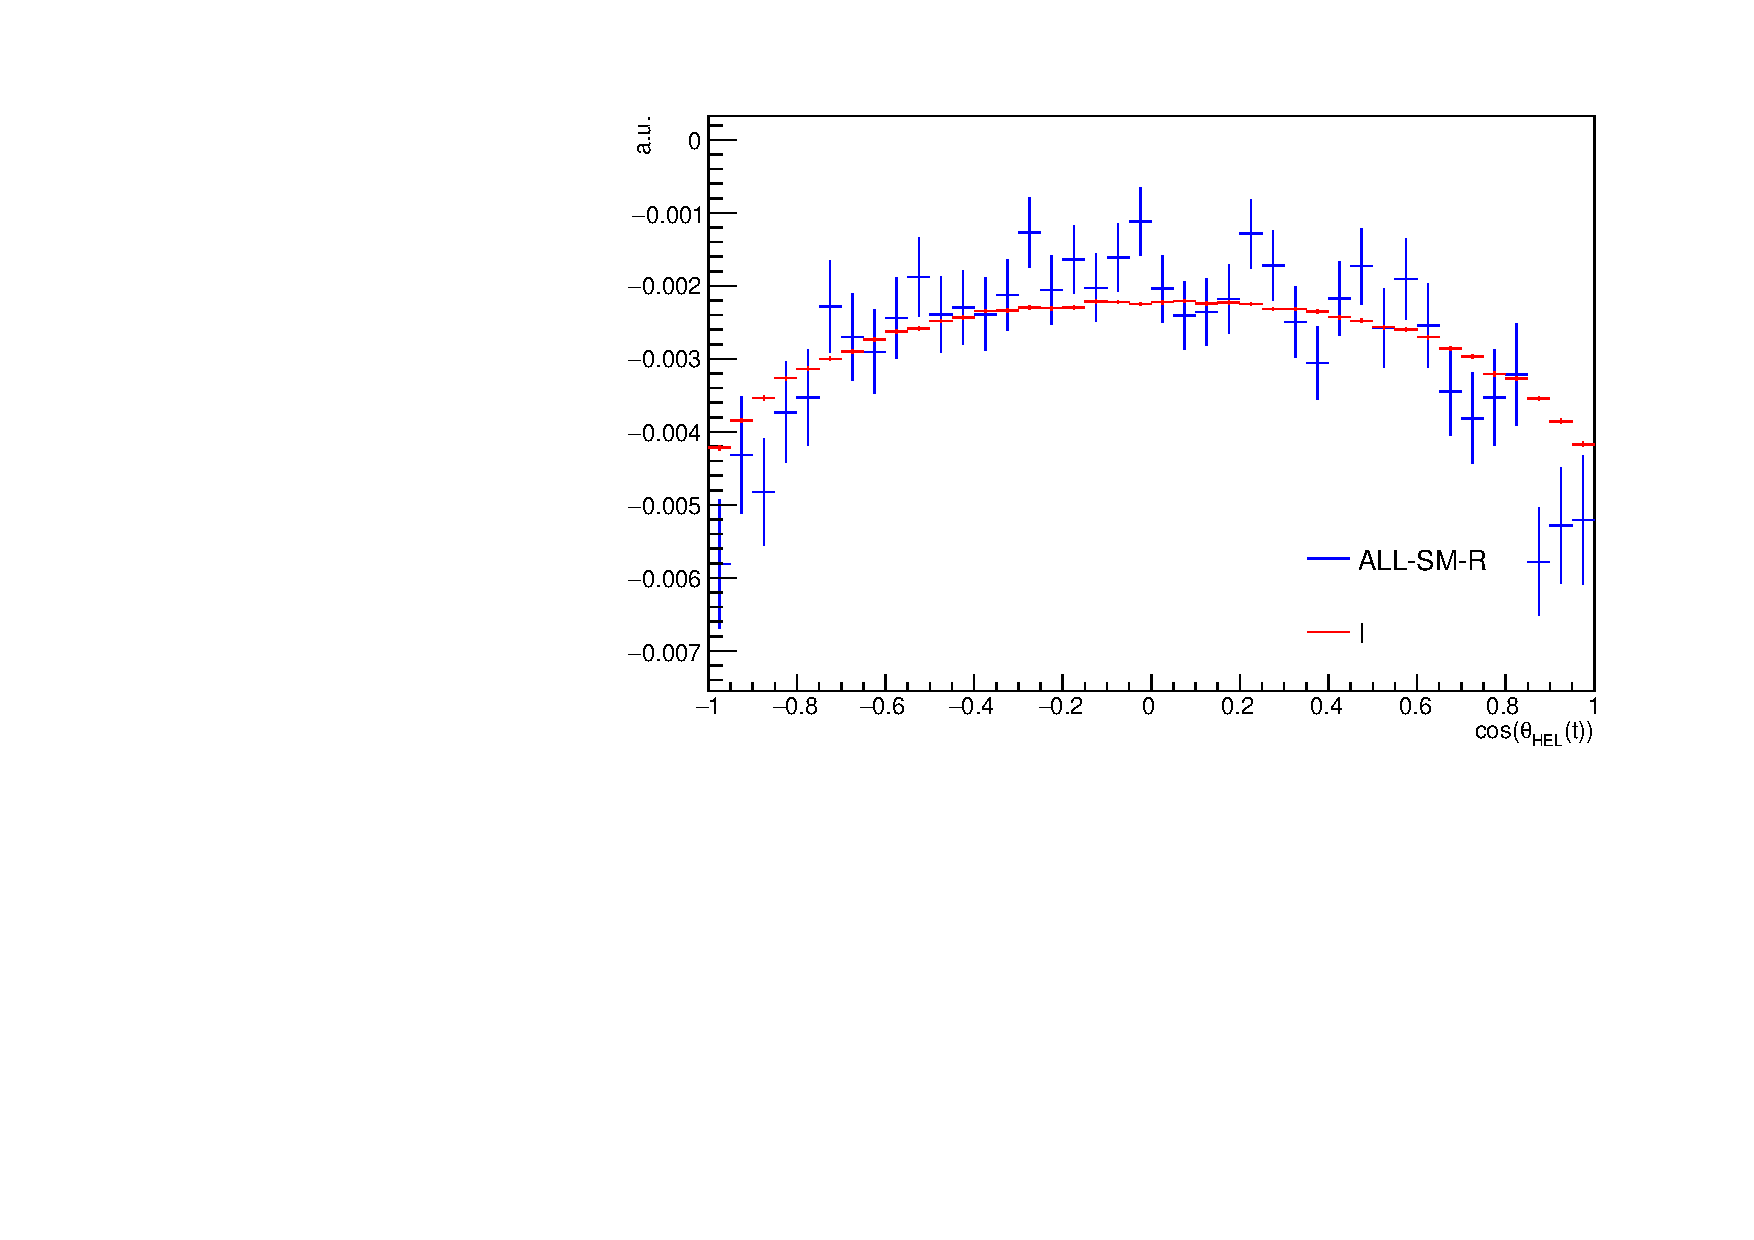
\includegraphics[width=0.4\textwidth]{fig/chapt4/gen_plots/top_theta_hel_compare.pdf}
  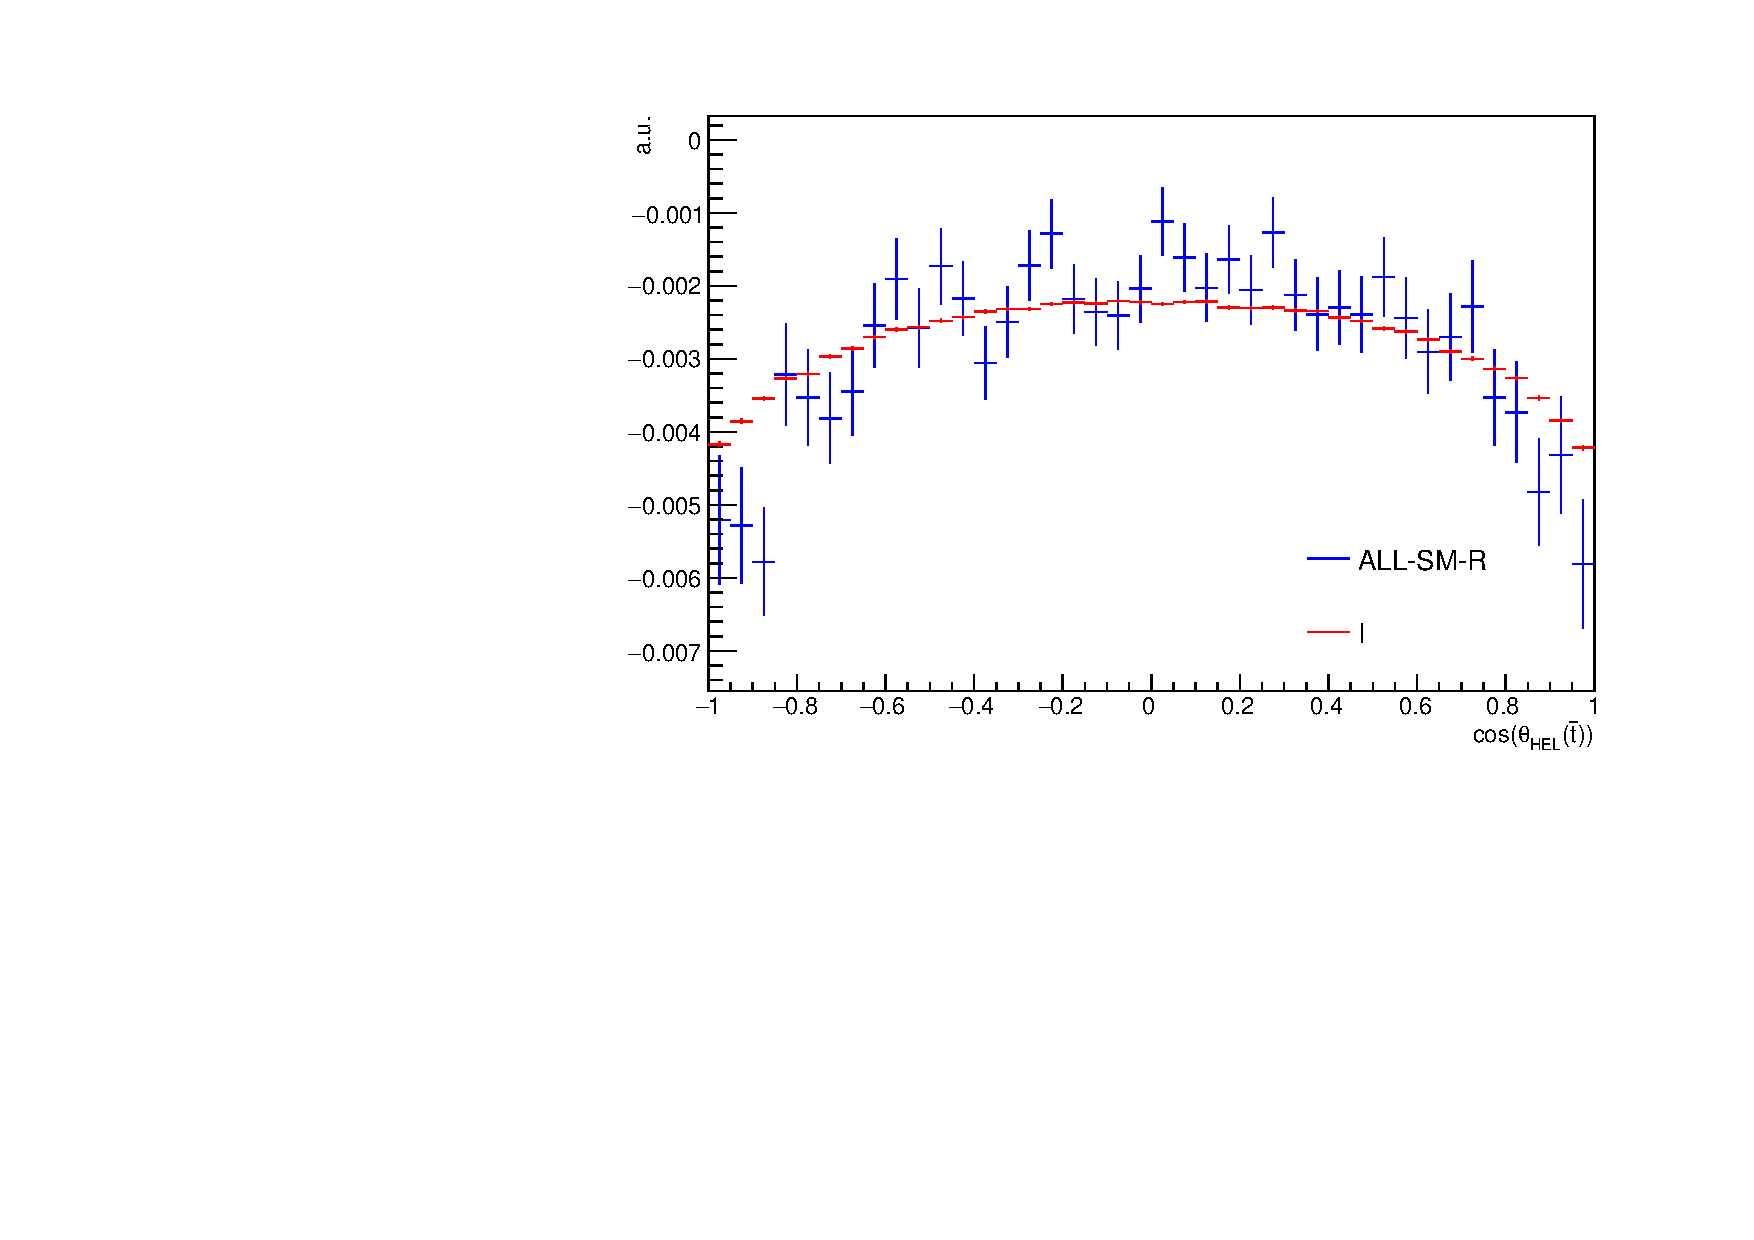
\includegraphics[width=0.4\textwidth]{fig/chapt4/gen_plots/tbar_theta_hel_compare.pdf}
  \caption{Distributions of the cosine of the angle between the three-momentum of the top quark (left) and antiquark (right) in the center-of-mass frame of the $t\bar t$~system, and the three-momentum of the $t\bar t$~system in the laboratory frame. Comparison of the two approaches to model the interference.}
  \label{fig:comparison_tophel}
\end{figure}


\clearpage{\pagestyle{empty}\cleardoublepage}
